\clearpage{\pagestyle{empty}\cleardoublepage}

\chapter{\wbx\ analysis: data to background comparison in SDRs}\label{app:wbxSDRs}

\section{Comparison between data and prediction in SDR0}
\label{sec:DataMC_CR0}

SDR0: preselection cuts, $\geq 1$ $W_{\rm had}$ candidates, $\HT<800\gev$. 

%%%%%%%%%%%%%%%
\begin{table}[h!]
\begin{center}
\renewcommand{\arraystretch}{1.3}
\begin{tabular}{l*{1}{r@{ $\pm$ }r@{ }l}}
\hline\hline
 & \multicolumn{3}{c}{ELEMUONCR0\_1W}\\
\hline
$T\bar{T}(600\GeV)$ (Chiral) & $7.05$ & $0.87$ & $^{+1.01}_{-1.76}$\\
\hline
$t\bar{t}$ & $4760.66$ & $43.08$ & $^{+805.03}_{-837.88}$\\
$W$+jets & $409.22$ & $29.61$ & $^{+169.34}_{-136.66}$\\
$Z$+jets & $86.14$ & $11.27$ & $^{+42.07}_{-45.56}$\\
Diboson & $7.95$ & $0.95$ & $^{+2.04}_{-2.28}$\\
Single top & $305.21$ & $11.66$ & $^{+43.96}_{-35.20}$\\
$t\bar{t}$$V$ & $44.46$ & $0.53$ & $^{+13.57}_{-13.66}$\\
Multijet & $27.22$ & $7.44$ & $ \pm\ 13.61$\\
\hline
Total bkg. & $5640.87 $ & $ 55.24$ & $ ^{+946.22}_{-948.39}$\\
\hline
Data & \multicolumn{3}{c}{$6042$}\\
\hline\hline
\end{tabular}

\vspace{0.5cm}

\caption{\small{Number of observed events compared to the SM expectation for
the combined electron and muon channels in SDR0 (see Section~\ref{sec:wbxCR} for details) . 
The expected signal yield assuming $m_{\T}=600\gev$ for the chiral scenario is also shown. 
The quoted uncertainties include both statistical and systematic contributions.}}
\label{tab:CR0_1W_evtable}
\end{center}
\end{table}

\clearpage
%plots
%

\begin{figure}[h!]
\begin{center}
\begin{tabular}{ccc}
%
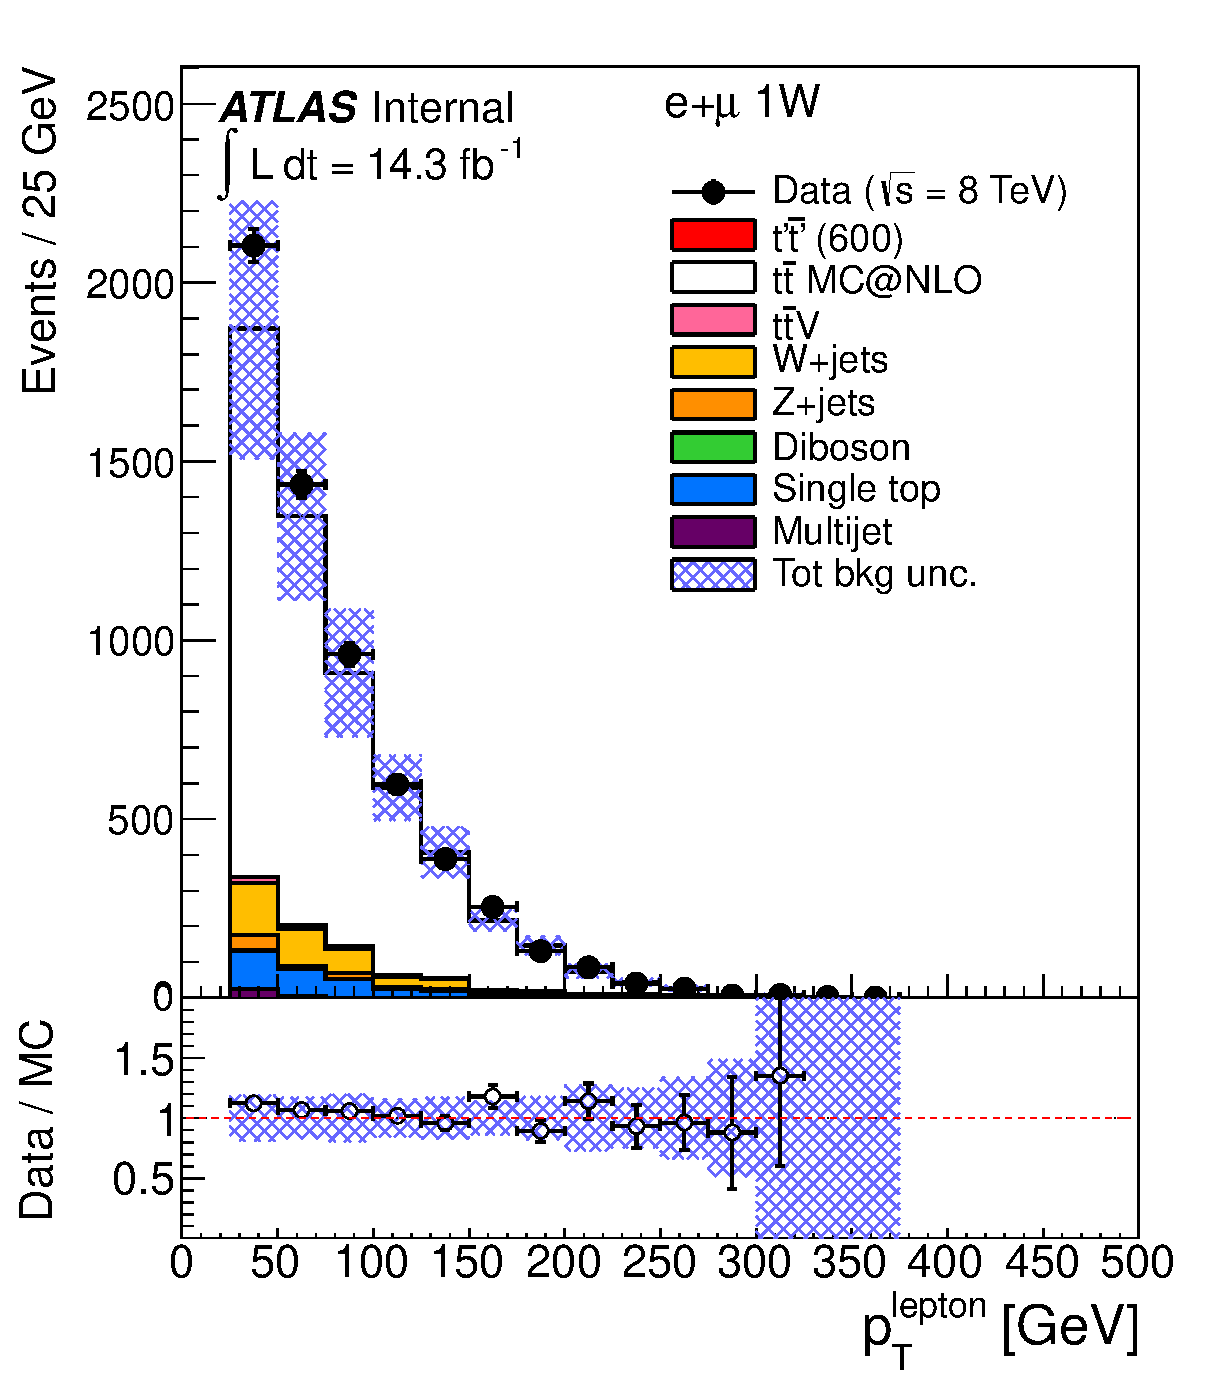
\includegraphics[width=0.30\textwidth]{appendices/figures/sdrs/LepPt_ELEMUONCR0_1W_NOMINAL.eps} &
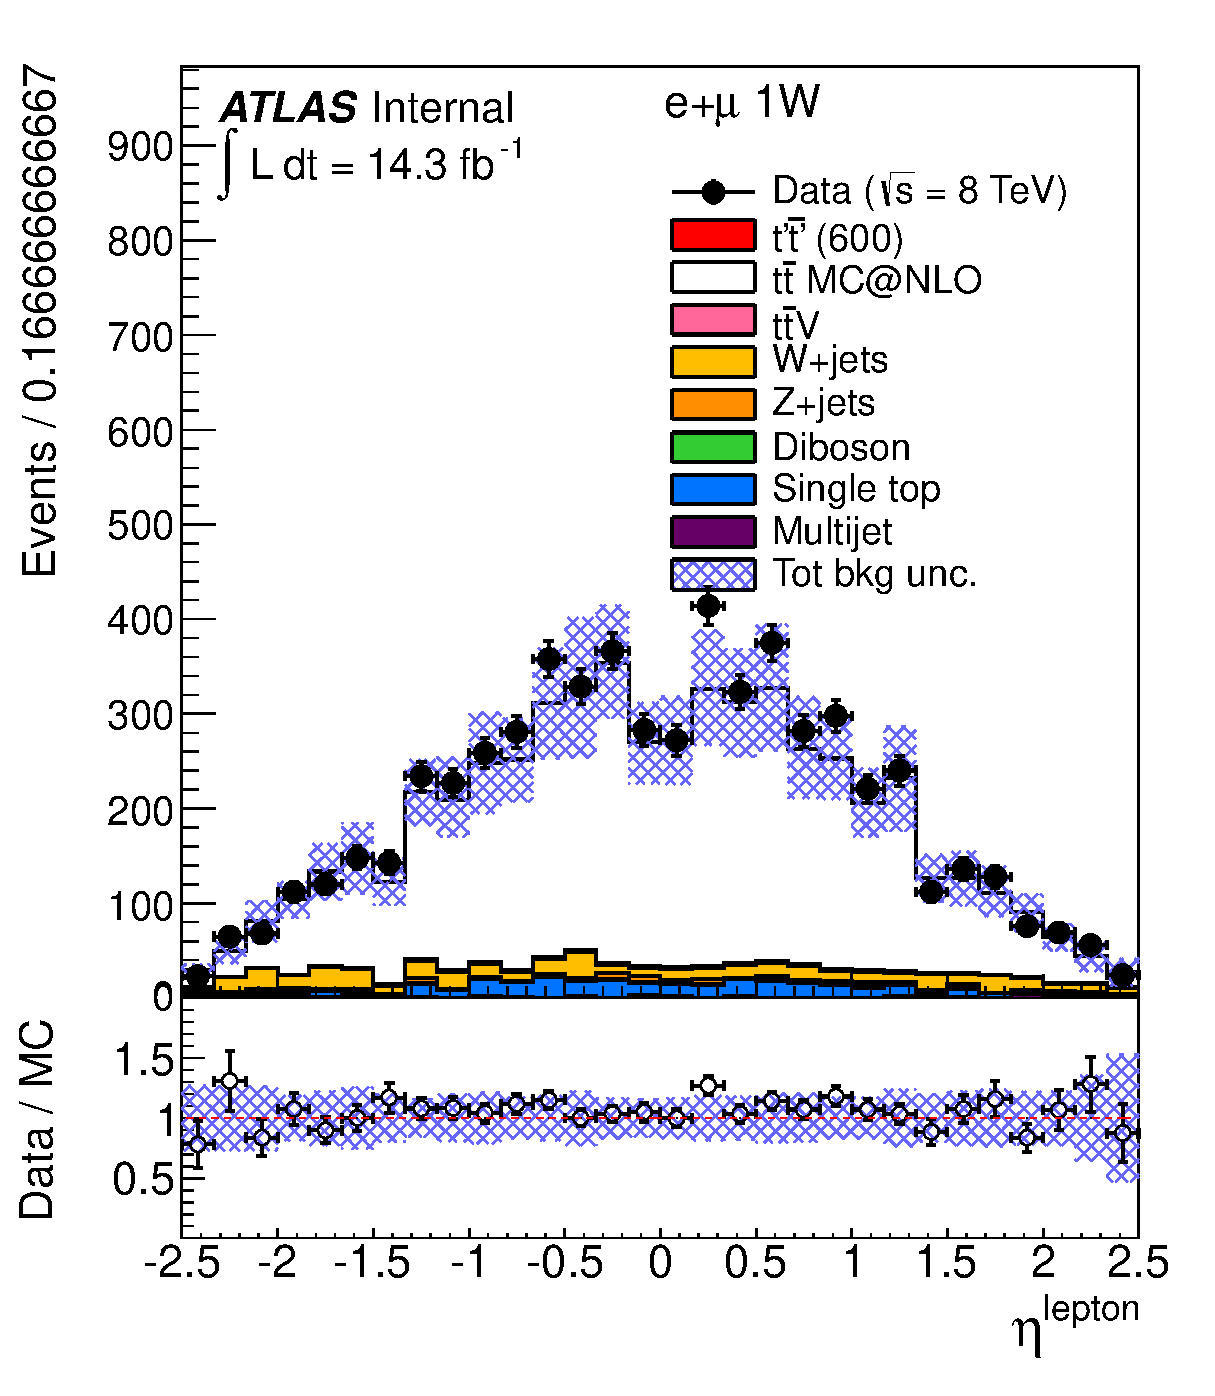
\includegraphics[width=0.30\textwidth]{appendices/figures/sdrs/LepEta_ELEMUONCR0_1W_NOMINAL.eps} &
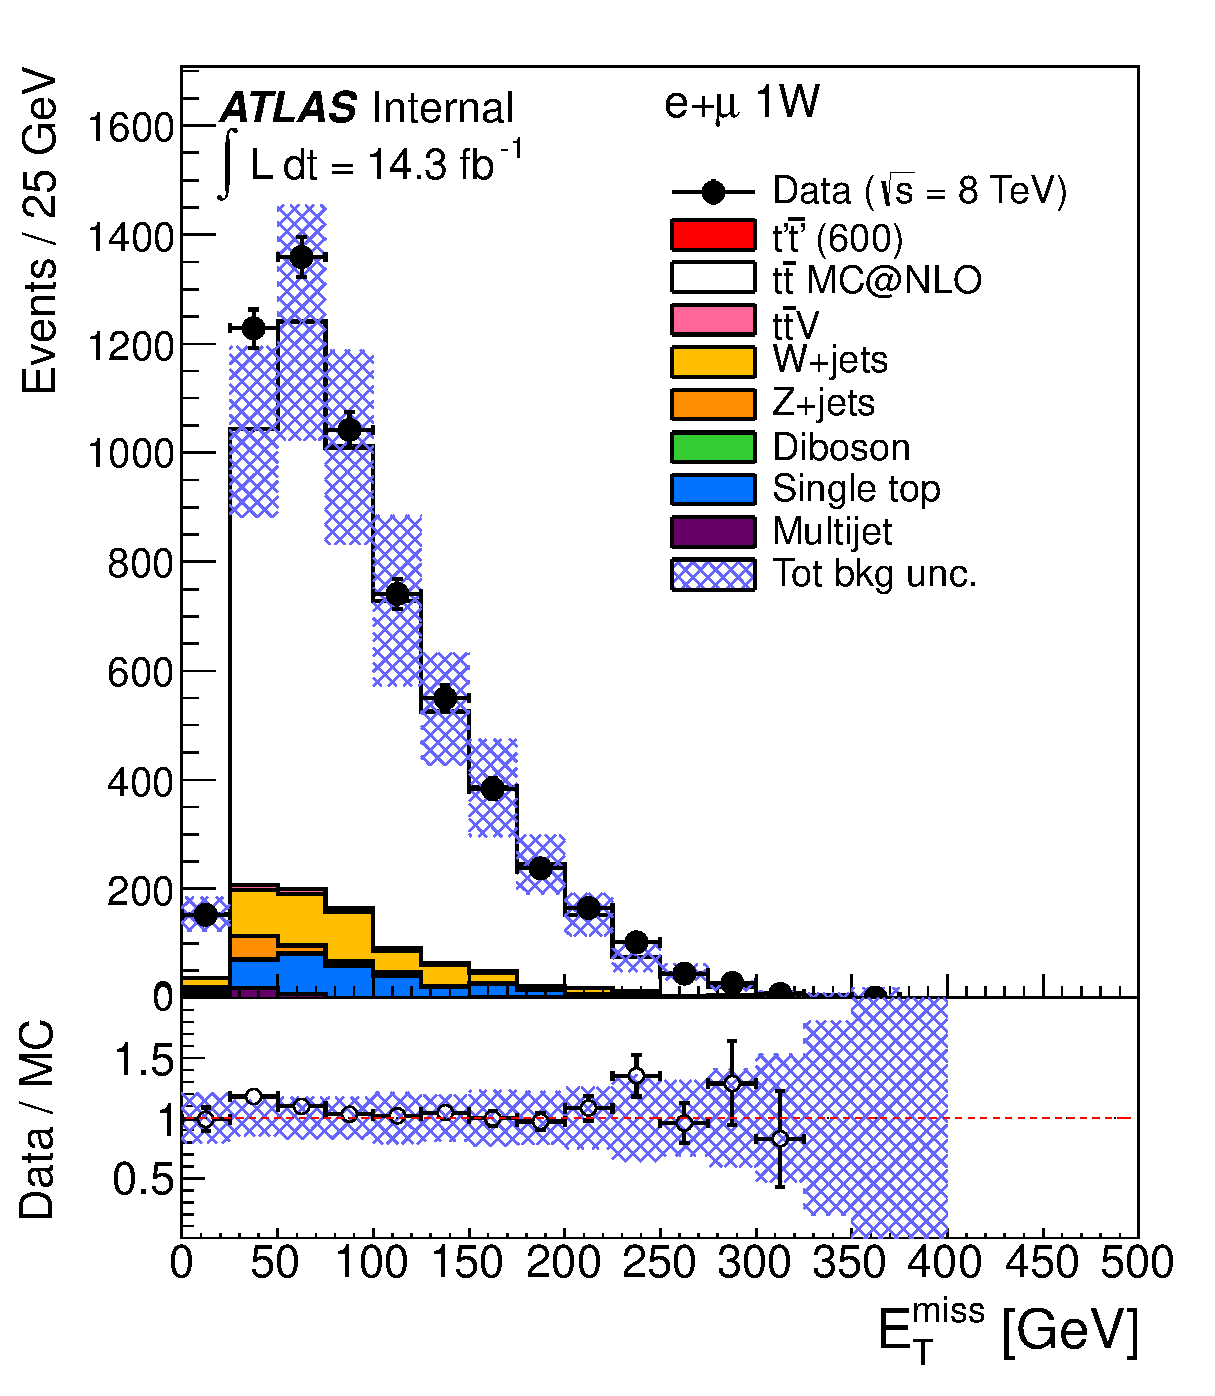
\includegraphics[width=0.30\textwidth]{appendices/figures/sdrs/MET_ELEMUONCR0_1W_NOMINAL.eps} \\
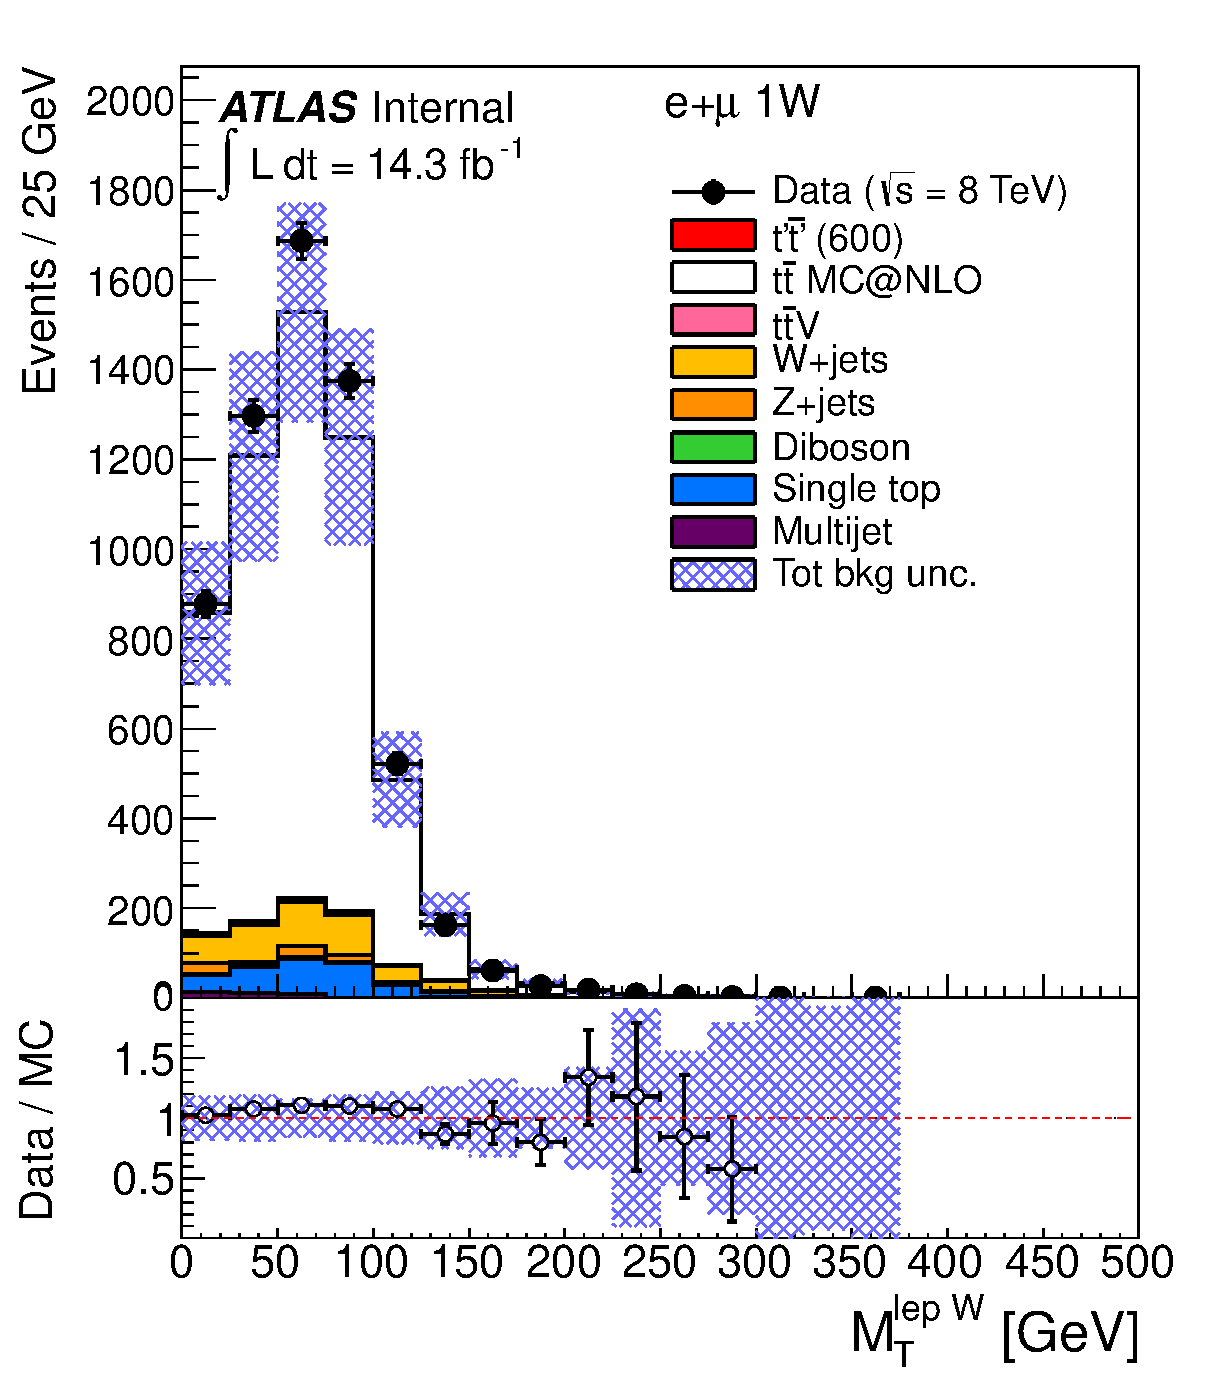
\includegraphics[width=0.30\textwidth]{appendices/figures/sdrs/Wlep_MassT_ELEMUONCR0_1W_NOMINAL.eps} &
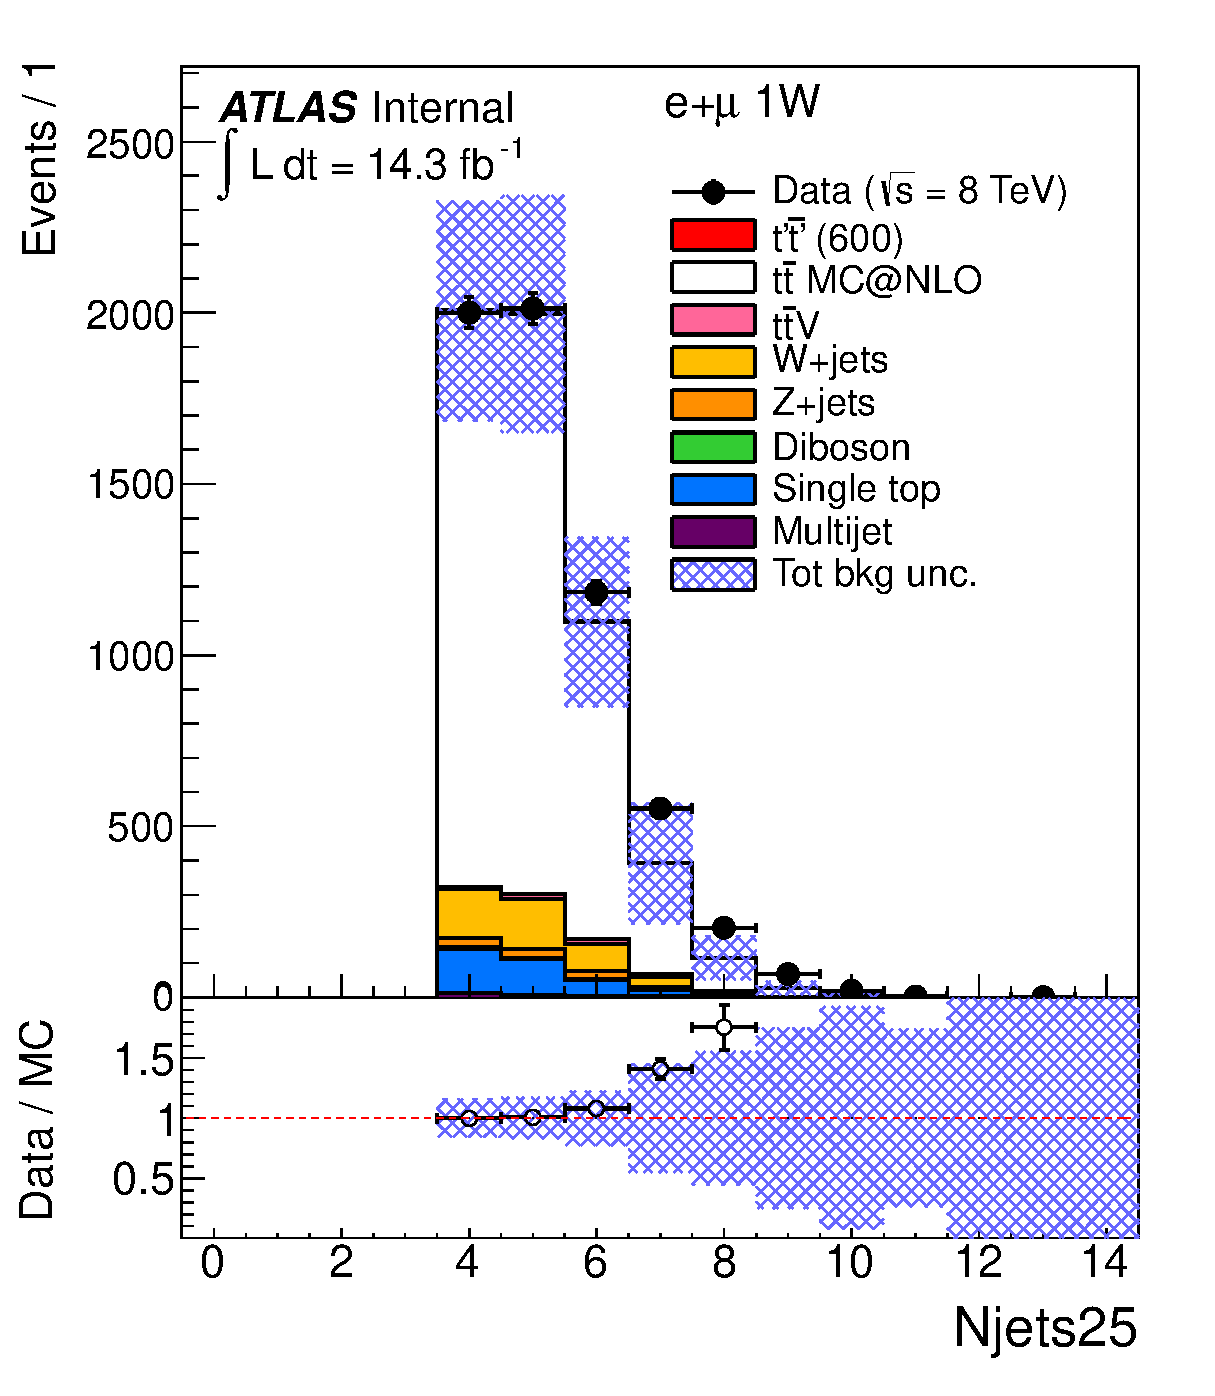
\includegraphics[width=0.30\textwidth]{appendices/figures/sdrs/Njets25_ELEMUONCR0_1W_NOMINAL.eps}  &
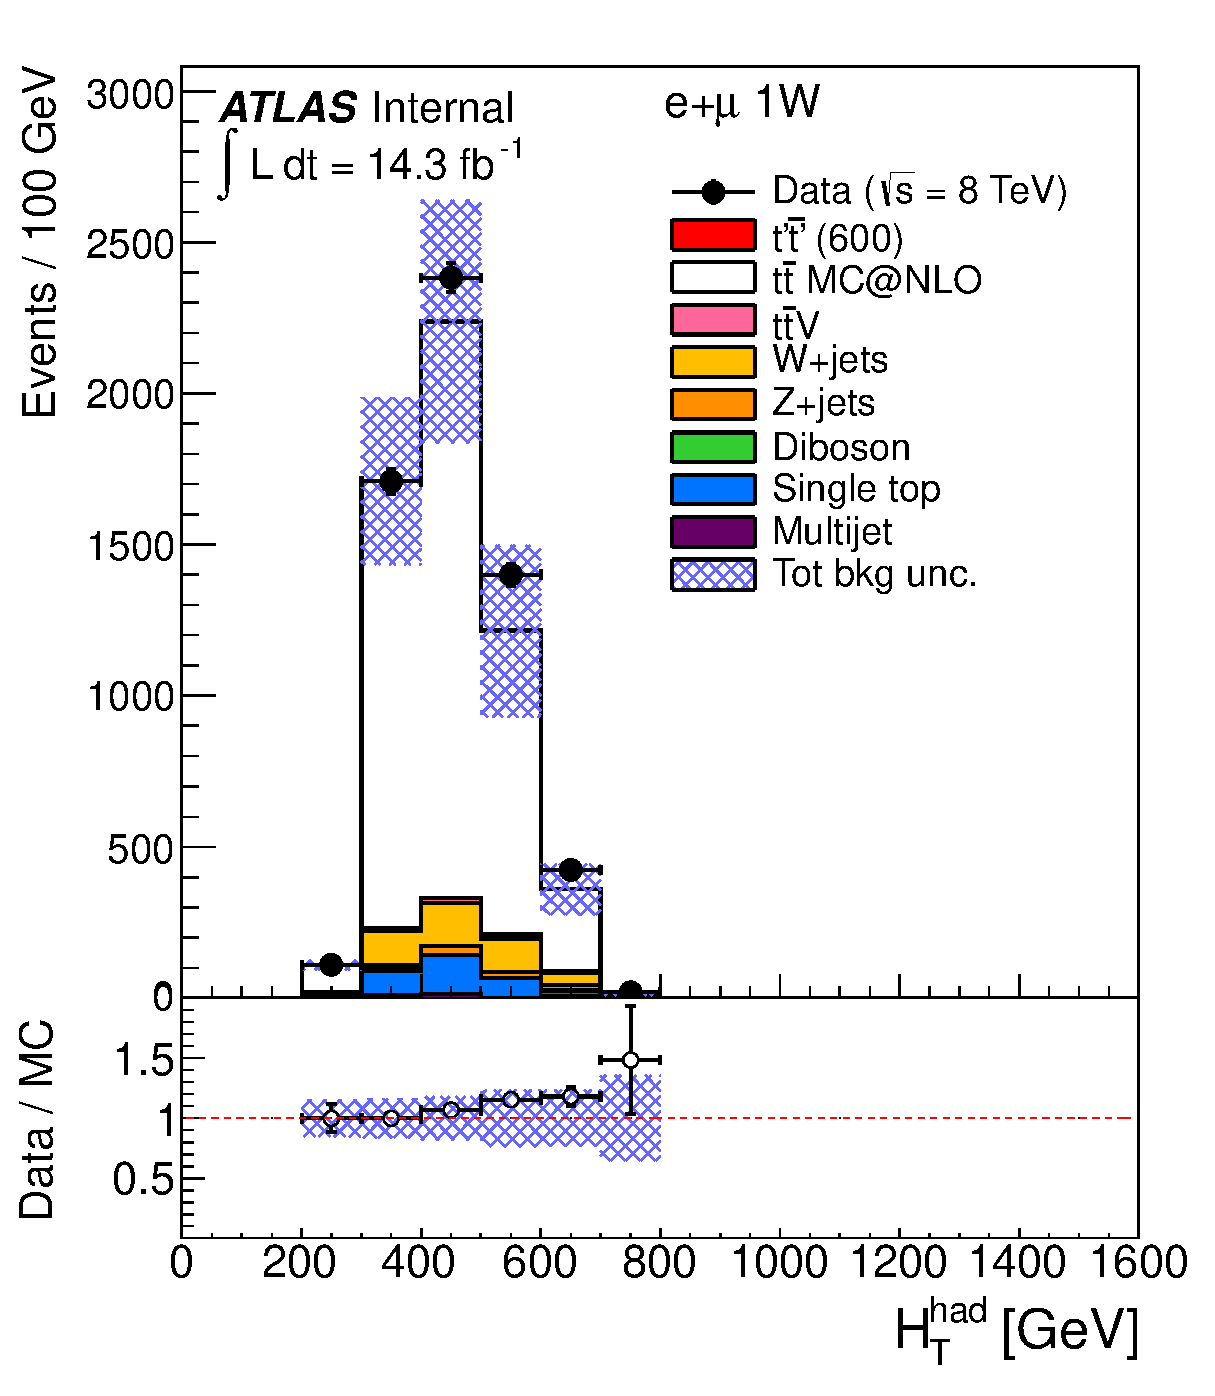
\includegraphics[width=0.30\textwidth]{appendices/figures/sdrs/HTHad_ELEMUONCR0_1W_NOMINAL.eps}  \\
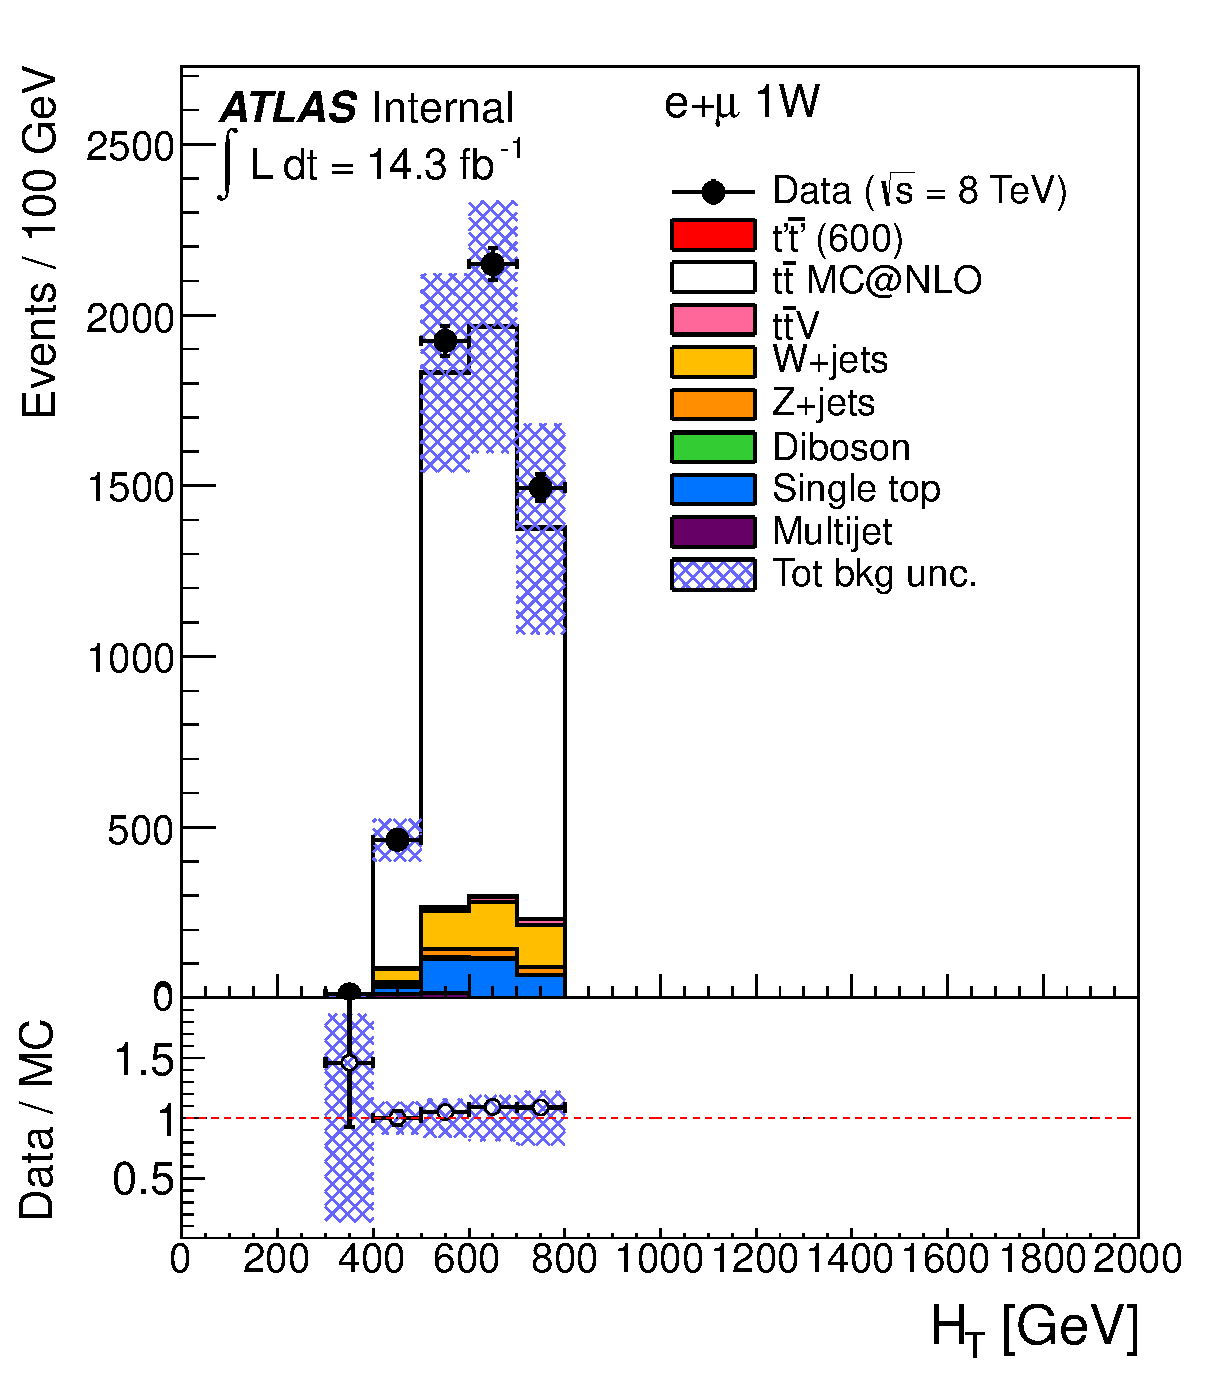
\includegraphics[width=0.30\textwidth]{appendices/figures/sdrs/HTAll_ELEMUONCR0_1W_NOMINAL.eps}  &  &\\
\end{tabular}\caption{\small {Comparison between data and prediction in combined $e$+jets and $\mu$+jets channel in SDR0 (see Sect.~\ref{sec:sdrs} for details) 
for a number of kinematic variables. From top to bottom and left to right, the variables displayed are: lepton $\pt$, lepton $\eta$, missing transverse energy, $W$ transverse mass,
$\hthad$, and $\HT$. The shaded area represents the total background uncertainty.}}
\label{fig:ELEMUONCR0_1}
\end{center}
\end{figure}                                                                             
%%%%%%%%%%%%%%

\clearpage
%%%%%%%%%%%%%%
\begin{figure}[htbp]
\begin{center}
\begin{tabular}{cc}
%
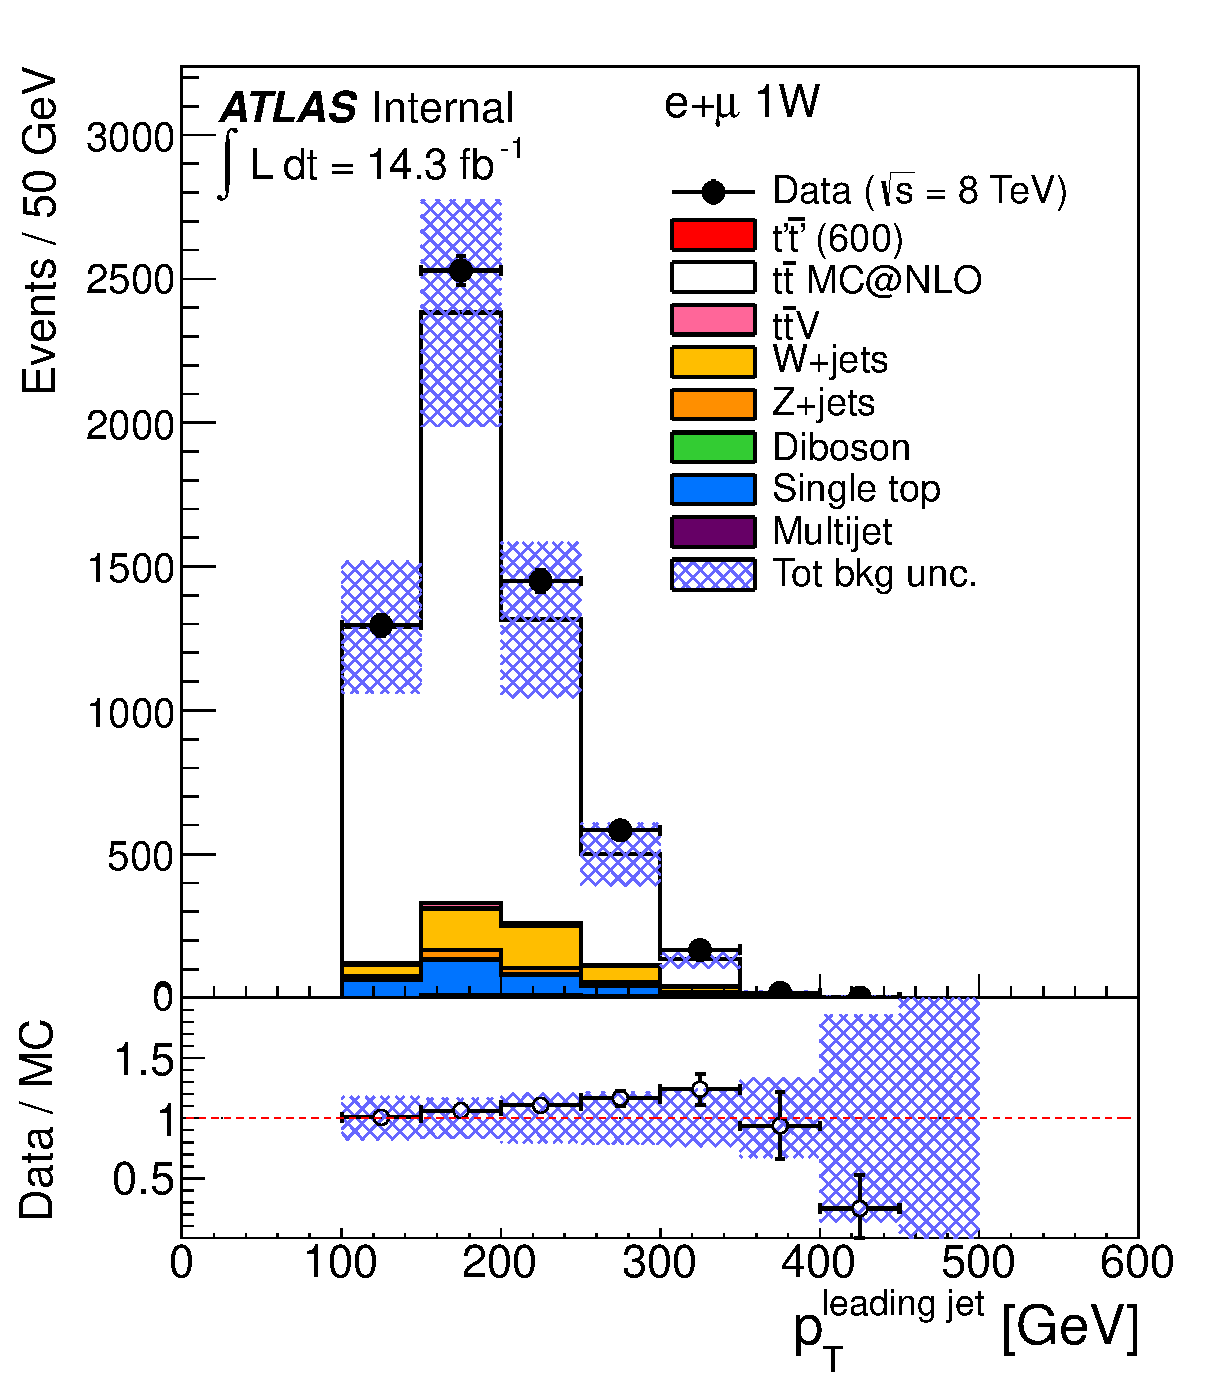
\includegraphics[width=0.30\textwidth]{appendices/figures/sdrs/JetPt1_ELEMUONCR0_1W_NOMINAL.eps} &
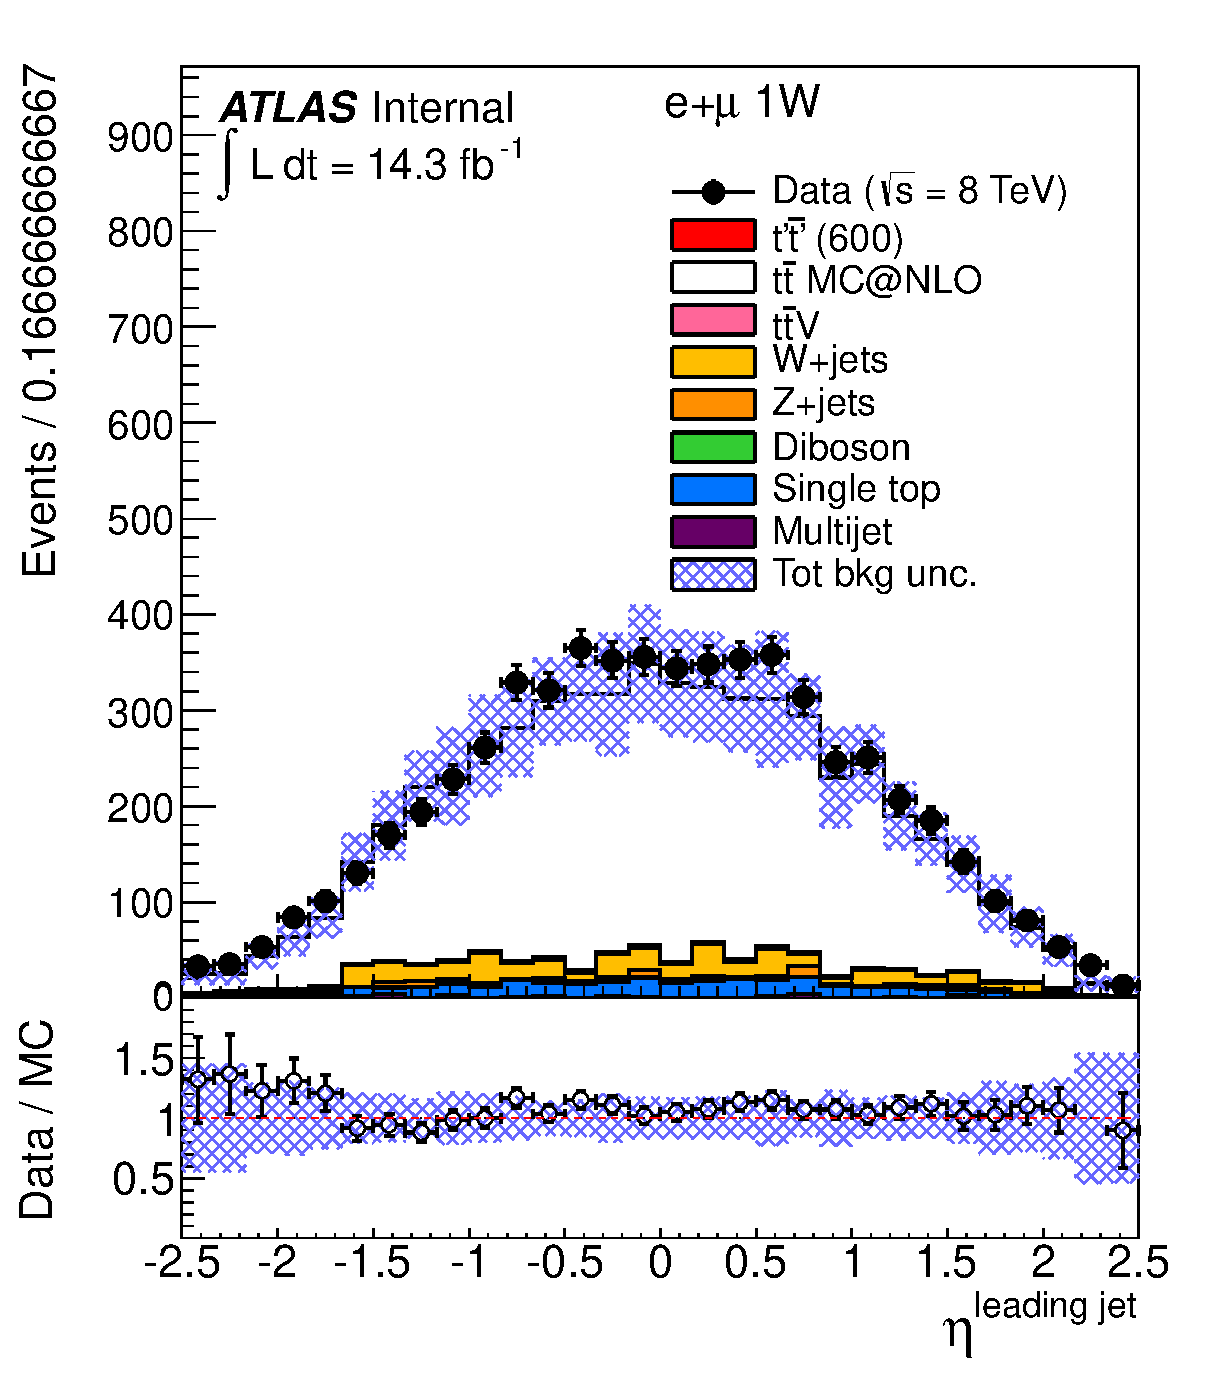
\includegraphics[width=0.30\textwidth]{appendices/figures/sdrs/JetEta1_ELEMUONCR0_1W_NOMINAL.eps} \\
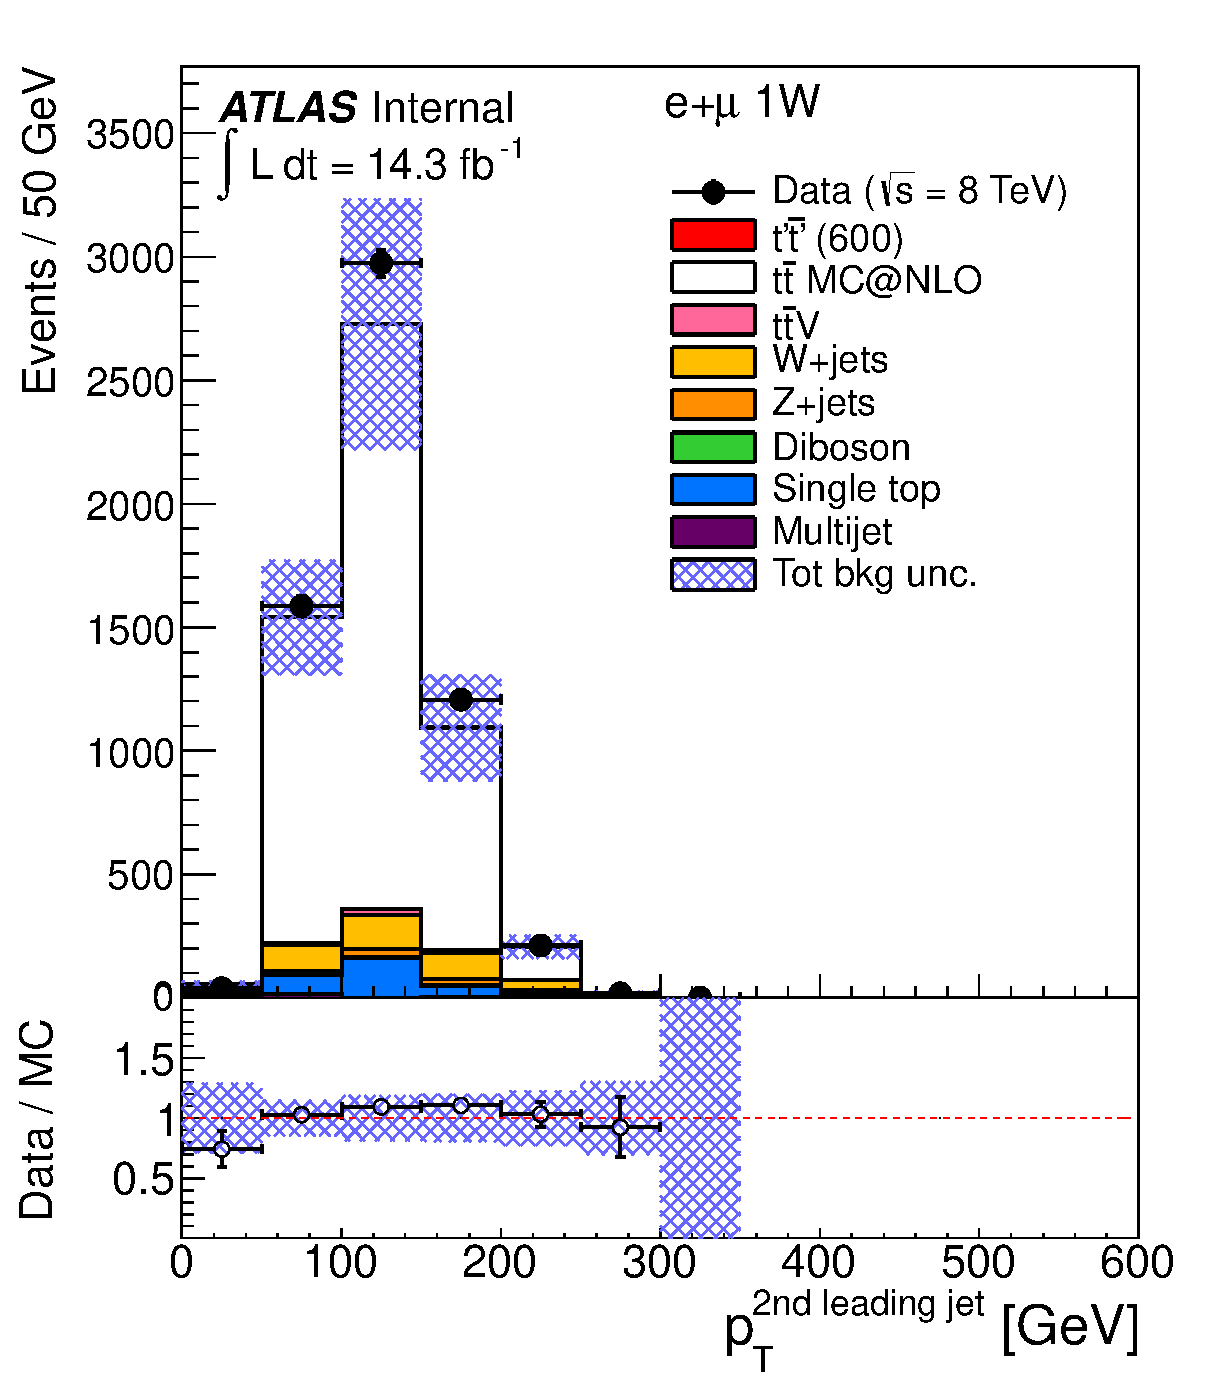
\includegraphics[width=0.30\textwidth]{appendices/figures/sdrs/JetPt2_ELEMUONCR0_1W_NOMINAL.eps} &
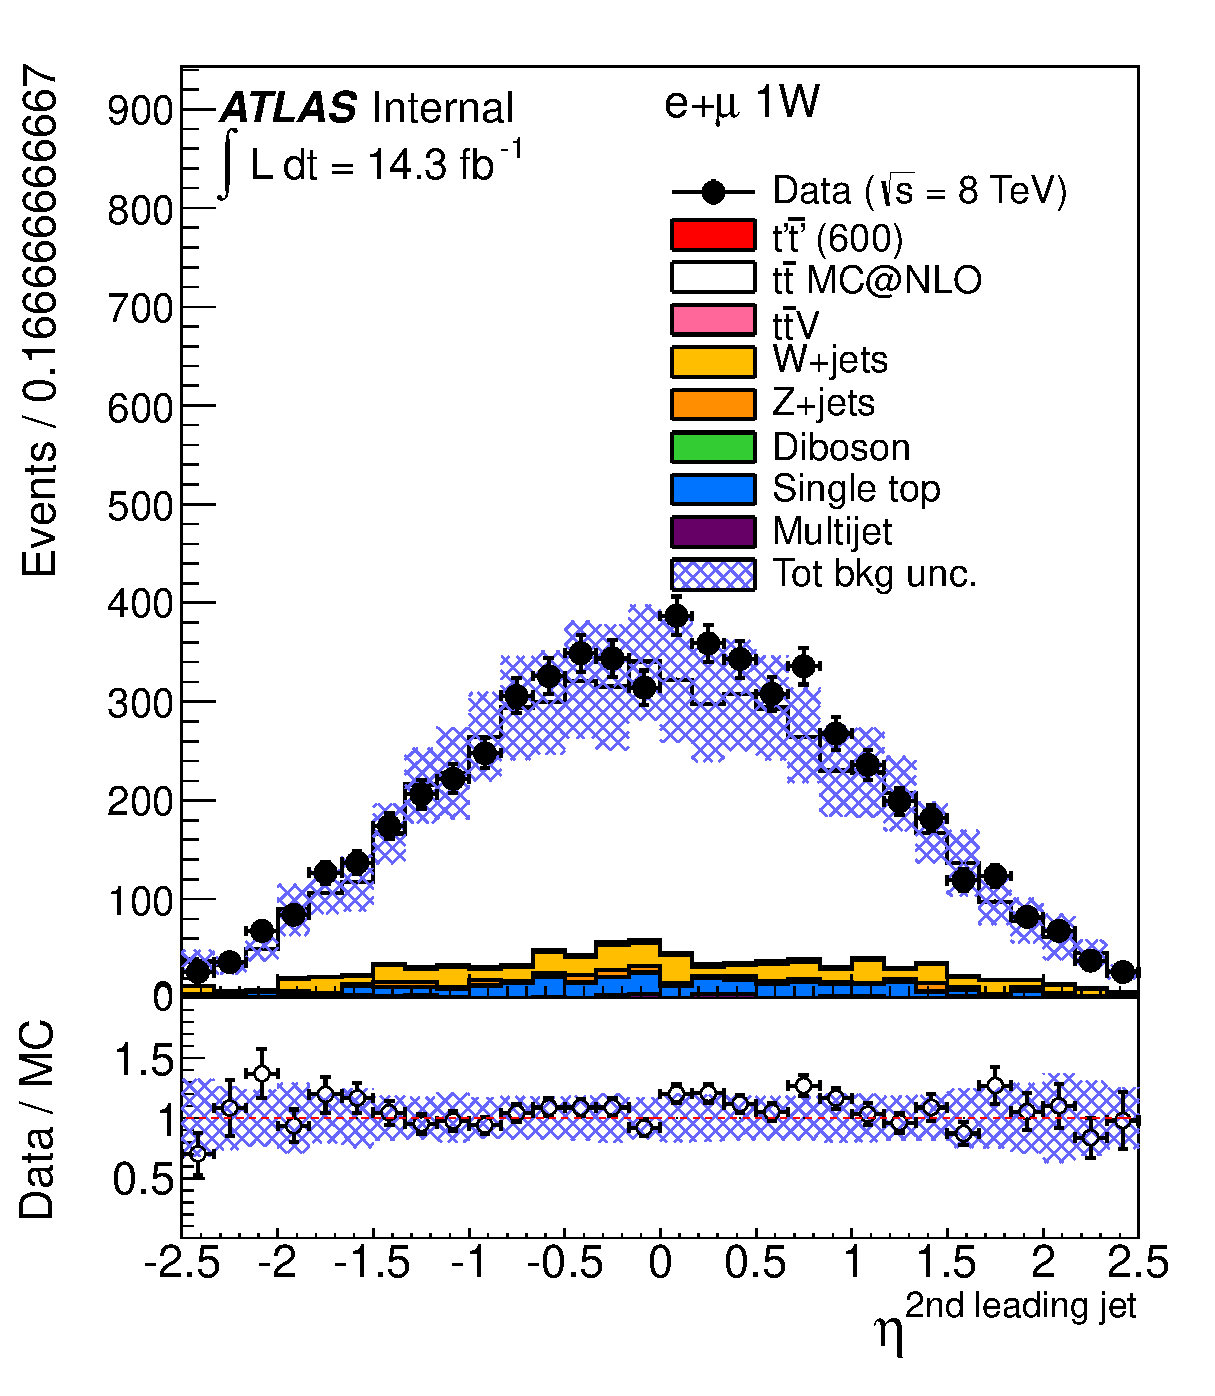
\includegraphics[width=0.30\textwidth]{appendices/figures/sdrs/JetEta2_ELEMUONCR0_1W_NOMINAL.eps} \\
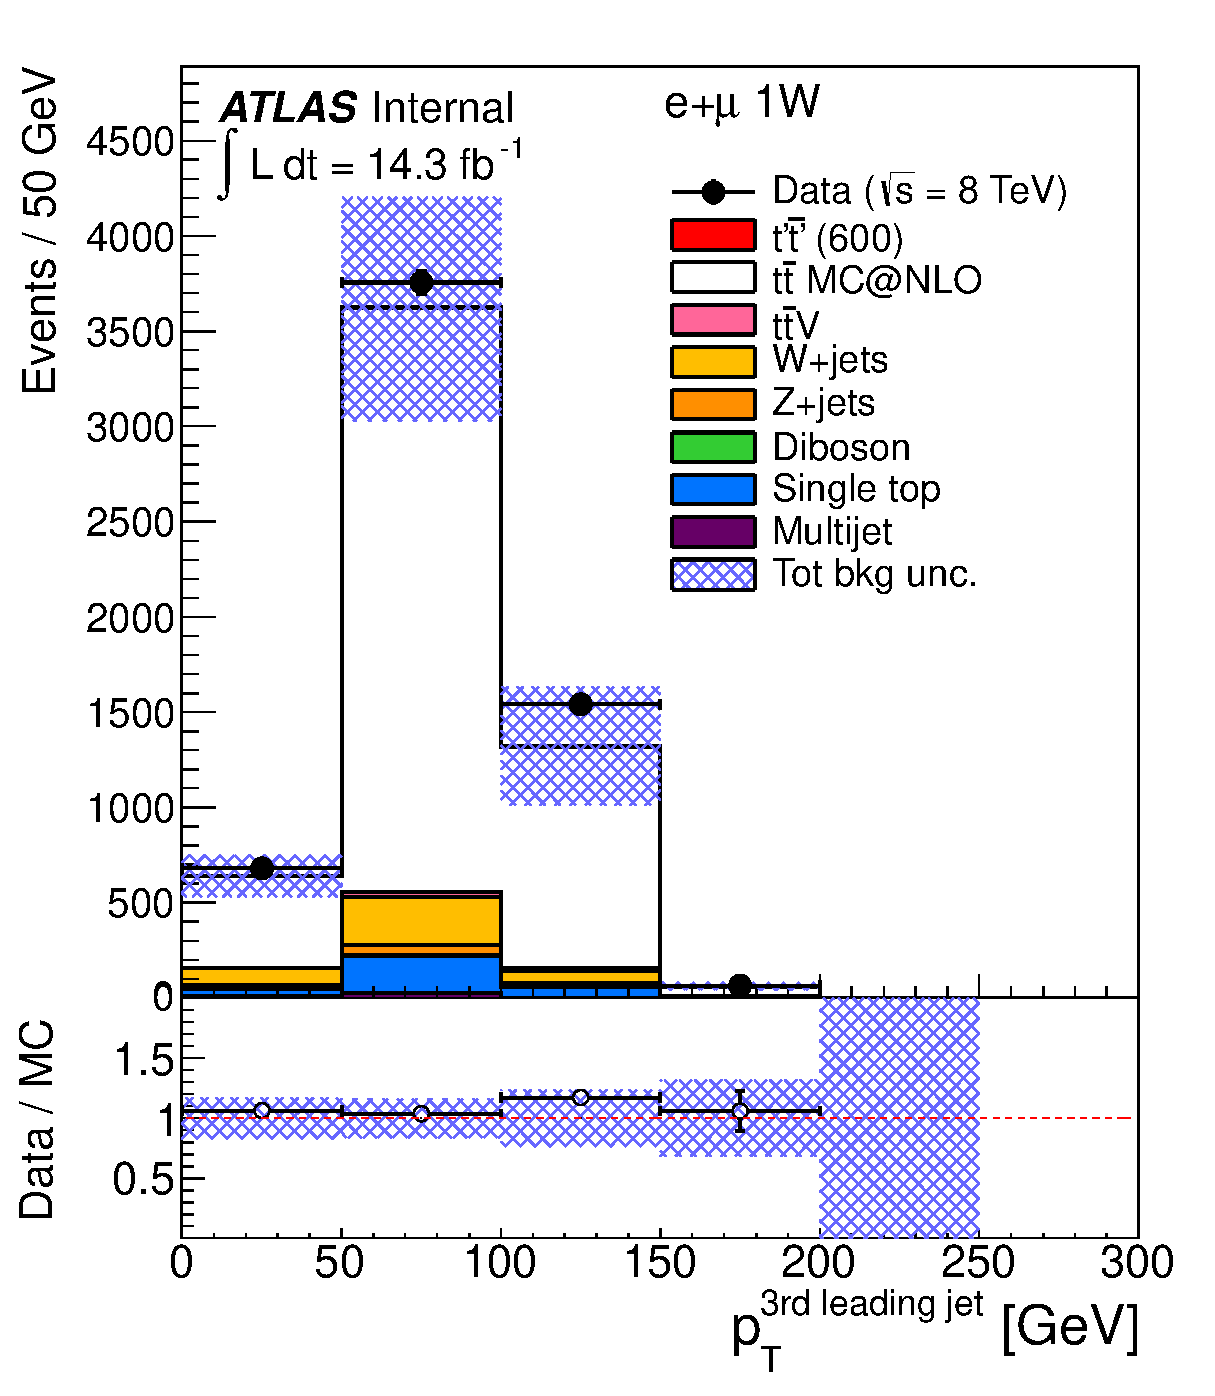
\includegraphics[width=0.30\textwidth]{appendices/figures/sdrs/JetPt3_ELEMUONCR0_1W_NOMINAL.eps} &
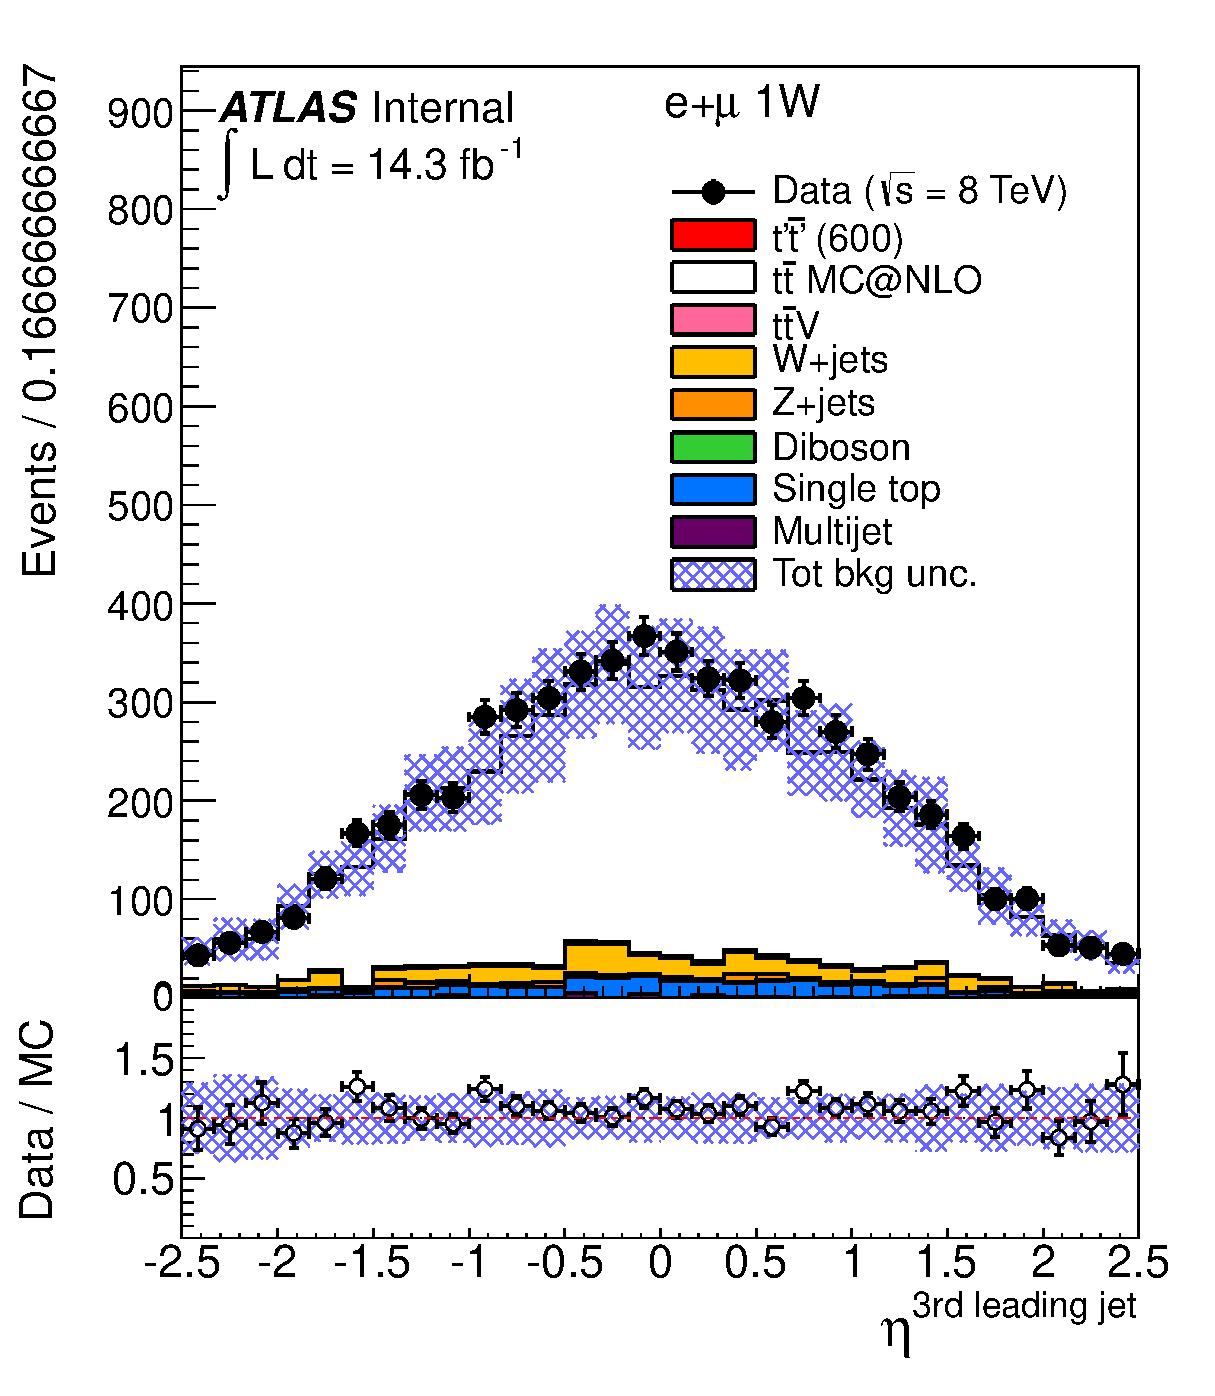
\includegraphics[width=0.30\textwidth]{appendices/figures/sdrs/JetEta3_ELEMUONCR0_1W_NOMINAL.eps} \\
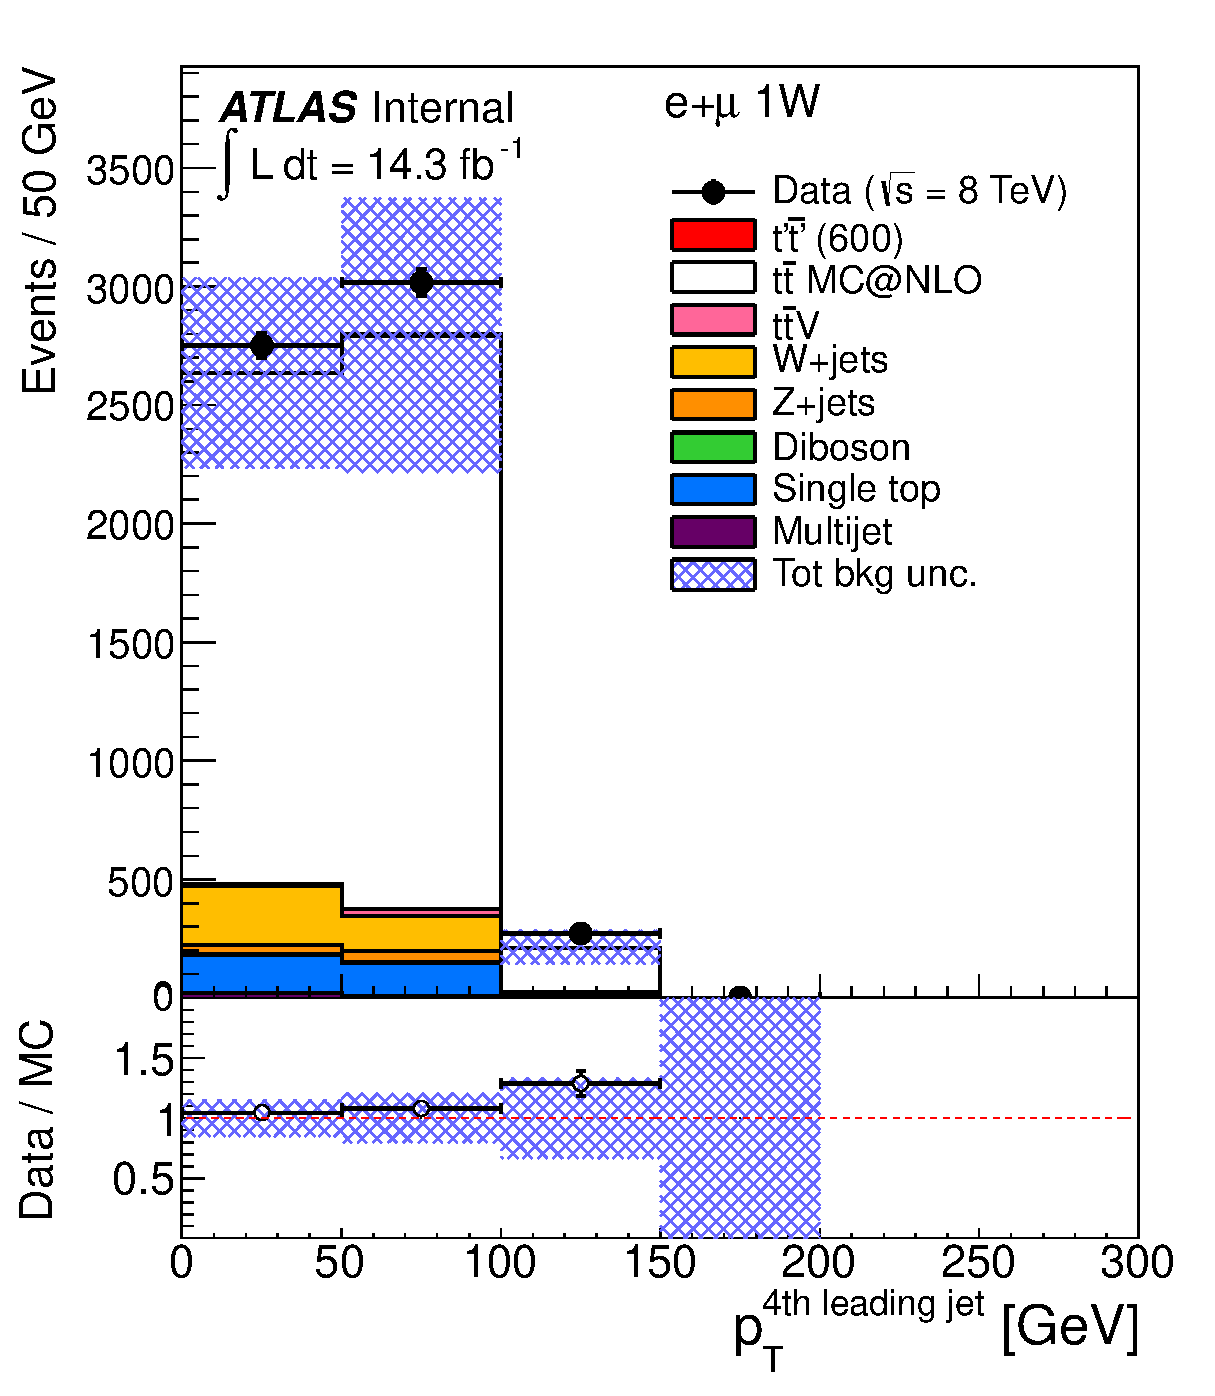
\includegraphics[width=0.30\textwidth]{appendices/figures/sdrs/JetPt4_ELEMUONCR0_1W_NOMINAL.eps}  &
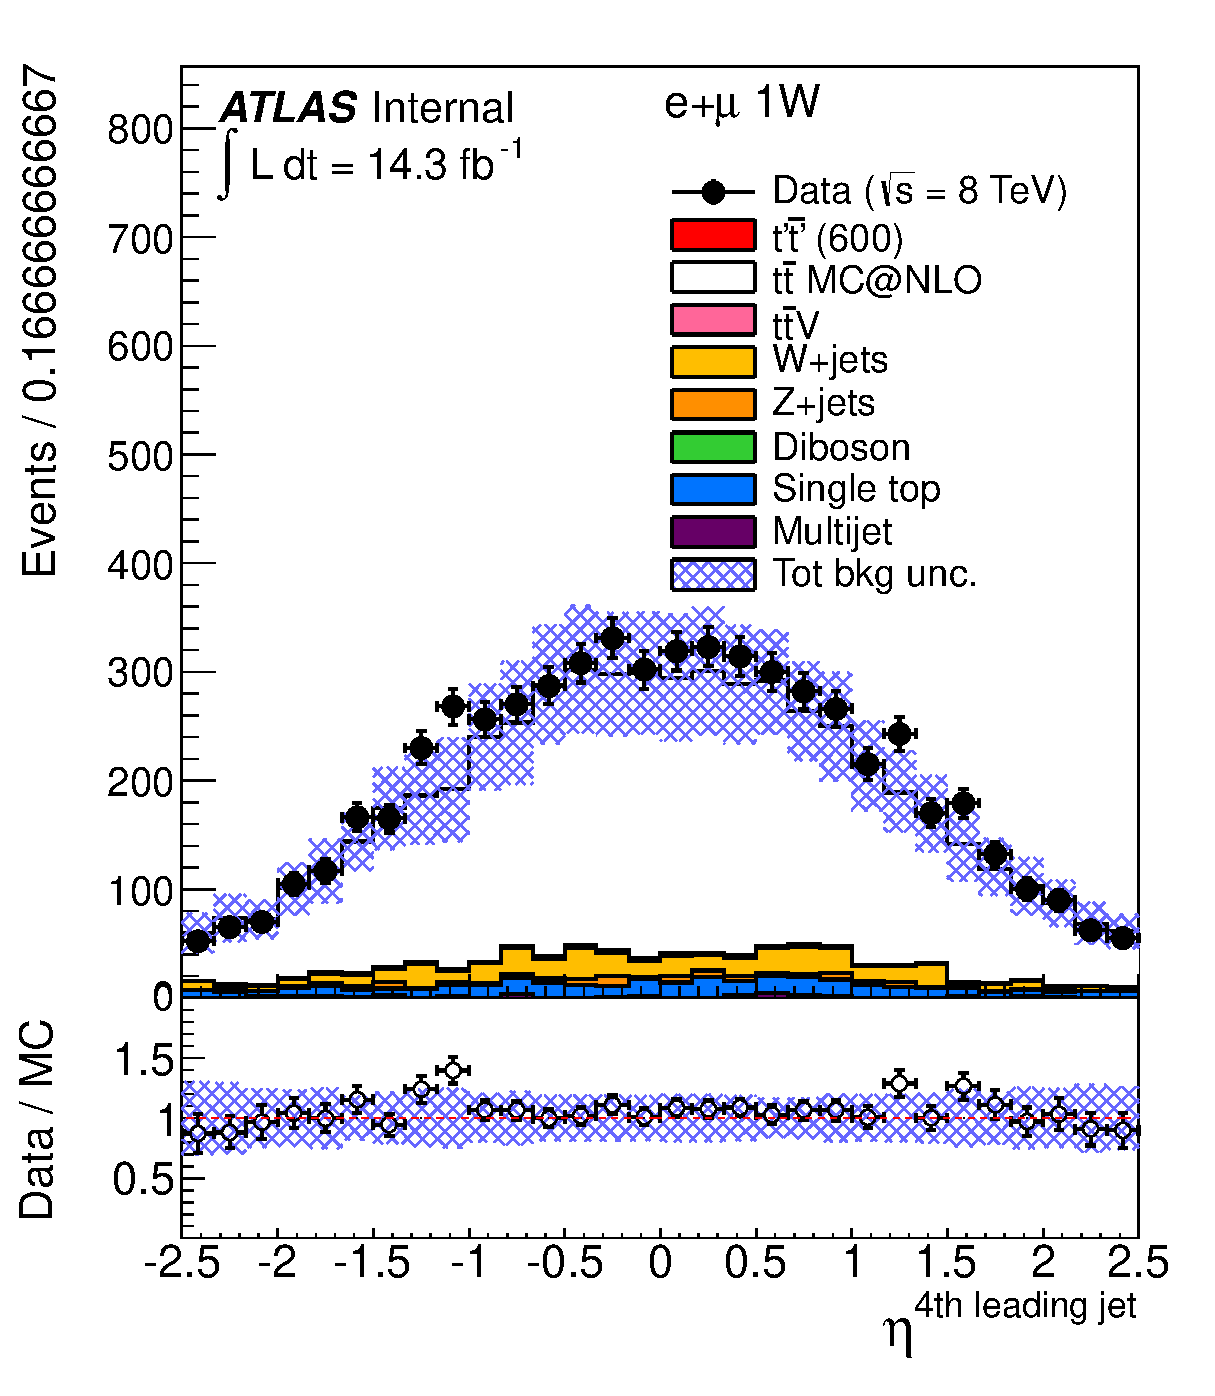
\includegraphics[width=0.30\textwidth]{appendices/figures/sdrs/JetEta4_ELEMUONCR0_1W_NOMINAL.eps}  \\
\end{tabular}\caption{\small {Comparison between data and prediction in combined $e$+jets and $\mu$+jets channel in SDR0 (see Sect.~\ref{sec:sdrs} for details) 
for a number of kinematic variables. From top to bottom and left to right, the variables displayed are: leading jet $\pt$ and $\eta$,  second leading jet $\pt$ and $\eta$,
third leading jet $\pt$ and $\eta$, and fourth leading jet $\pt$ and $\eta$. The shaded area represents the total background uncertainty.}}
\label{fig:ELEMUONCR0_2}
\end{center}
\end{figure}                                                                             
%%%%%%%%%%%%%%

\clearpage
%%%%%%%%%%%%%%
\begin{figure}[htbp]
\begin{center}
\begin{tabular}{ccc}
%
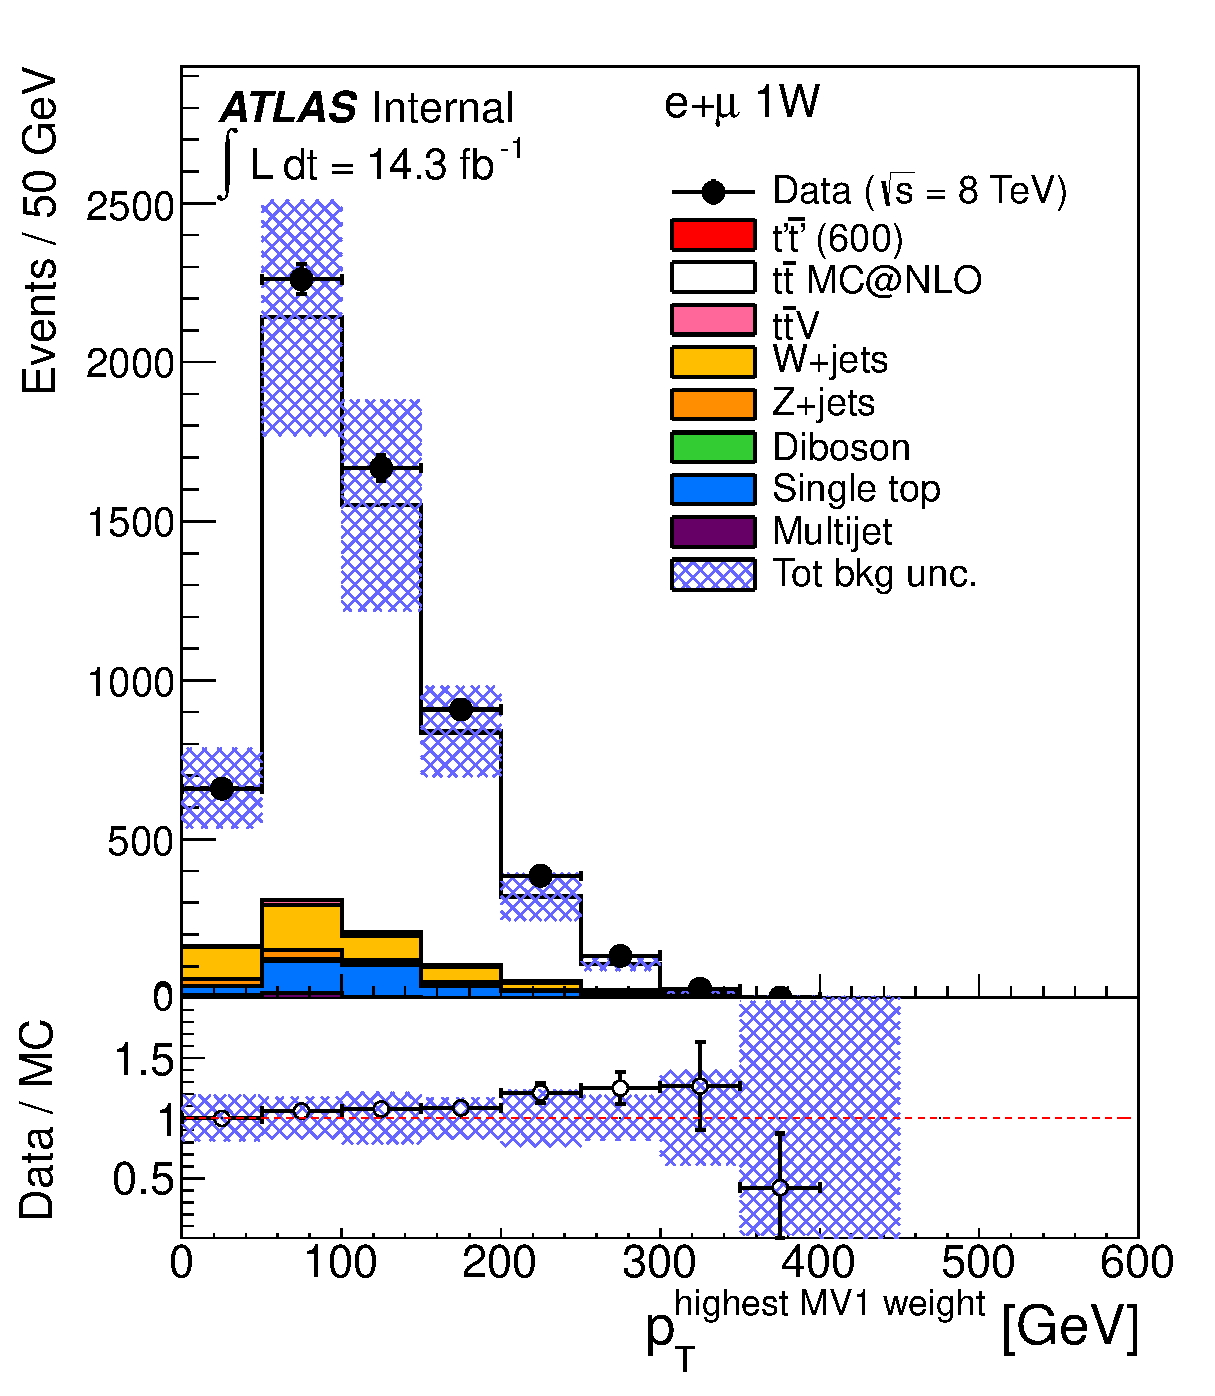
\includegraphics[width=0.30\textwidth]{appendices/figures/sdrs/JetPtB1_ELEMUONCR0_1W_NOMINAL.eps}  &
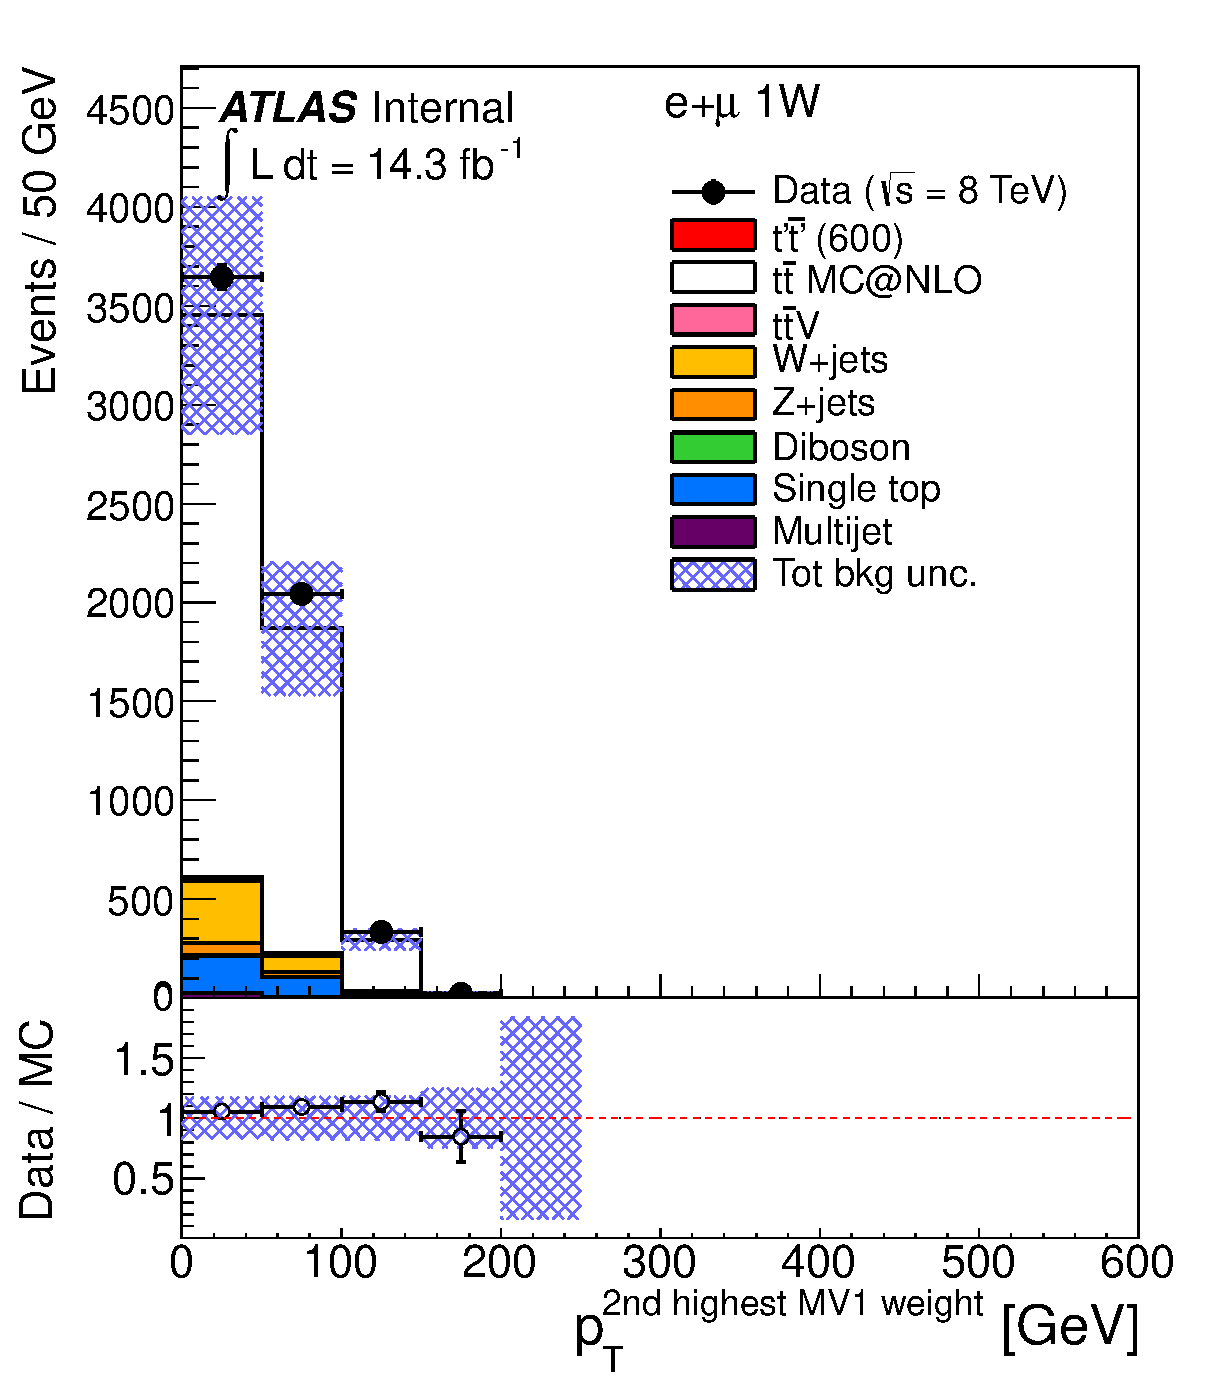
\includegraphics[width=0.30\textwidth]{appendices/figures/sdrs/JetPtB2_ELEMUONCR0_1W_NOMINAL.eps} &
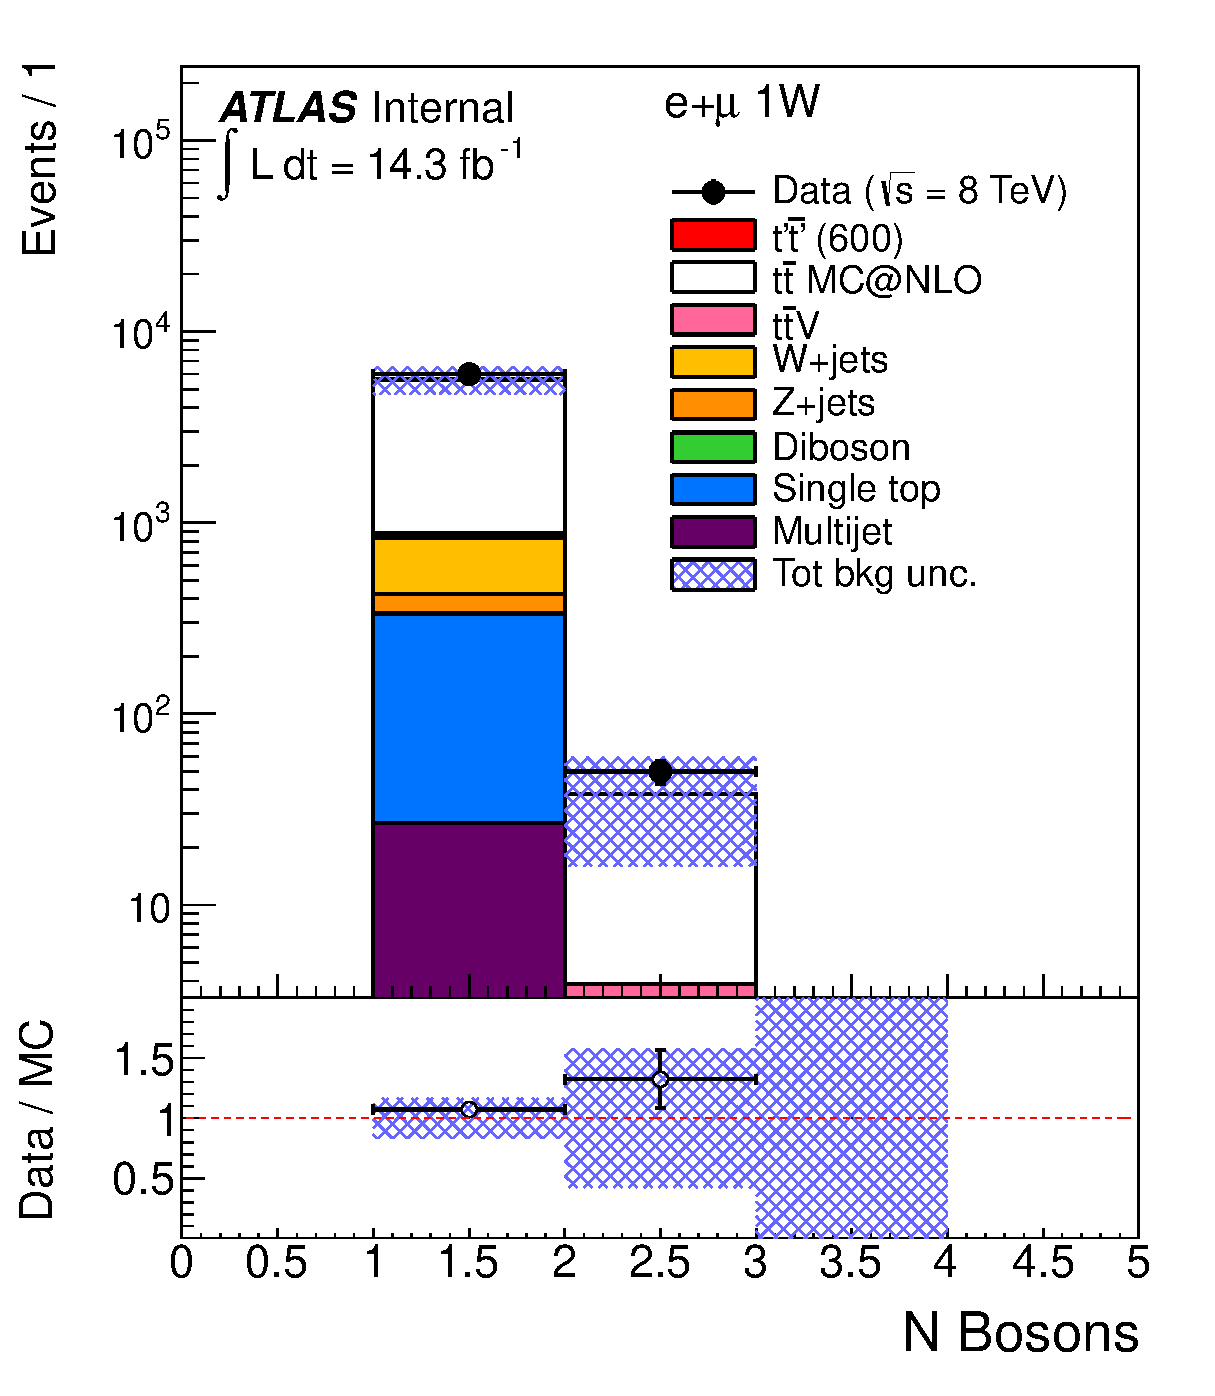
\includegraphics[width=0.30\textwidth]{appendices/figures/sdrs/nWhad_ELEMUONCR0_1W_NOMINAL_logscale.eps} \\
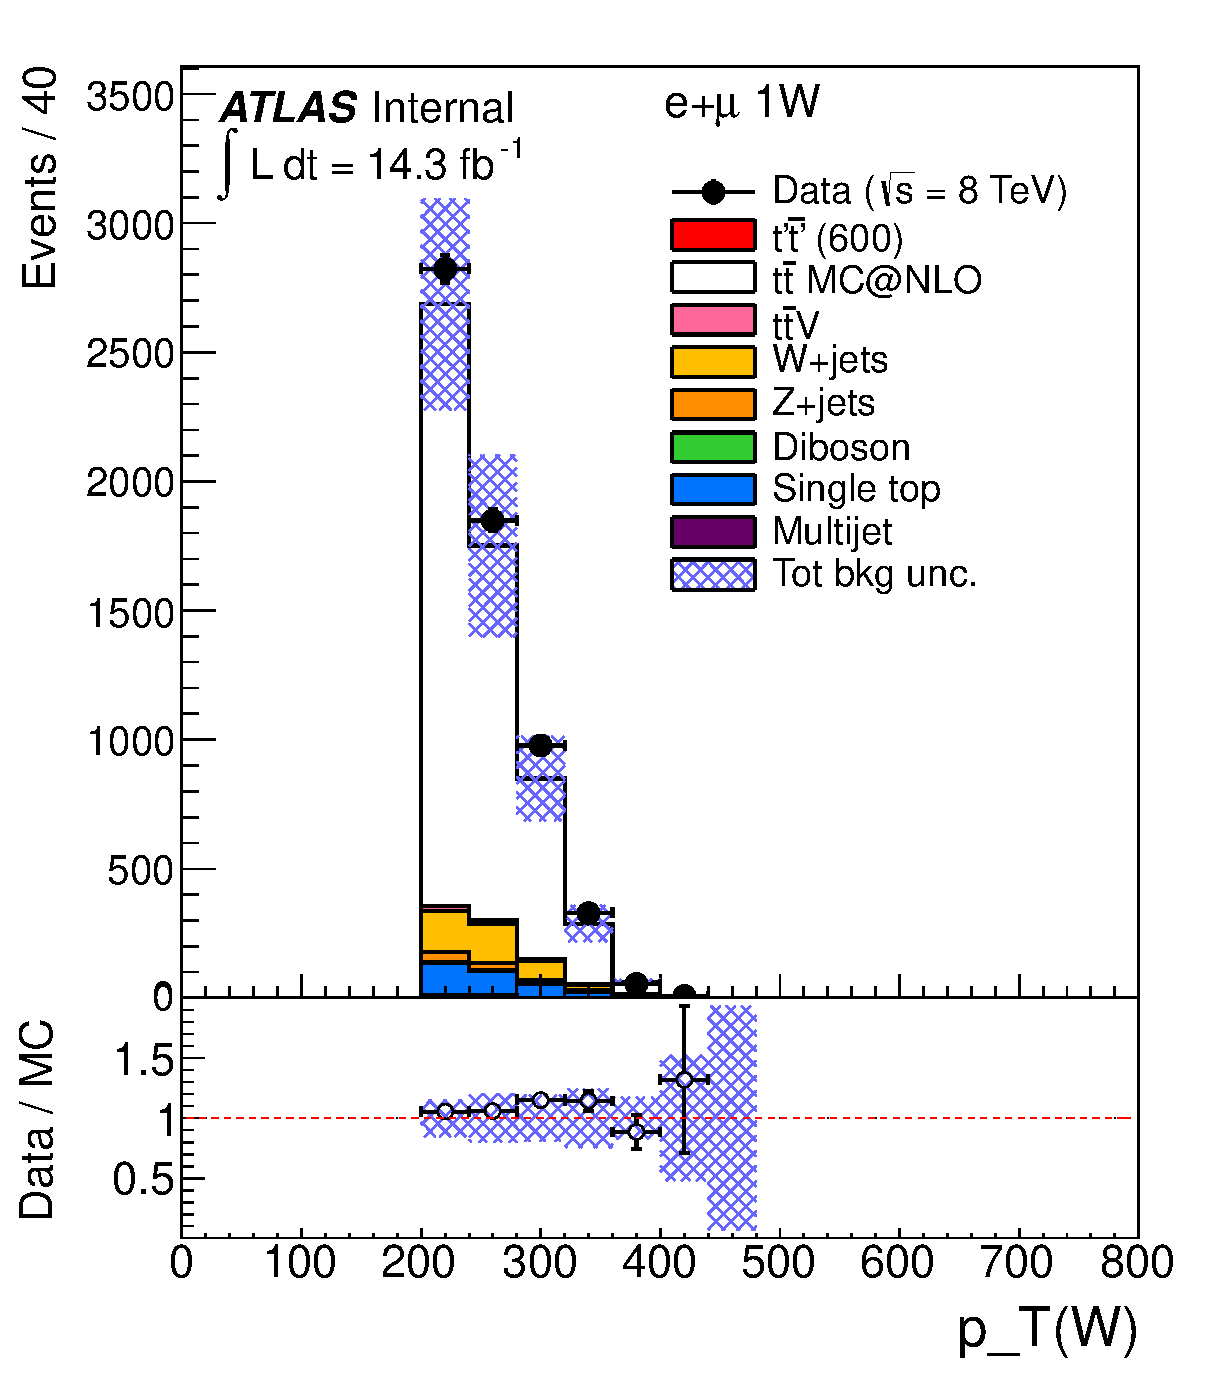
\includegraphics[width=0.30\textwidth]{appendices/figures/sdrs/VLQAna_WbX_W1Pt_ELEMUONCR0_1W_NOMINAL.eps} &
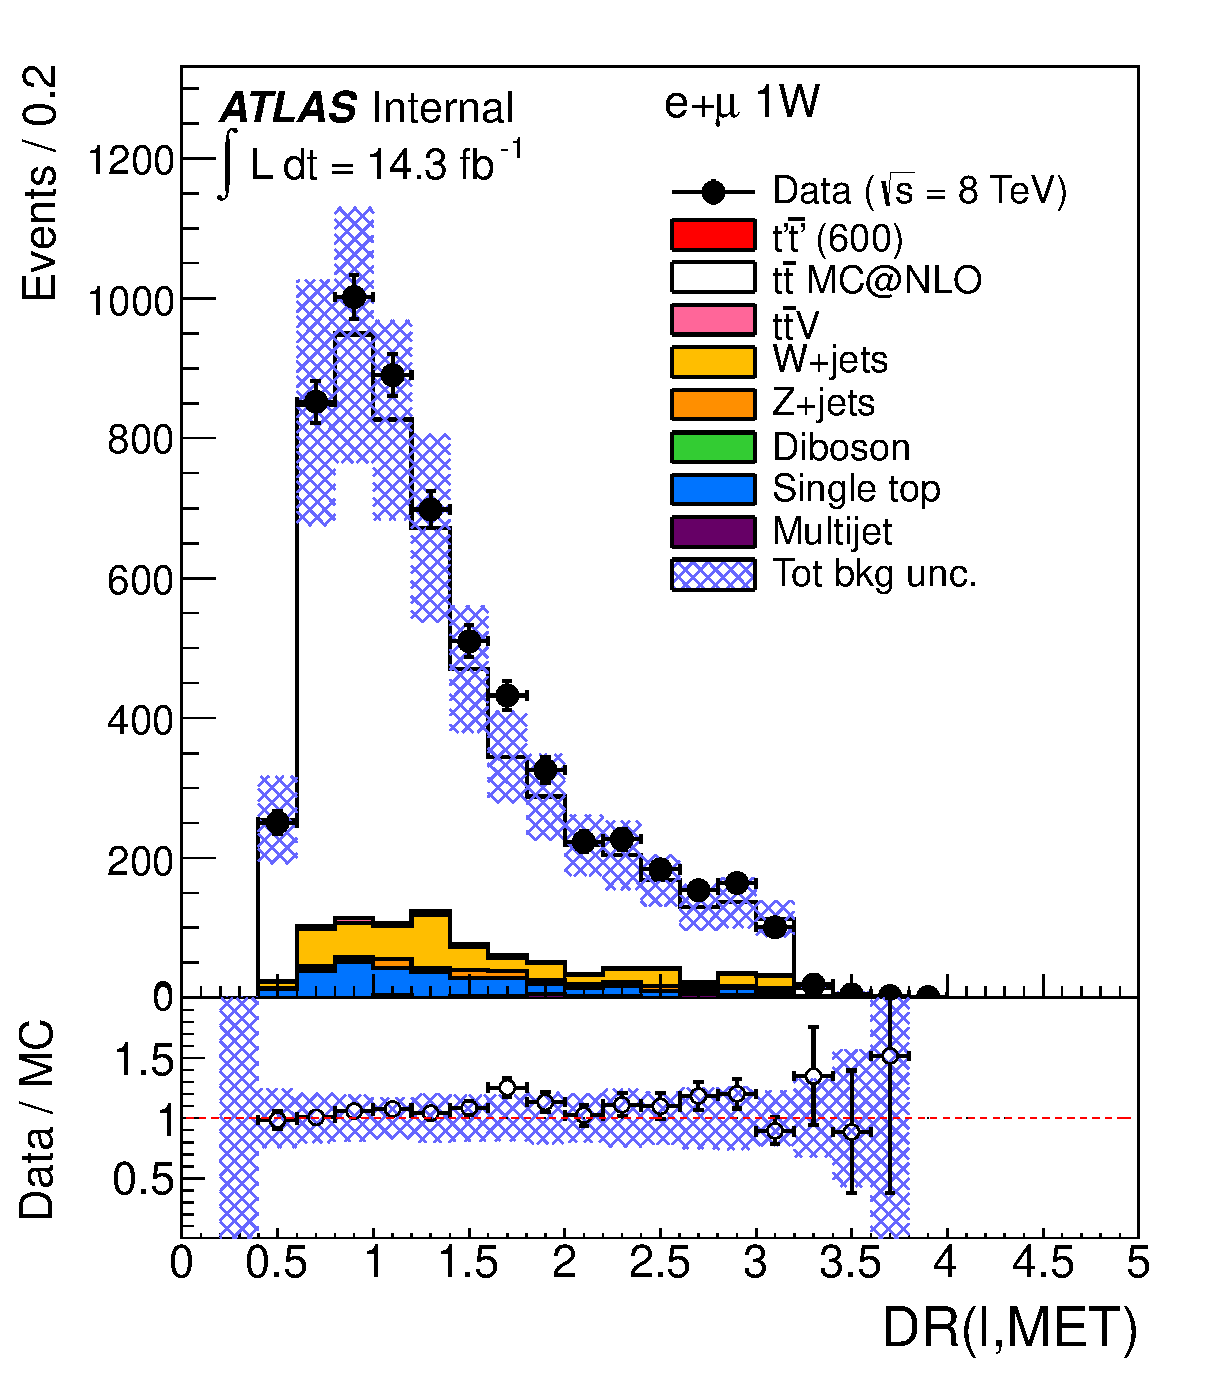
\includegraphics[width=0.30\textwidth]{appendices/figures/sdrs/VLQAna_WbX_DRLepMet_ELEMUONCR0_1W_NOMINAL.eps} &
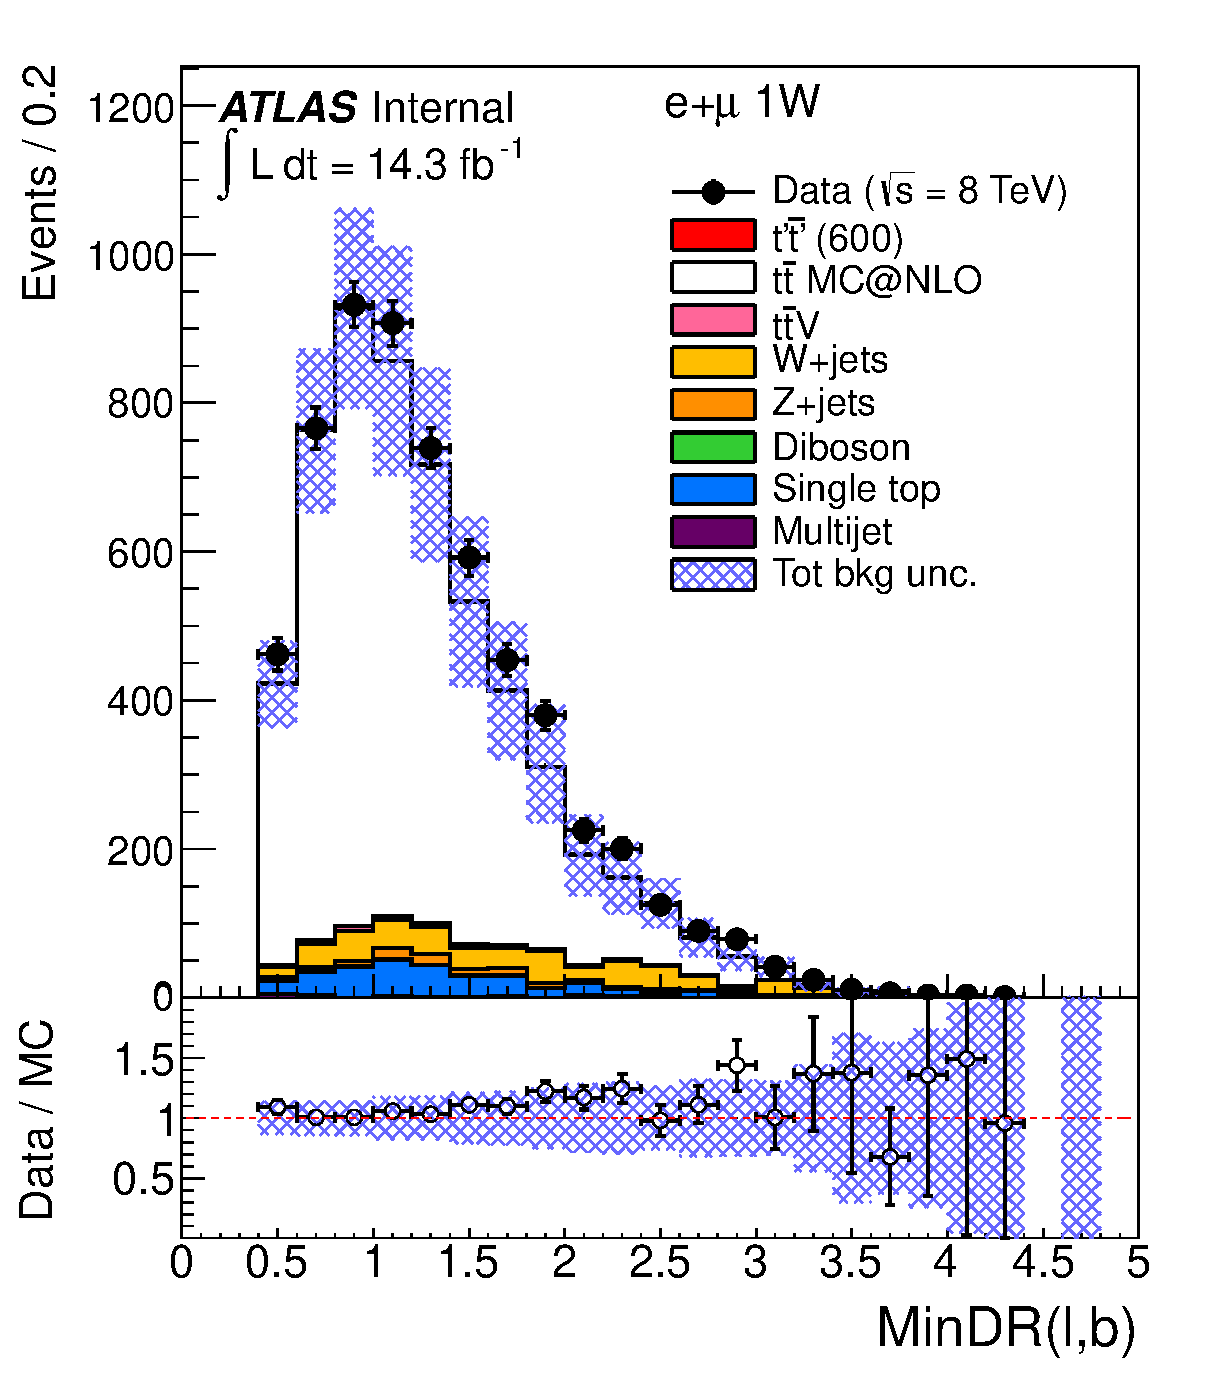
\includegraphics[width=0.30\textwidth]{appendices/figures/sdrs/VLQAna_WbX_MinDRlb_ELEMUONCR0_1W_NOMINAL.eps} \\
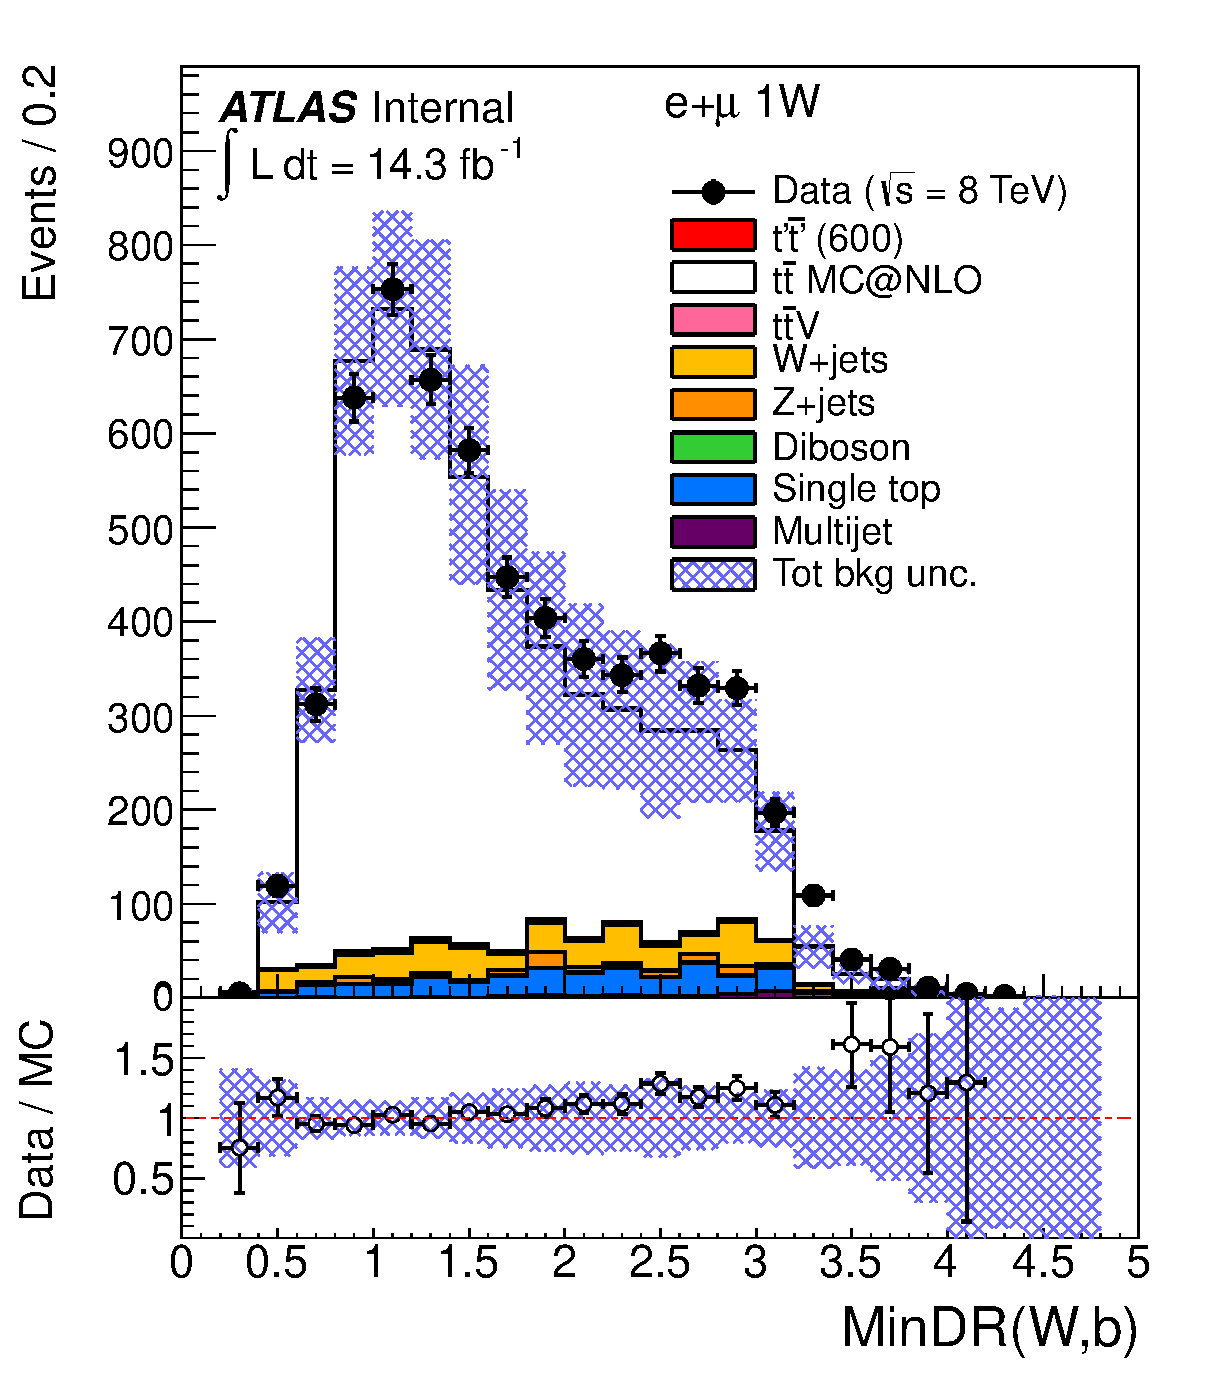
\includegraphics[width=0.30\textwidth]{appendices/figures/sdrs/VLQAna_WbX_MinDRWb_ELEMUONCR0_1W_NOMINAL.eps} &
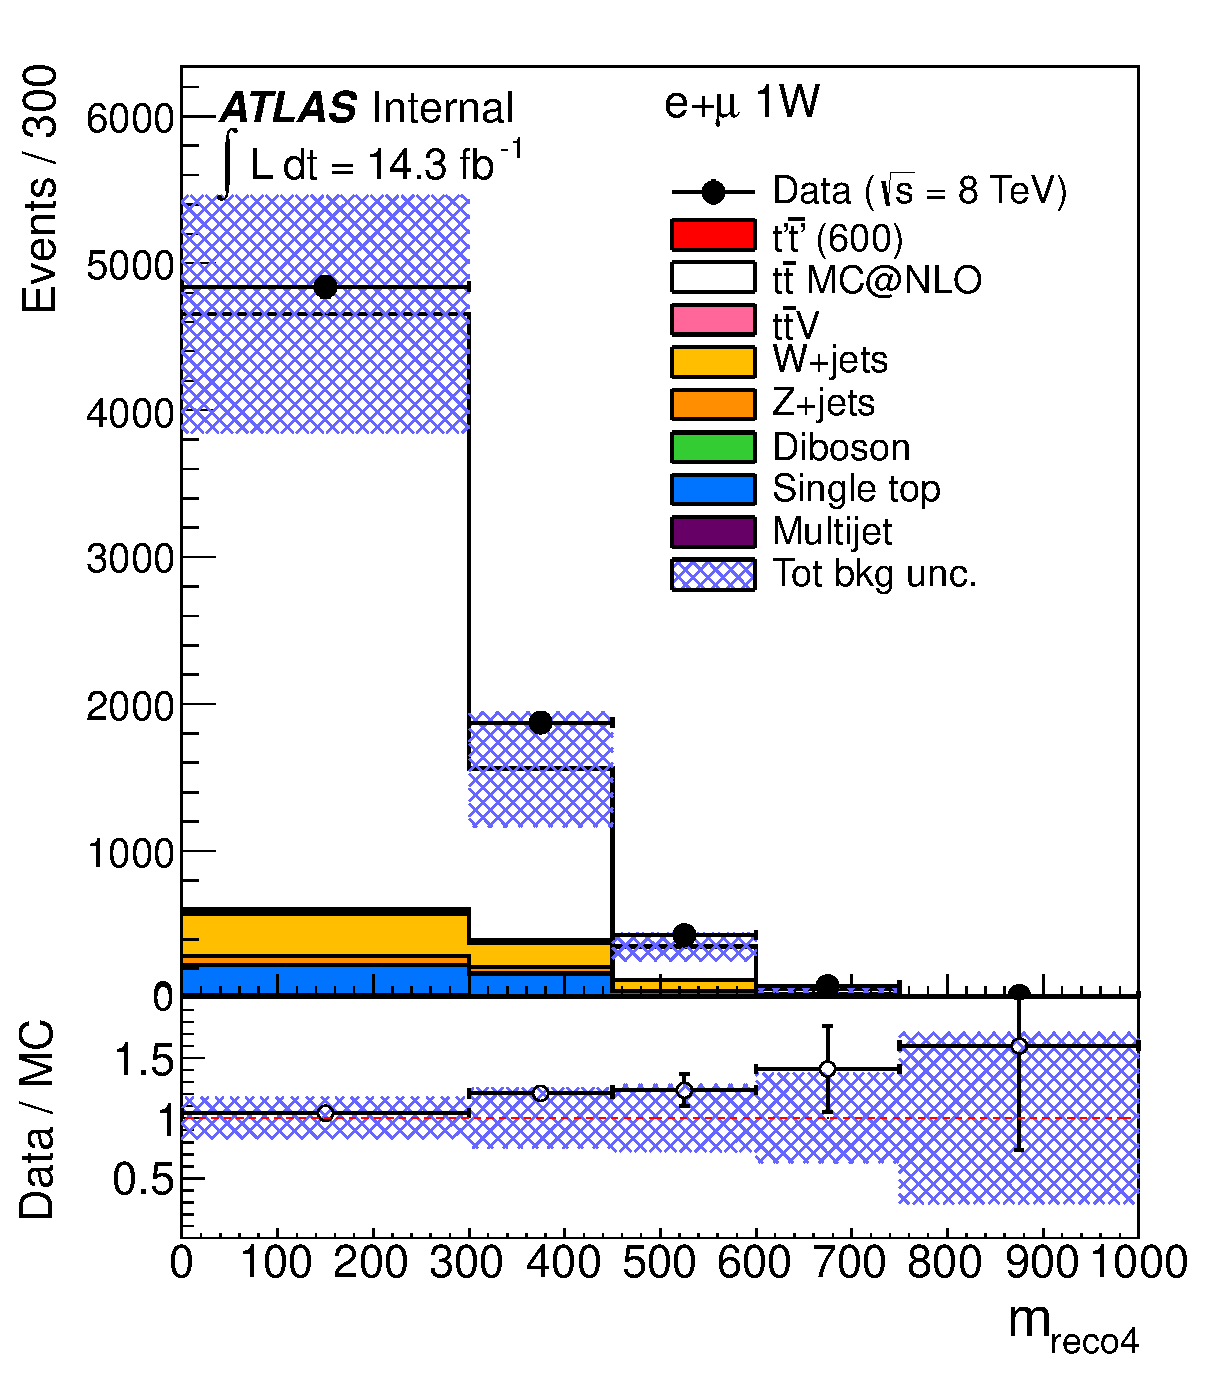
\includegraphics[width=0.30\textwidth]{appendices/figures/sdrs/VLQAna_WbX_1W_MWb_4_ELEMUONCR0_1W_NOMINAL.eps} & \\
\end{tabular}\caption{\small {Comparison between data and prediction in combined $e$+jets and $\mu$+jets channel in SDR0 (see Sect.~\ref{sec:sdrs} for details) 
for a number of kinematic variables. From top to bottom and left to right, the variables displayed are: $\pt$ for leading and second-leading $b$ jets,
number of $W_{\rm had}$  candidates, $\pt$ of selected $W_{\rm had}$  candidate, $\Delta R(\ell,\nu)$, $\min(\Delta R(\ell, b_{1,2}))$, 
$\min(\Delta R(W_{\rm had}, b_{1,2}))$ and $m_{\rm reco}$.
The shaded area represents the total background uncertainty.}}
\label{fig:ELEMUONCR0_3}
\end{center}
\end{figure}                                                                             
%%%%%%%%%%%%%%

\begin{landscape}
\begin{figure}[htb]\begin{center}
\vskip-1.5cm
\hskip-2cm
\resizebox{1.5\textwidth}{!}{
	\subfigure[]{
          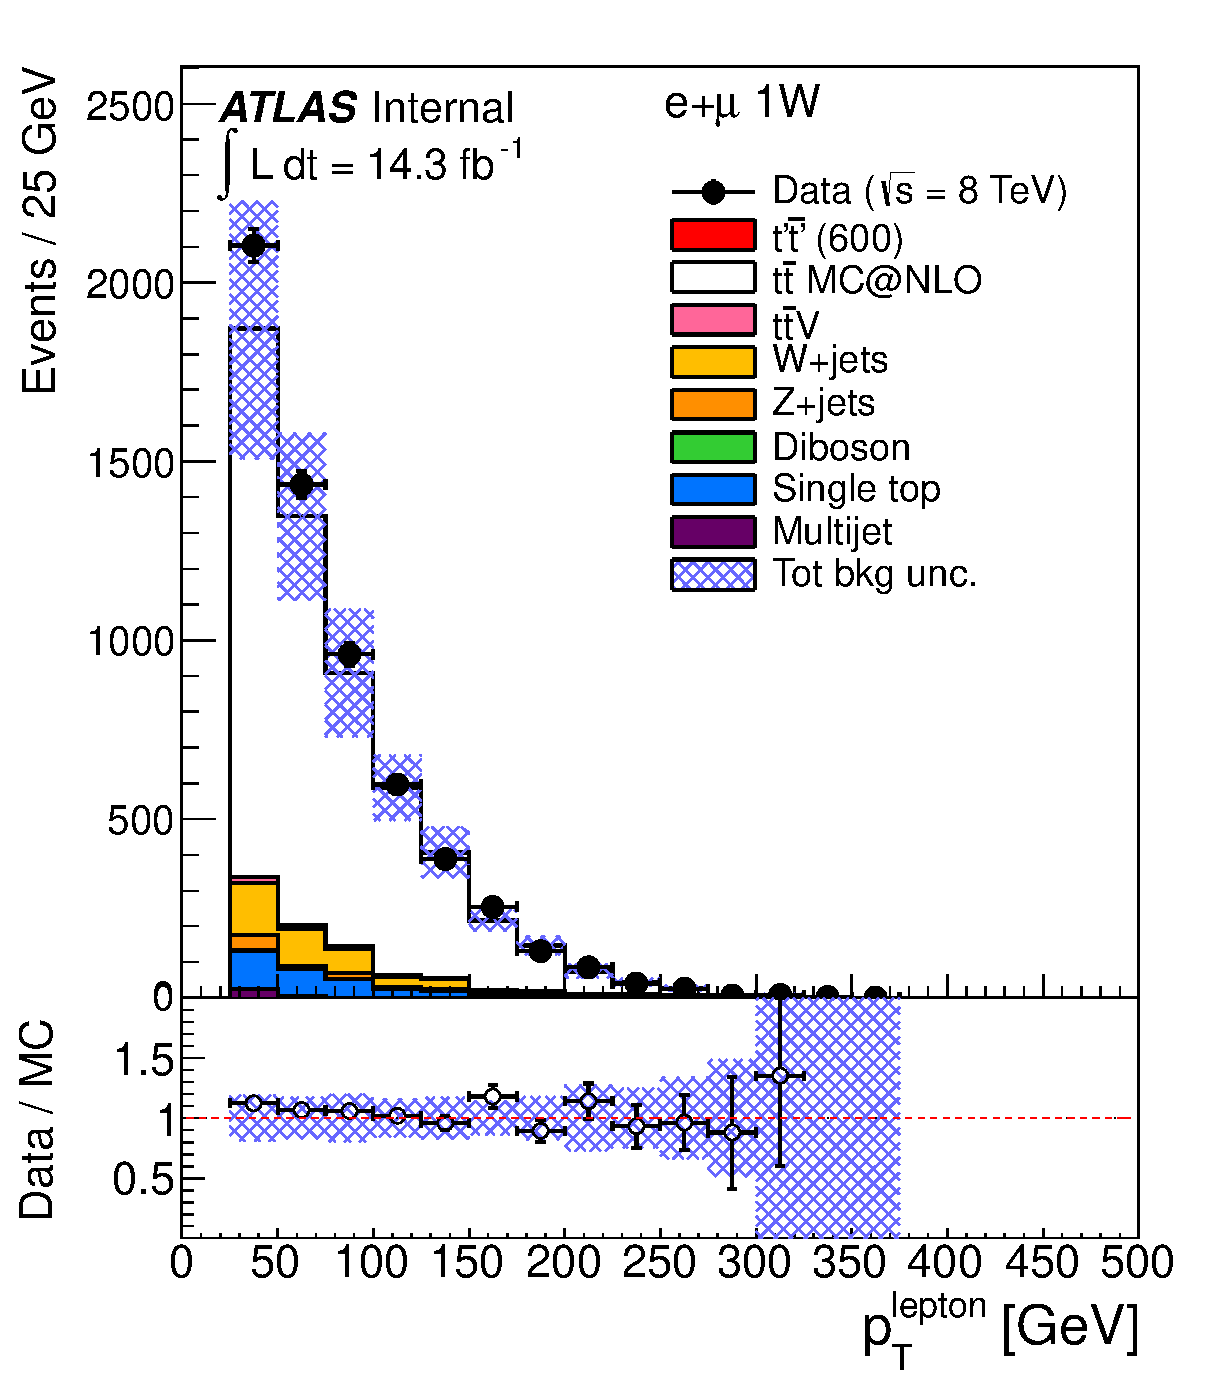
\includegraphics[width=0.3\textwidth]{appendices/figures/sdrs/LepPt_ELEMUONCR0_1W_NOMINAL.eps}}
	\subfigure[]{
          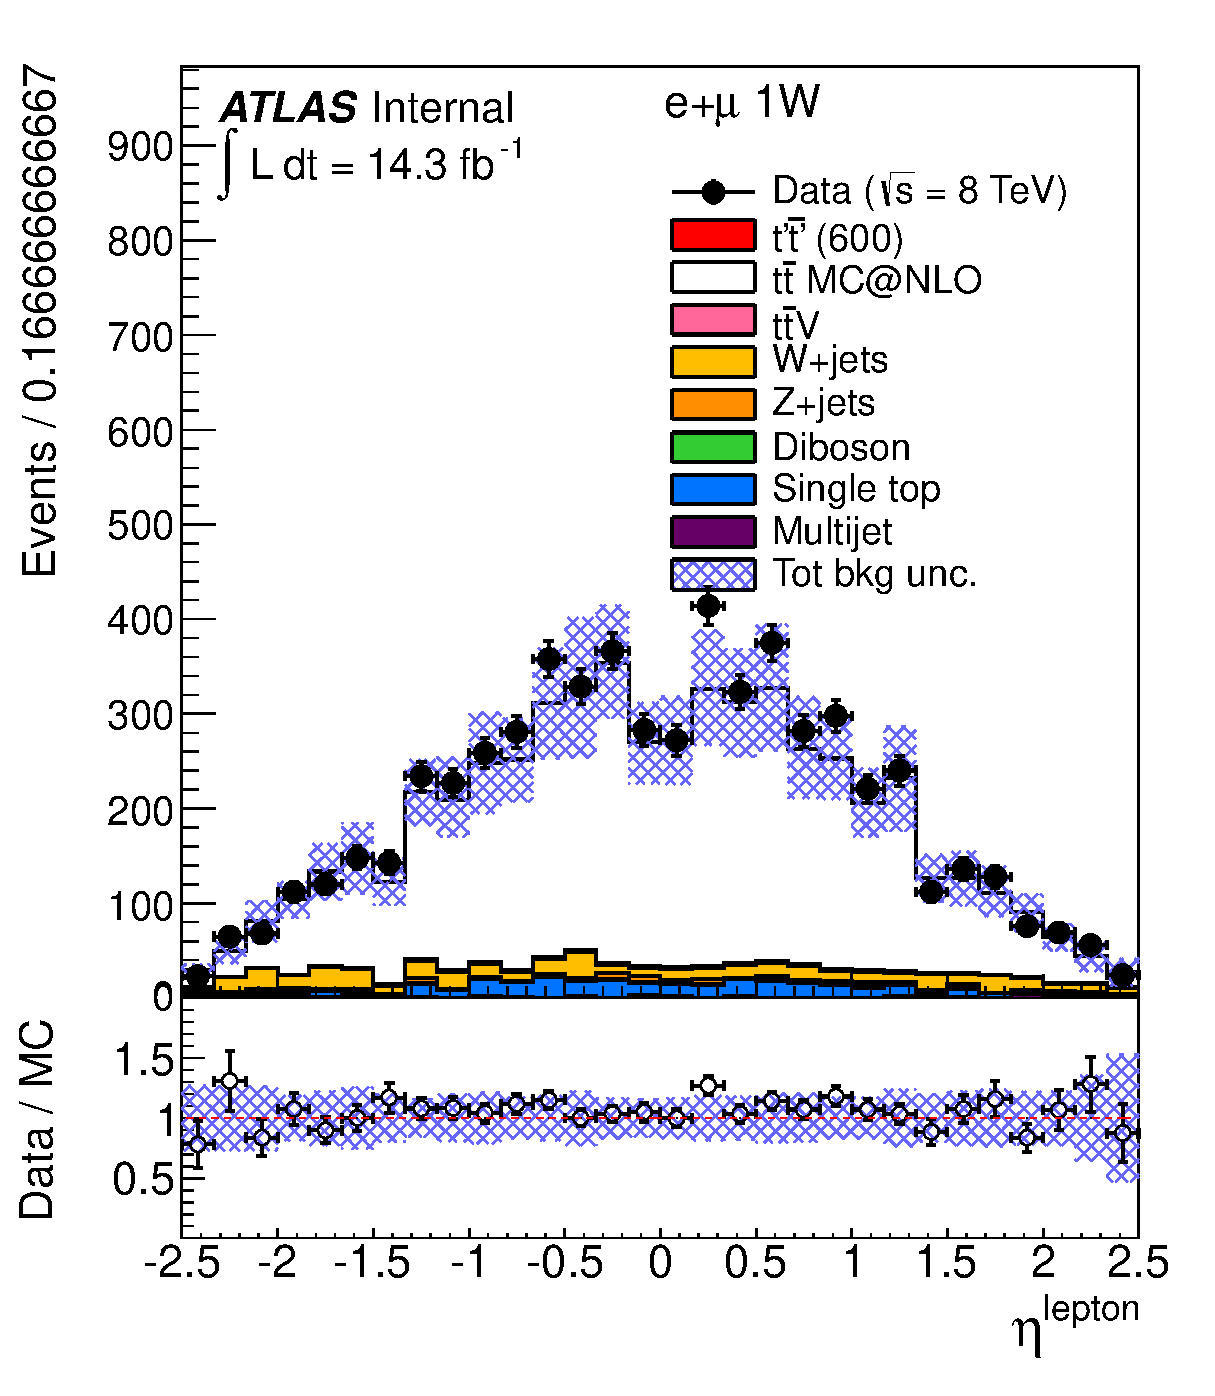
\includegraphics[width=0.3\textwidth]{appendices/figures/sdrs/LepEta_ELEMUONCR0_1W_NOMINAL.eps}}
	\subfigure[]{
          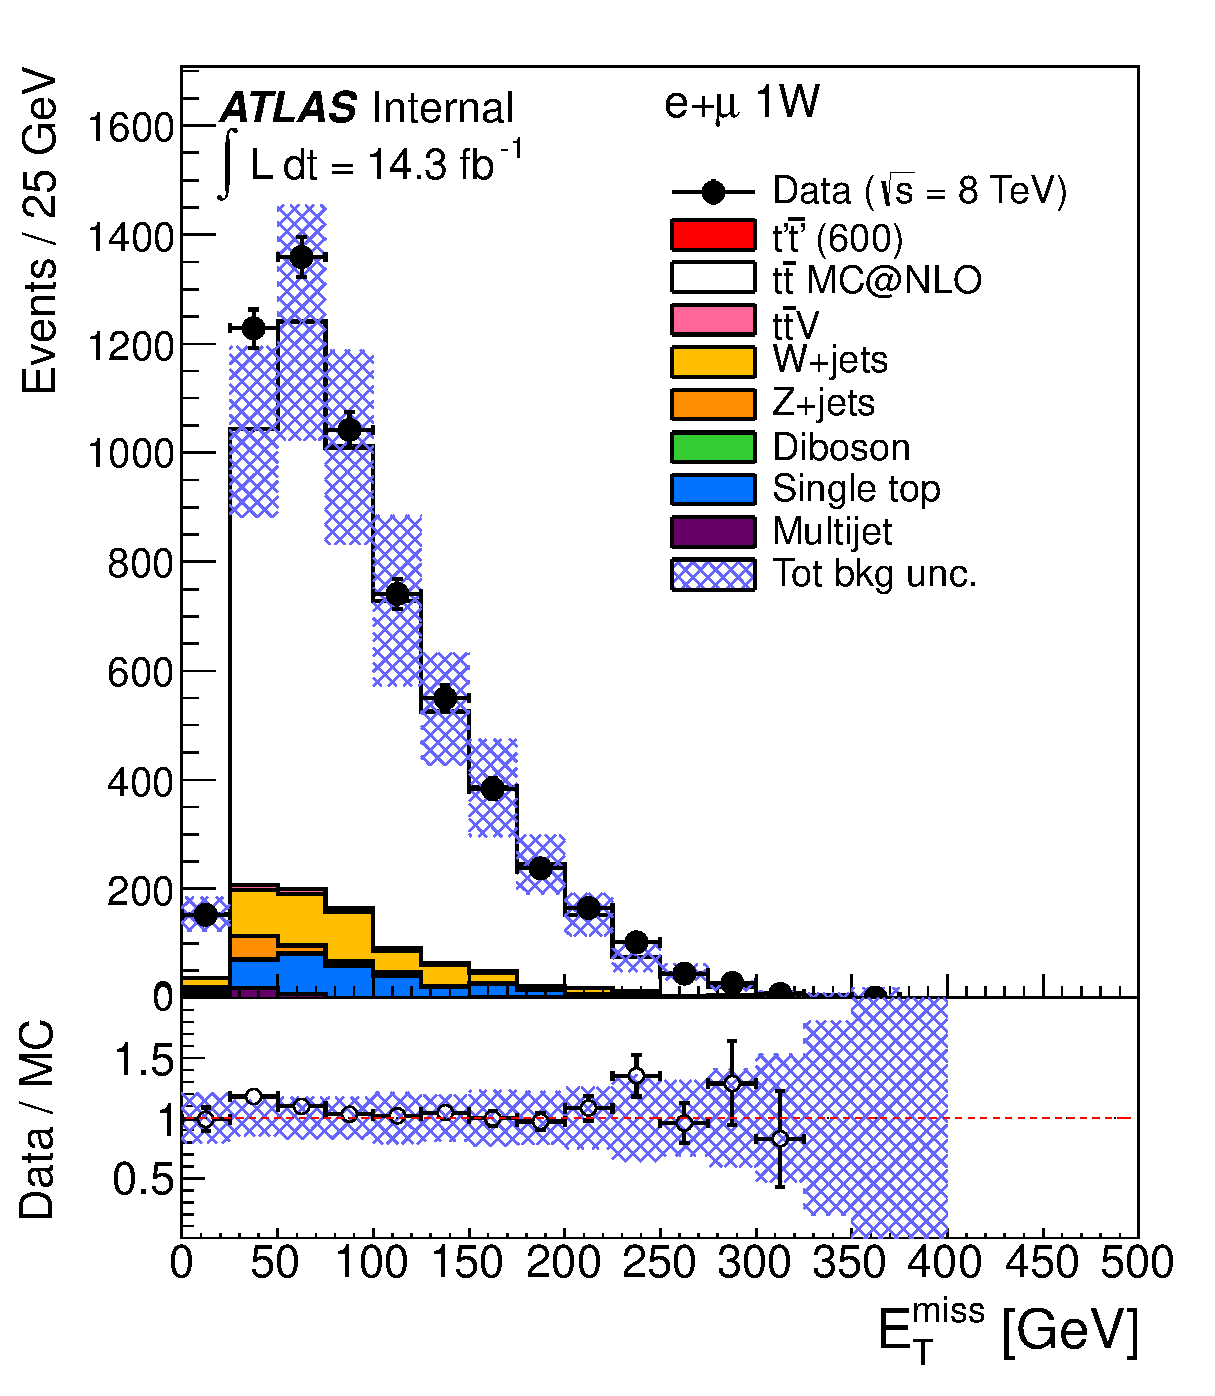
\includegraphics[width=0.3\textwidth]{appendices/figures/sdrs/MET_ELEMUONCR0_1W_NOMINAL.eps}}
	\subfigure[]{
          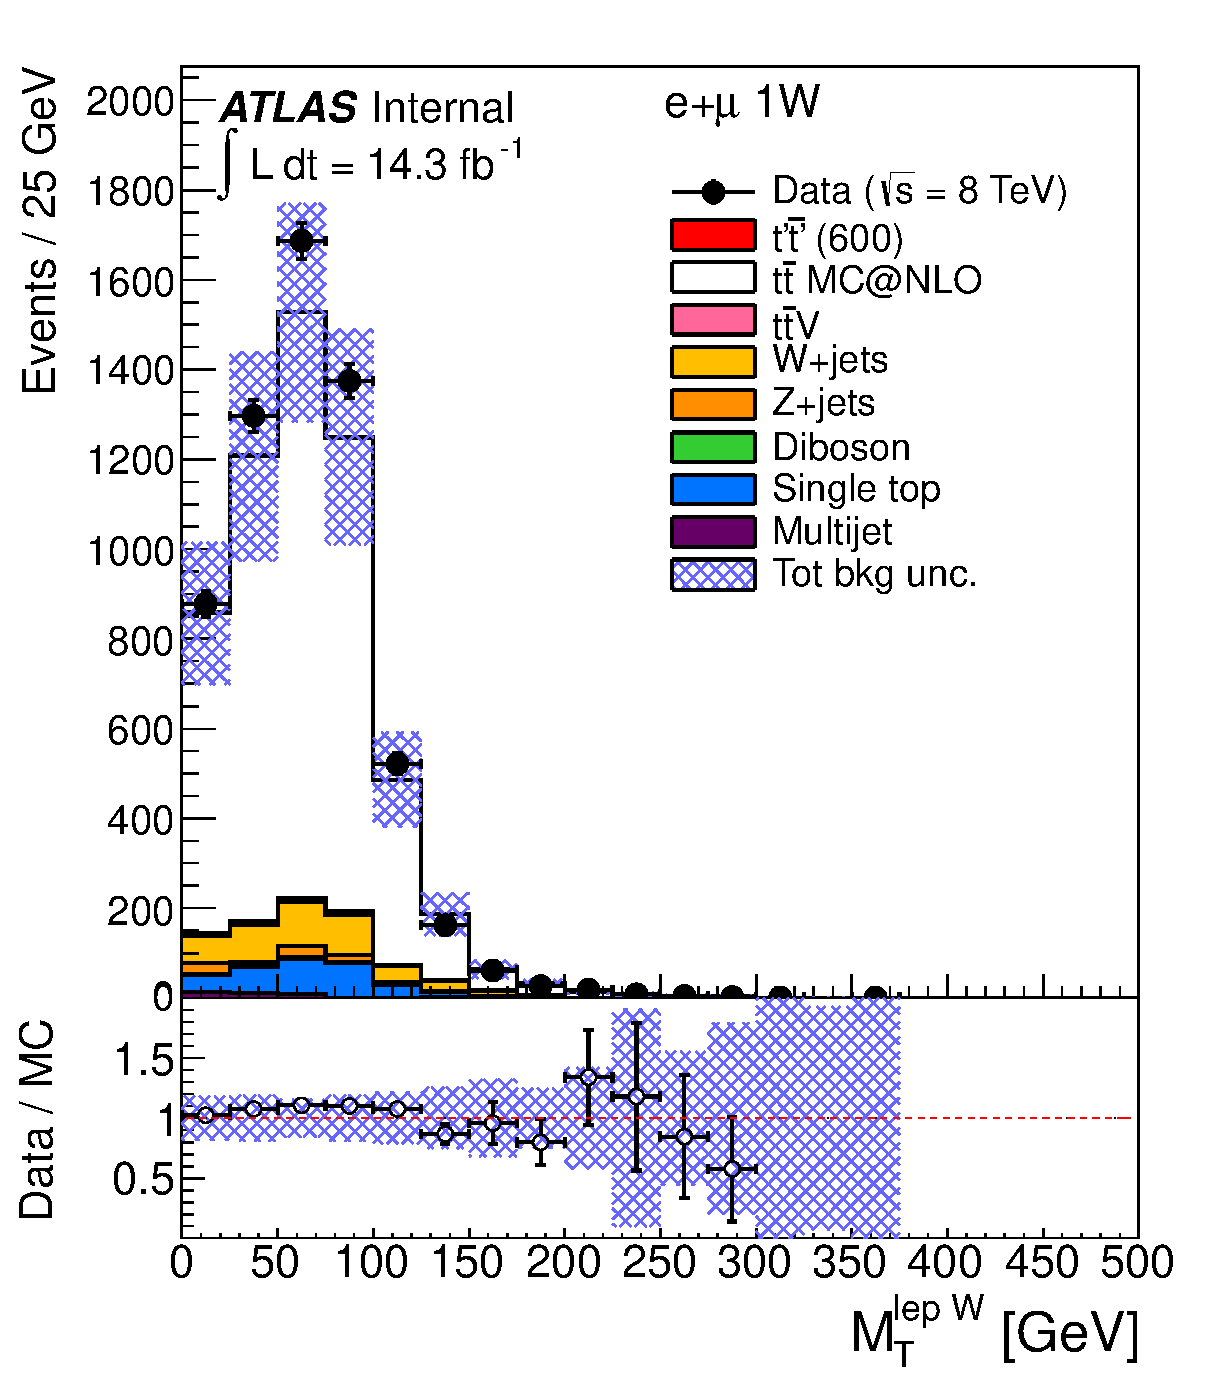
\includegraphics[width=0.3\textwidth]{appendices/figures/sdrs/Wlep_MassT_ELEMUONCR0_1W_NOMINAL.eps}}
	\subfigure[]{
          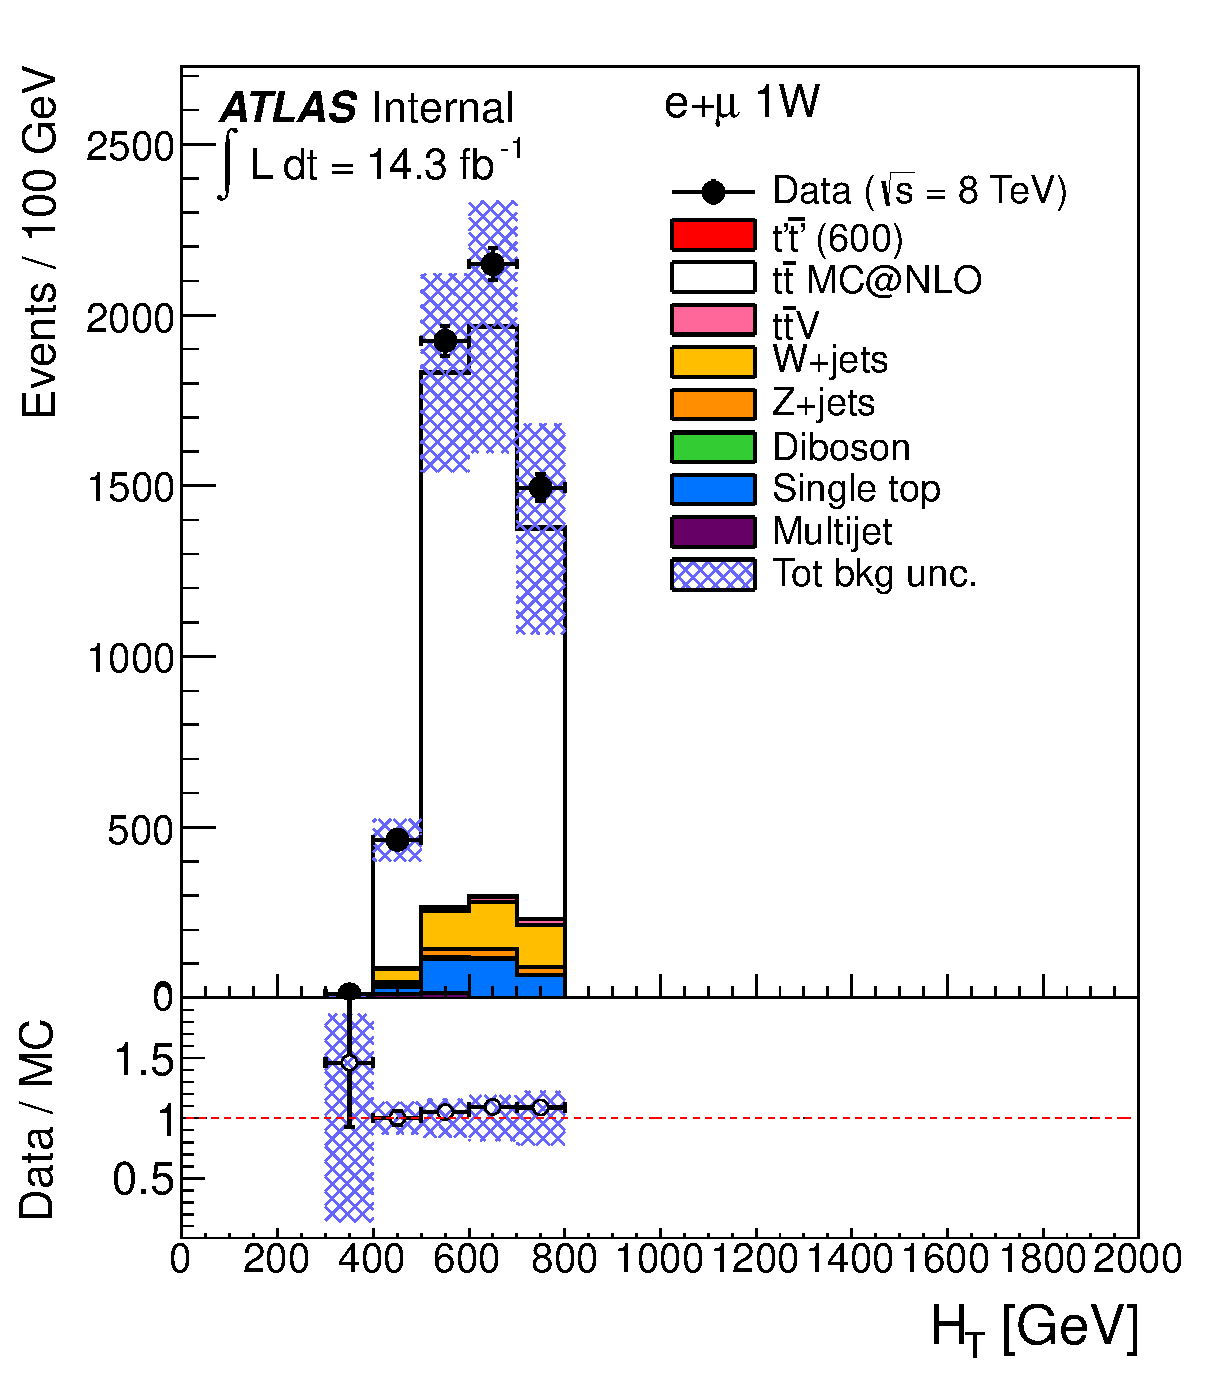
\includegraphics[width=0.3\textwidth]{appendices/figures/sdrs/HTAll_ELEMUONCR0_1W_NOMINAL.eps}}
}\\
\hskip-2cm
\resizebox{1.5\textwidth}{!}{
	\subfigure[]{
          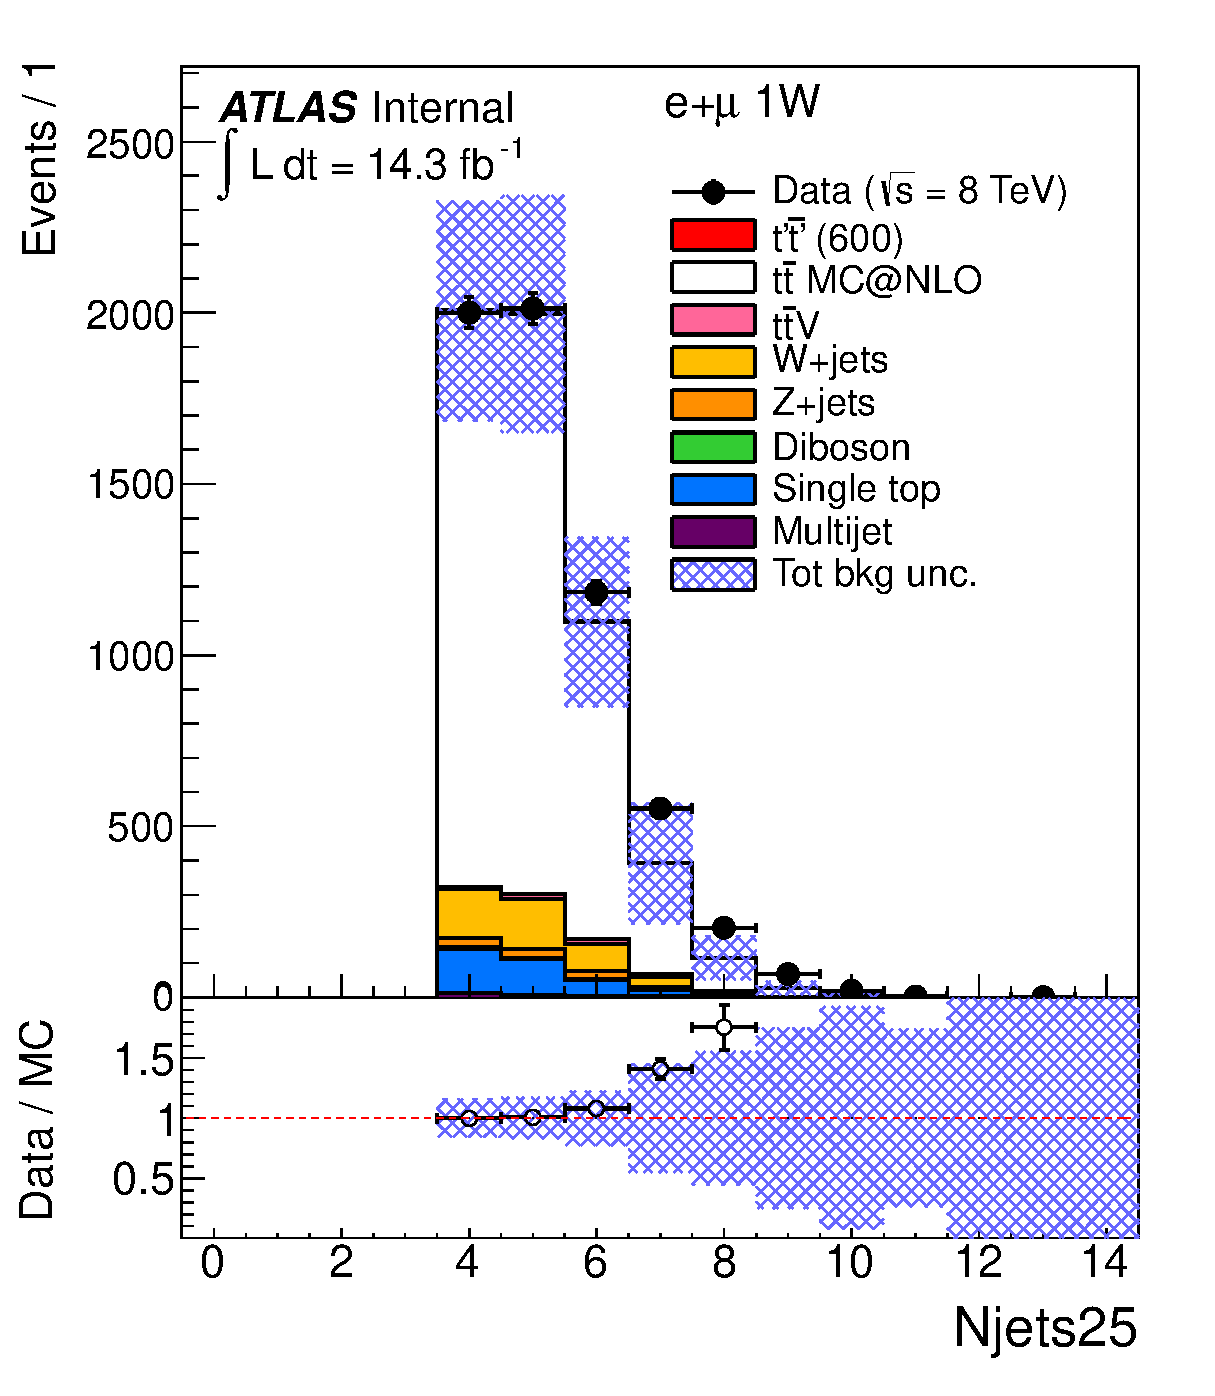
\includegraphics[width=0.3\textwidth]{appendices/figures/sdrs/Njets25_ELEMUONCR0_1W_NOMINAL.eps}}
	\subfigure[]{
          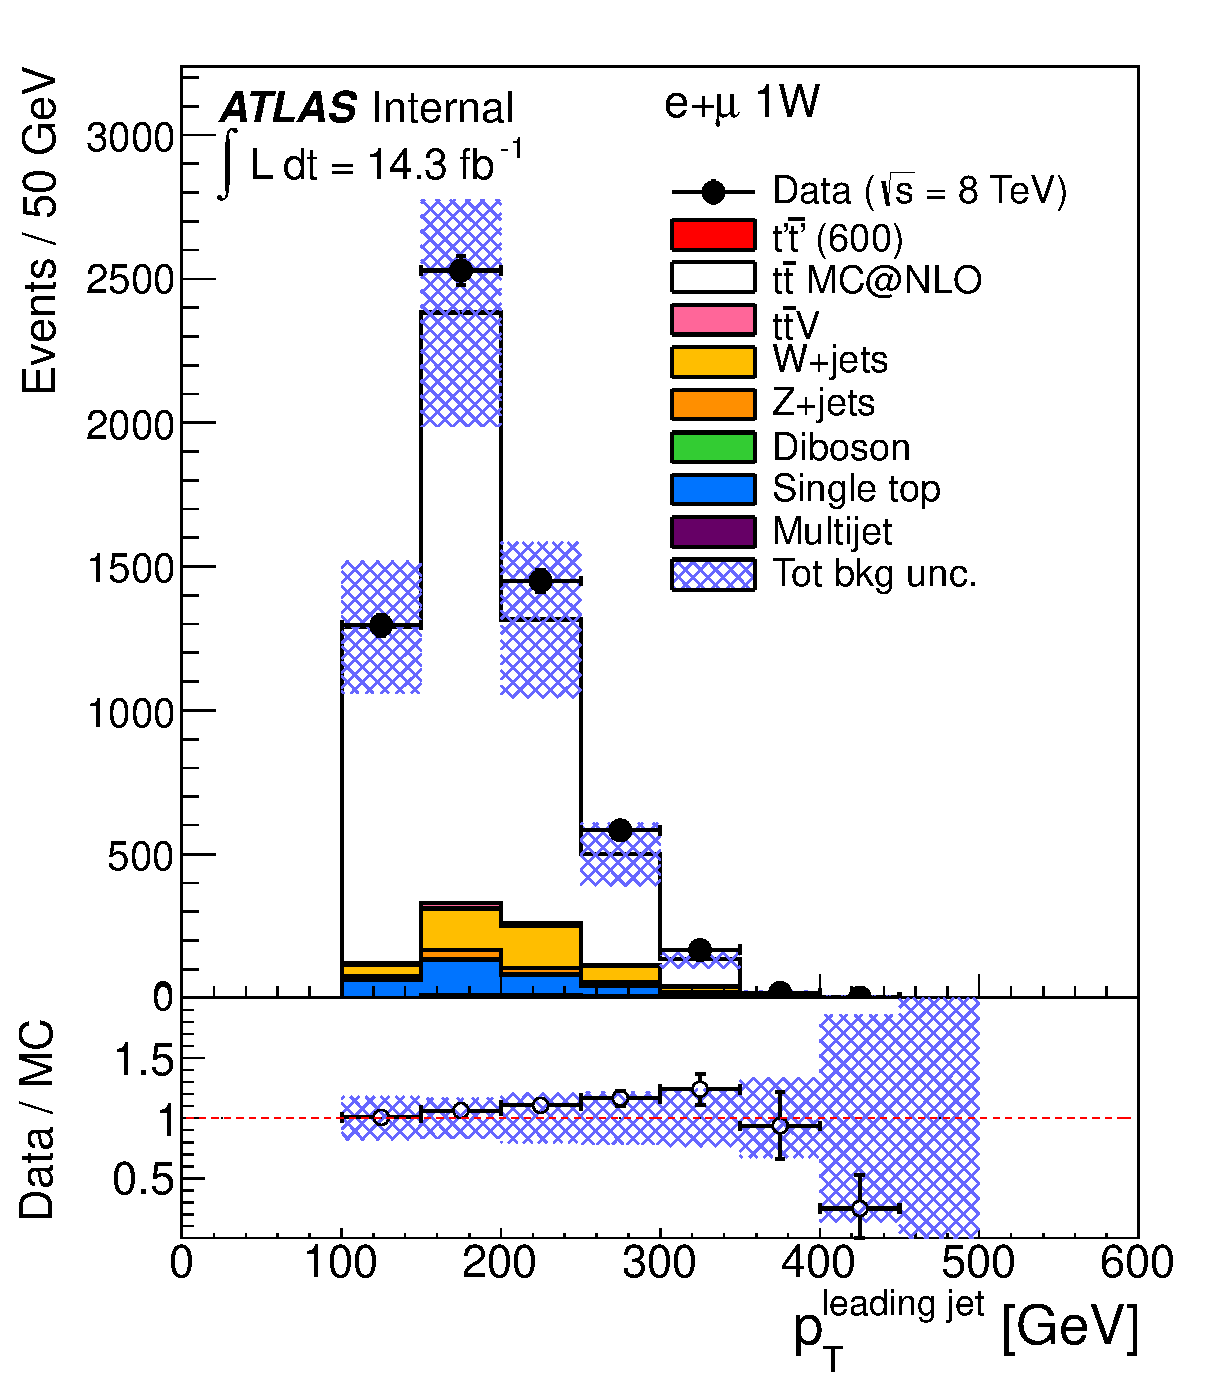
\includegraphics[width=0.3\textwidth]{appendices/figures/sdrs/JetPt1_ELEMUONCR0_1W_NOMINAL.eps}}
	\subfigure[]{
          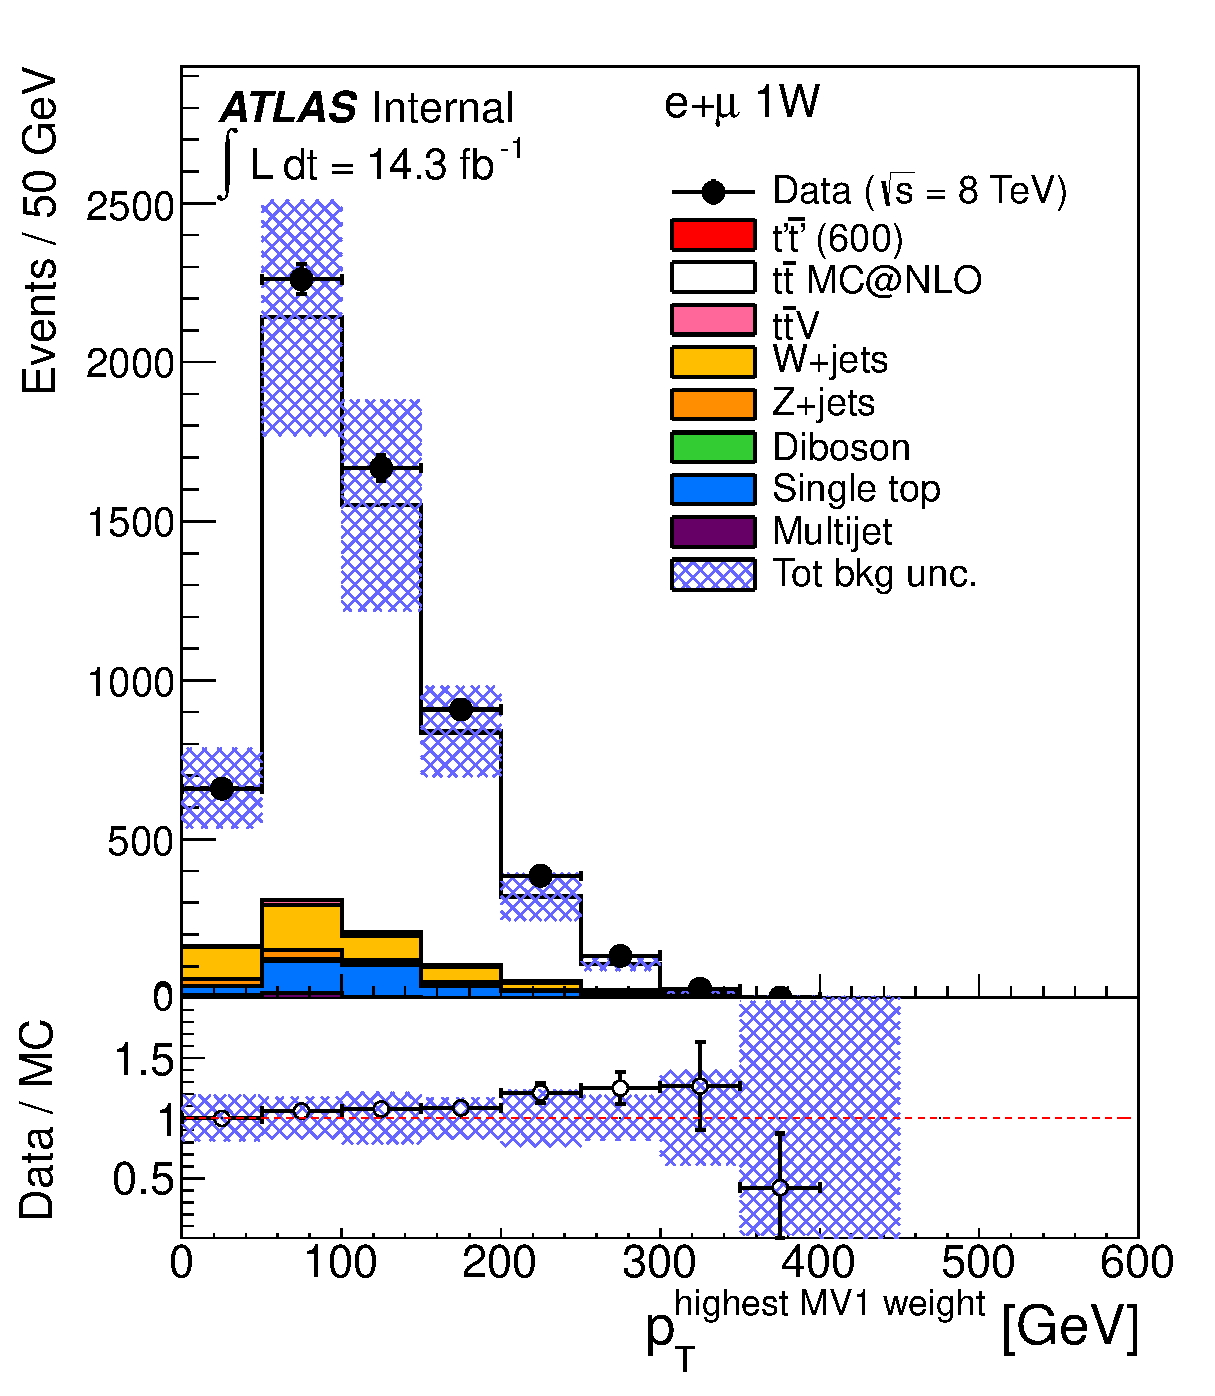
\includegraphics[width=0.3\textwidth]{appendices/figures/sdrs/JetPtB1_ELEMUONCR0_1W_NOMINAL.eps}}
	\subfigure[]{
          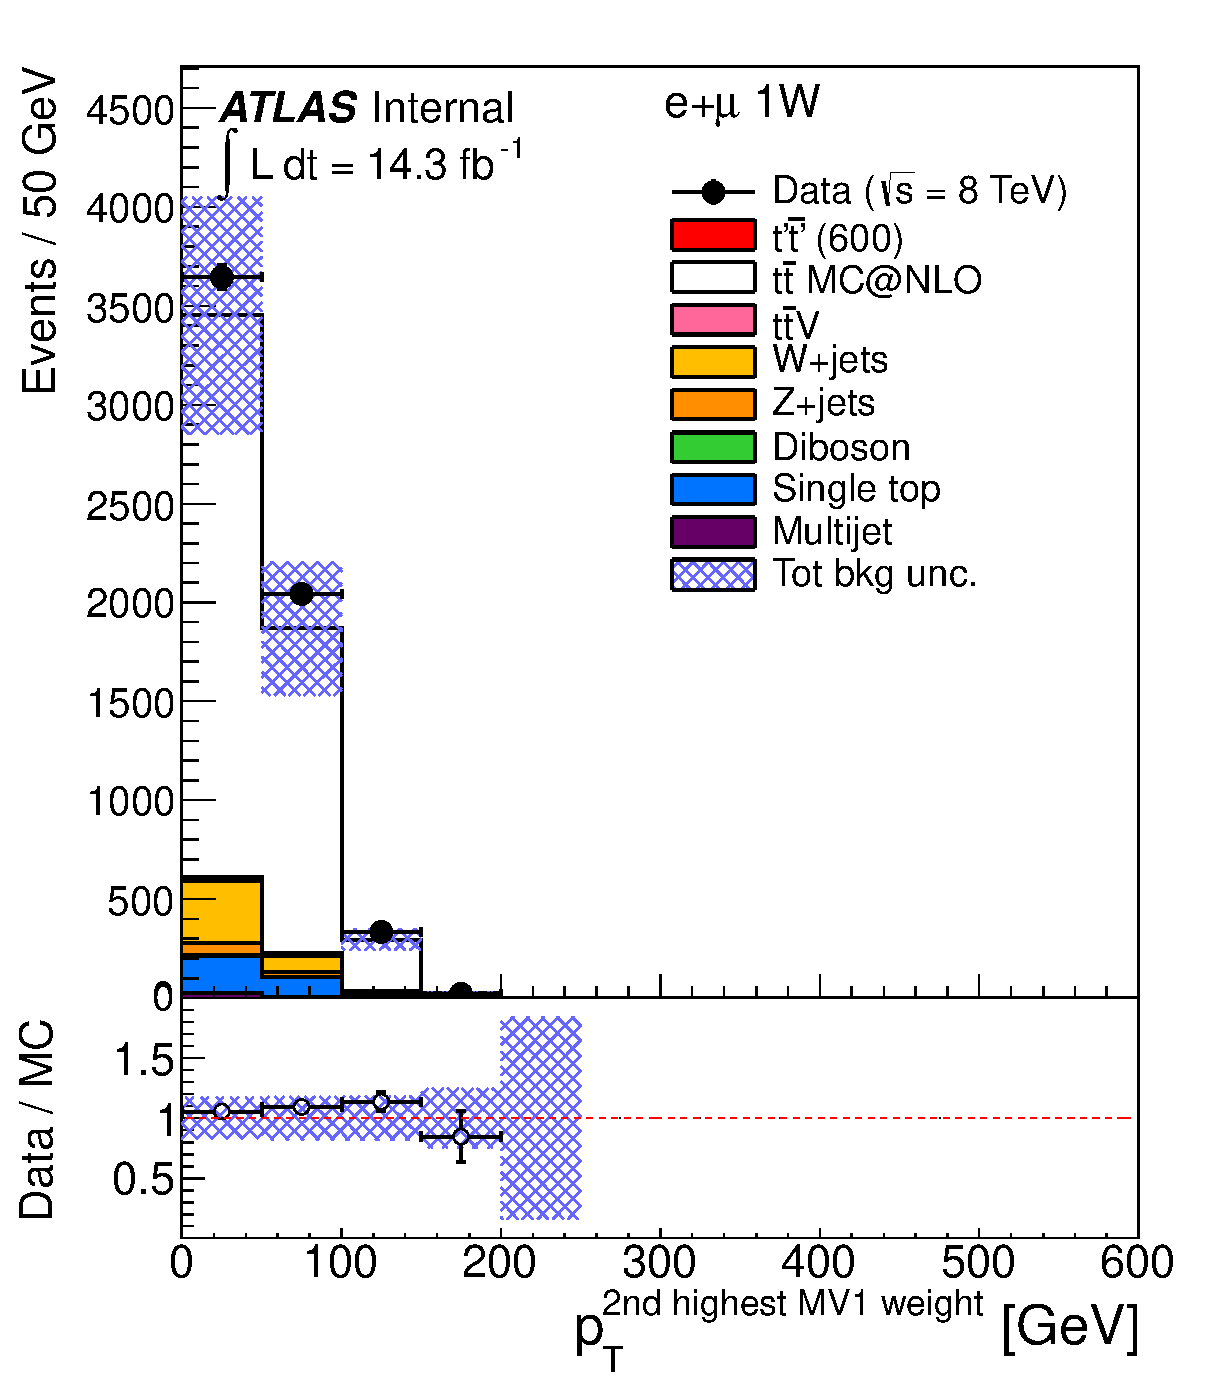
\includegraphics[width=0.3\textwidth]{appendices/figures/sdrs/JetPtB2_ELEMUONCR0_1W_NOMINAL.eps}}
	\subfigure[]{
          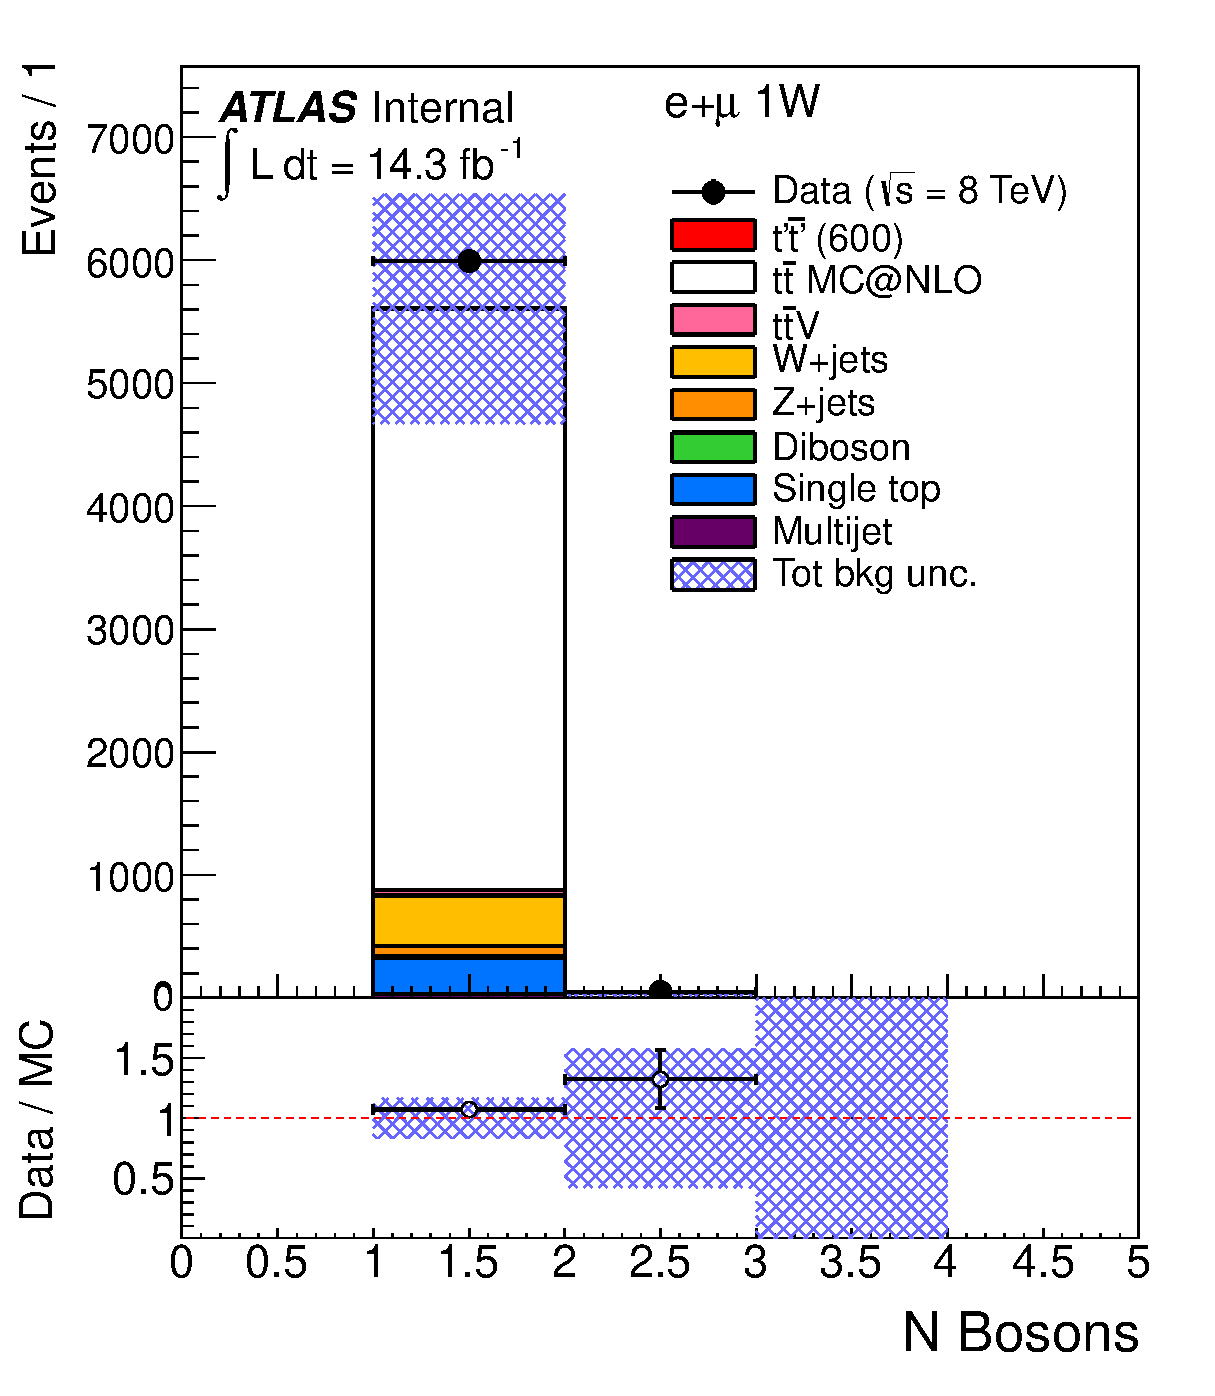
\includegraphics[width=0.3\textwidth]{appendices/figures/sdrs/nWhad_ELEMUONCR0_1W_NOMINAL.eps}}
}\\
\hskip-2cm
\resizebox{1.5\textwidth}{!}{
	\subfigure[]{
          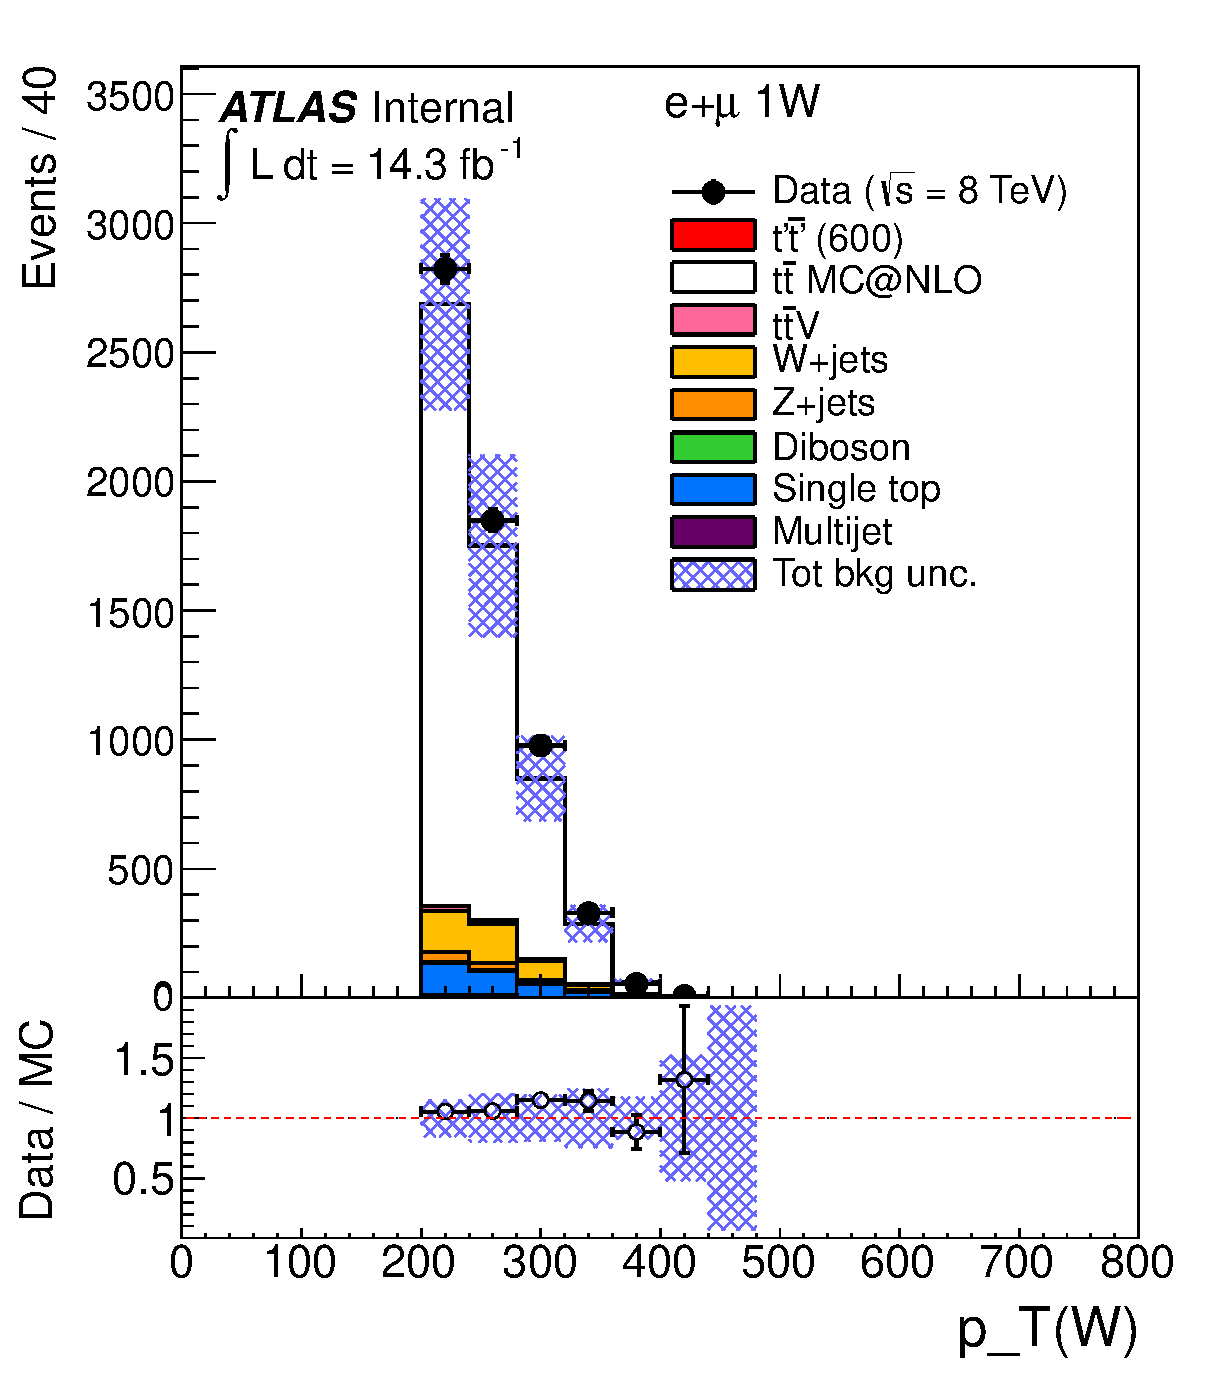
\includegraphics[width=0.3\textwidth]{appendices/figures/sdrs/VLQAna_WbX_W1Pt_ELEMUONCR0_1W_NOMINAL.eps}}
	\subfigure[]{
          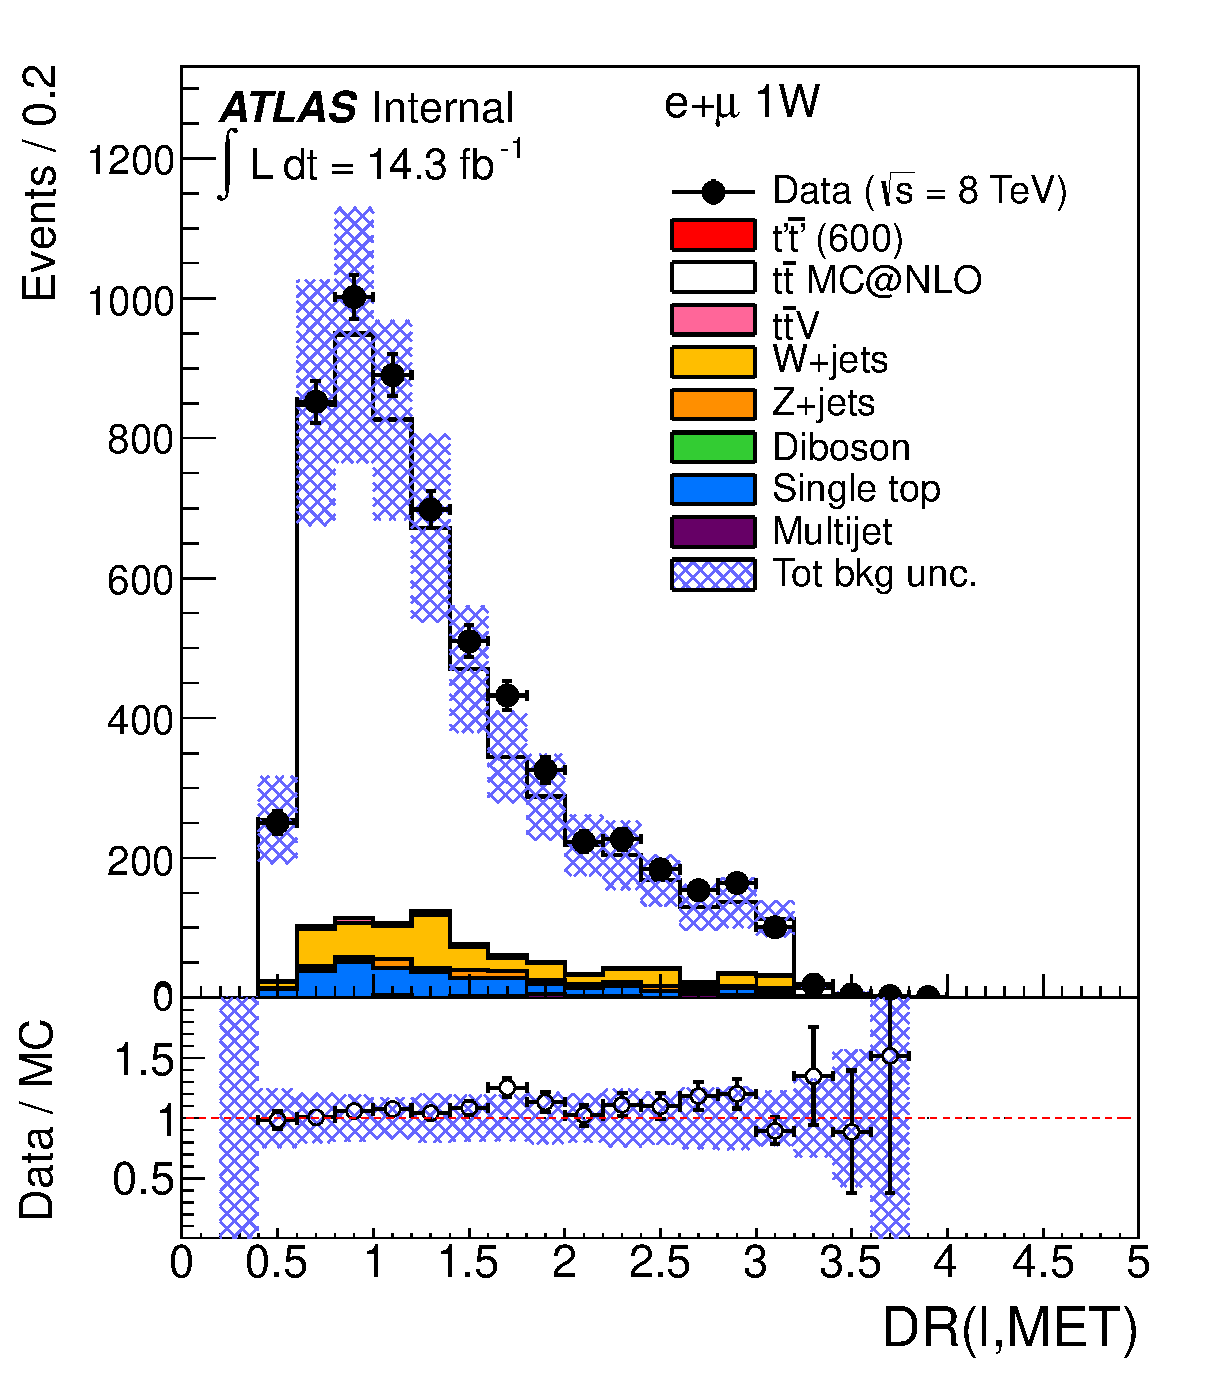
\includegraphics[width=0.3\textwidth]{appendices/figures/sdrs/VLQAna_WbX_DRLepMet_ELEMUONCR0_1W_NOMINAL.eps}}
	\subfigure[]{
          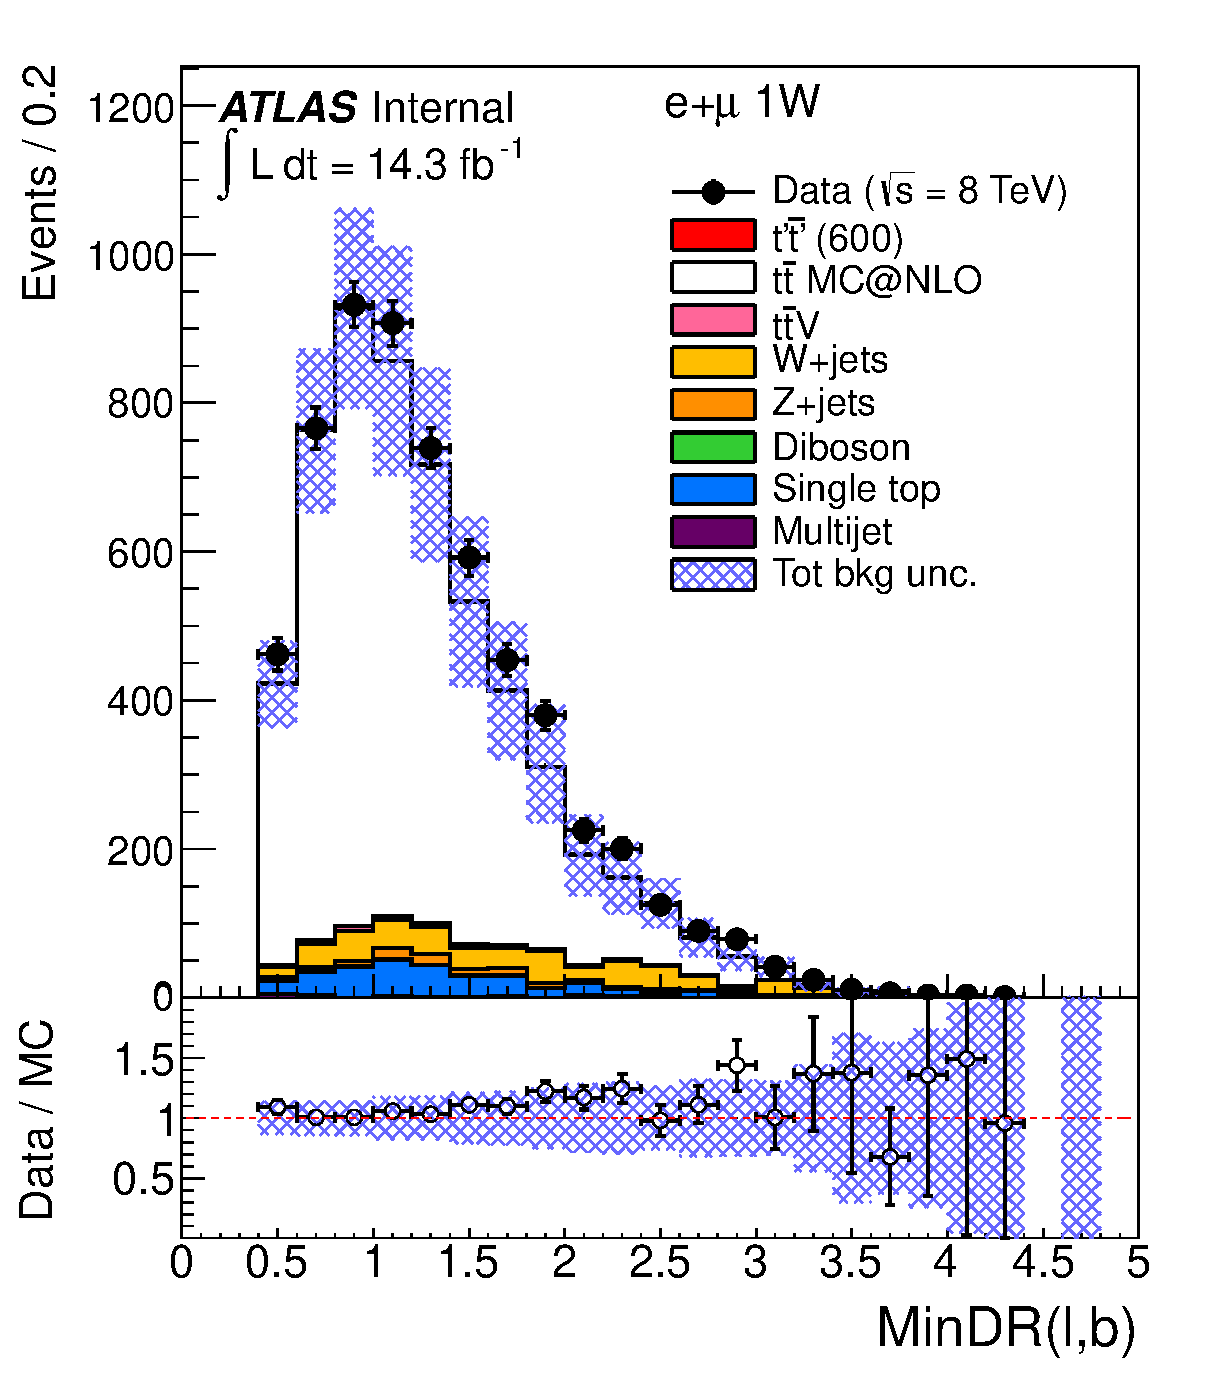
\includegraphics[width=0.3\textwidth]{appendices/figures/sdrs/VLQAna_WbX_MinDRlb_ELEMUONCR0_1W_NOMINAL.eps}}
	\subfigure[]{
          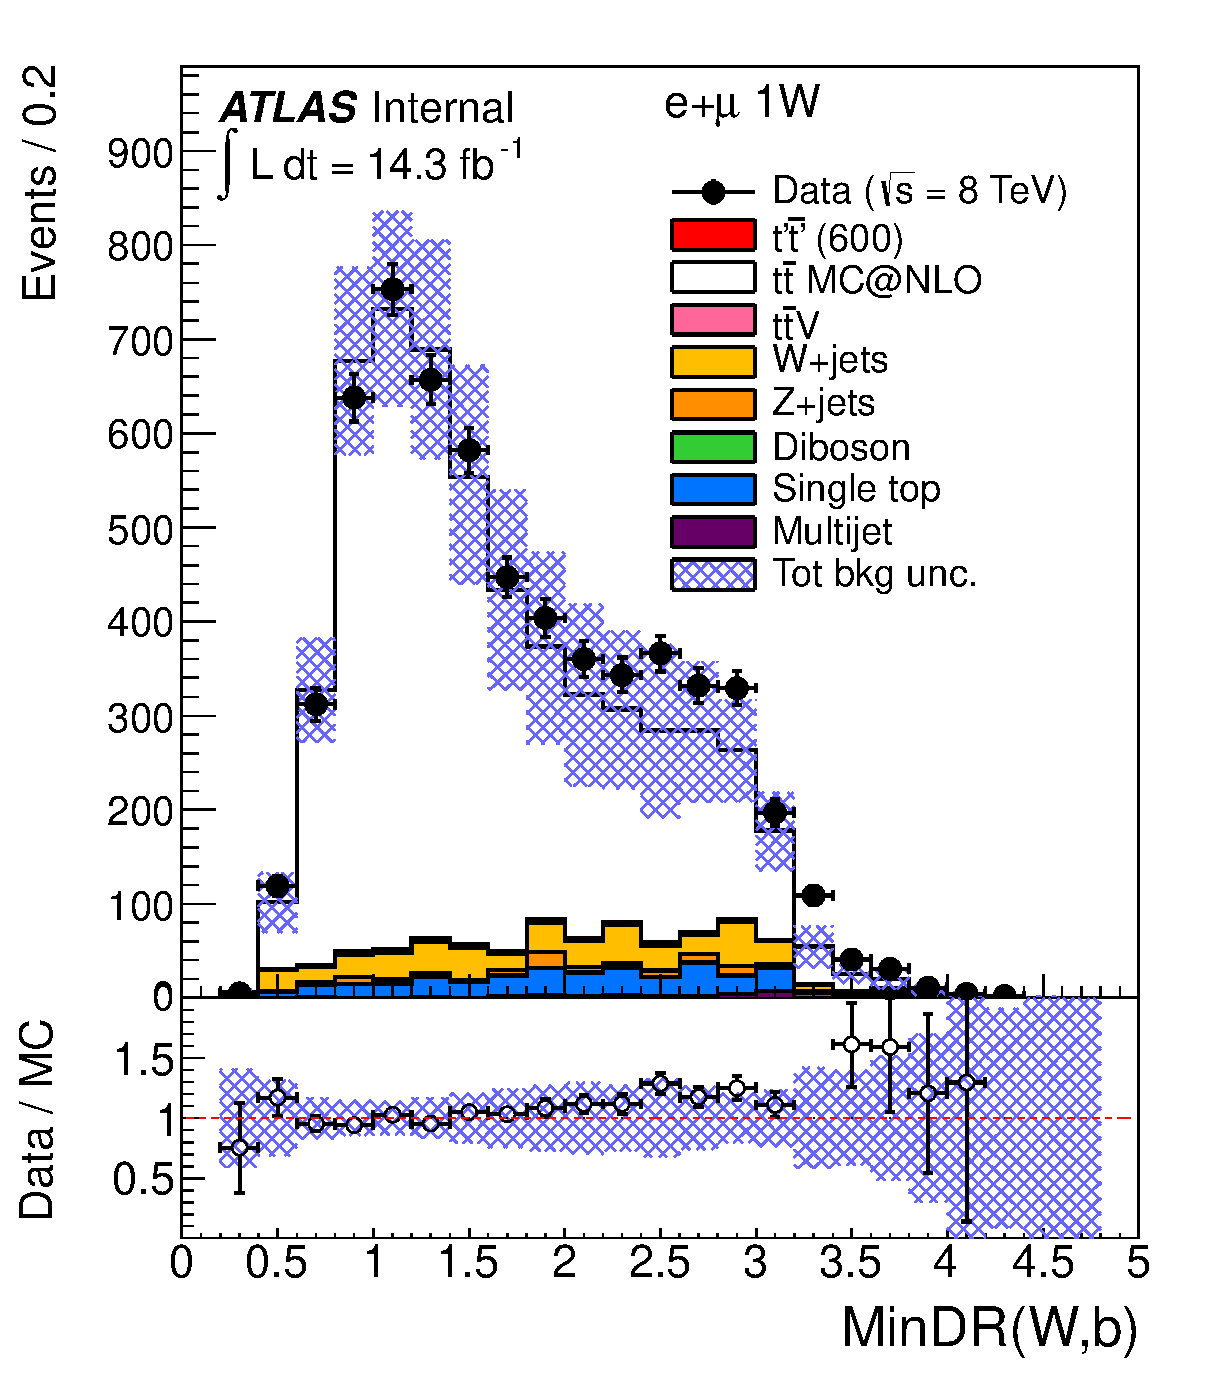
\includegraphics[width=0.3\textwidth]{appendices/figures/sdrs/VLQAna_WbX_MinDRWb_ELEMUONCR0_1W_NOMINAL.eps}}
	\subfigure[]{
          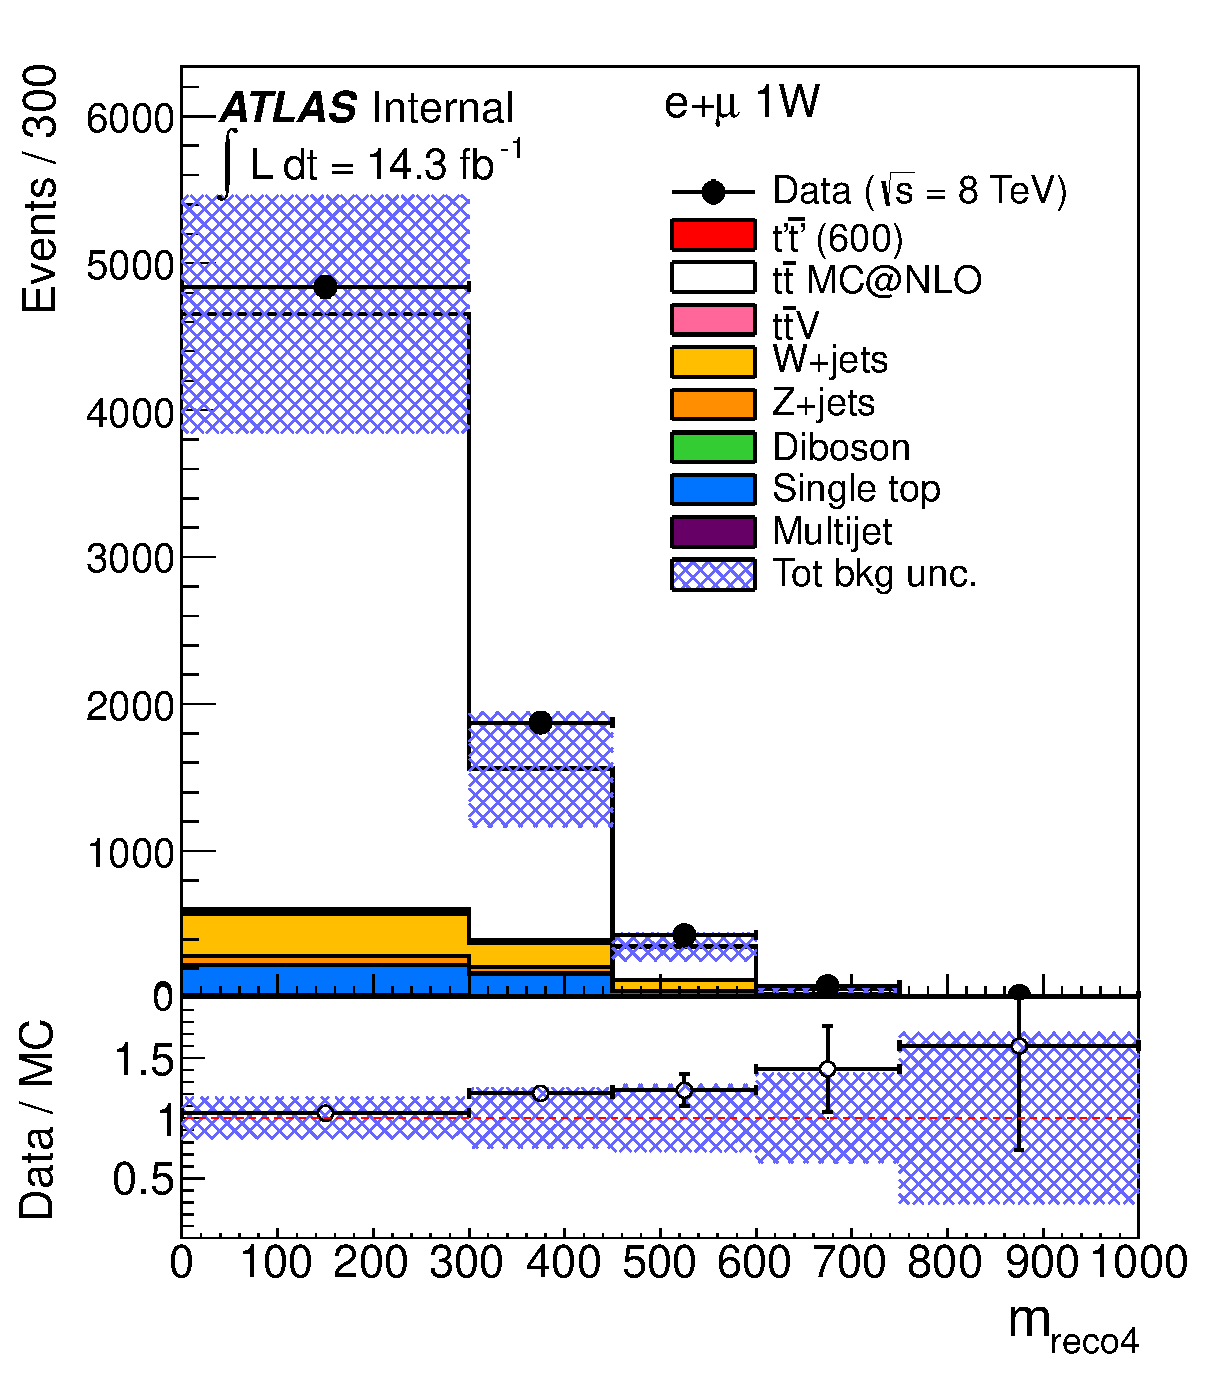
\includegraphics[width=0.3\textwidth]{appendices/figures/sdrs/VLQAna_WbX_1W_MWb_4_ELEMUONCR0_1W_NOMINAL.eps}}
}
	\caption{Comparison between data and prediction in combined $e$+jets and $\mu$+jets combined channel in SDR0
          for a number of kinematic variables: 
          %%%row 1
          (a)  lepton $\pt$, (b) lepton $\eta$, (c) missing transverse energy, 
          (d)  $W$ transverse mass, (e) $\HT$ variable, 
          %%%row 2
          (f) number of jets with $\pt>25\gev$, (g) leading jet $\pt$, 
          (h) $\pt$ for leading \bjet, (i) $\pt$ for second-leading \bjet,
          (j) number of $W_{\rm had}$  candidates, 
          %%%row 3
          (k) $\pt$ of selected $W_{\rm had}$  candidate, 
          (l) $\Delta R(\ell,\nu)$, (m) $\min(\Delta R(\ell, b_{1,2}))$, 
          (n) $\min(\Delta R(W_{\rm had}, b_{1,2}))$ and (o) $m_{\rm reco}$.
          The shaded area represents the total background uncertainty.\label{fig:ELEMUONCR0}}
\end{center}\end{figure}
\end{landscape}


\clearpage

\section{Comparison between data and prediction in SDR1}
\label{sec:DataMC_CR5}

SDR1: preselection cuts, $\geq 1$ $W_{\rm had}$ candidates, $m_{\rm reco}<200\gev$. The $m_{\rm reco}$ variable represents the
reconstructed heavy quark mass and is defined in Section~\ref{sec:wbxDISCR}. 

%%%%%%%%%%%%%%%
\begin{table}[h!]
\begin{center}
\renewcommand{\arraystretch}{1.3}
\begin{tabular}{l*{1}{r@{ $\pm$ }r@{ }l}}
\hline\hline
 & \multicolumn{3}{c}{ELEMUONCR5\_1W}\\
\hline
$T\bar{T}(600\GeV)$ (Chiral) & $7.07$ & $0.94$ & $^{+2.91}_{-2.19}$\\
\hline
$t\bar{t}$ & $3870.01$ & $38.16$ & $^{+612.74}_{-702.94}$\\
$W$+jets & $218.14$ & $21.80$ & $^{+92.42}_{-85.97}$\\
$Z$+jets & $41.06$ & $7.35$ & $^{+20.80}_{-25.36}$\\
Diboson & $1.88$ & $0.35$ & $^{+0.77}_{-0.74}$\\
Single top & $136.68$ & $7.11$ & $^{+22.98}_{-18.41}$\\
$t\bar{t}$$V$ & $30.24$ & $0.44$ & $^{+9.28}_{-9.32}$\\
Multijet & $-2.84$ & $23.67$ & $ \pm\ 0.00$\\
\hline
Total bkg. & $4295.16 $ & $ 50.96$ & $ ^{+679.61}_{-773.95}$\\
\hline
Data & \multicolumn{3}{c}{$4174$}\\
\hline\hline
\end{tabular}

\vspace{0.5cm}

\caption{\small{Number of observed events compared to the SM expectation for
the combined electron and muon channels in SDR1 (see Section~\ref{sec:wbxCR} for details) . 
The expected signal yield assuming $m_{\T}=600\gev$ for the chiral scenario is also shown. 
The quoted uncertainties include both statistical and systematic contributions.}}
\label{tab:CR5_1W_evtable}
\end{center}
\end{table}
%%%%%%%%%%%%%%%

\clearpage

%%%%%%%%%%%%%%%
\begin{figure}[h!]
\begin{center}
\begin{tabular}{ccc}
%
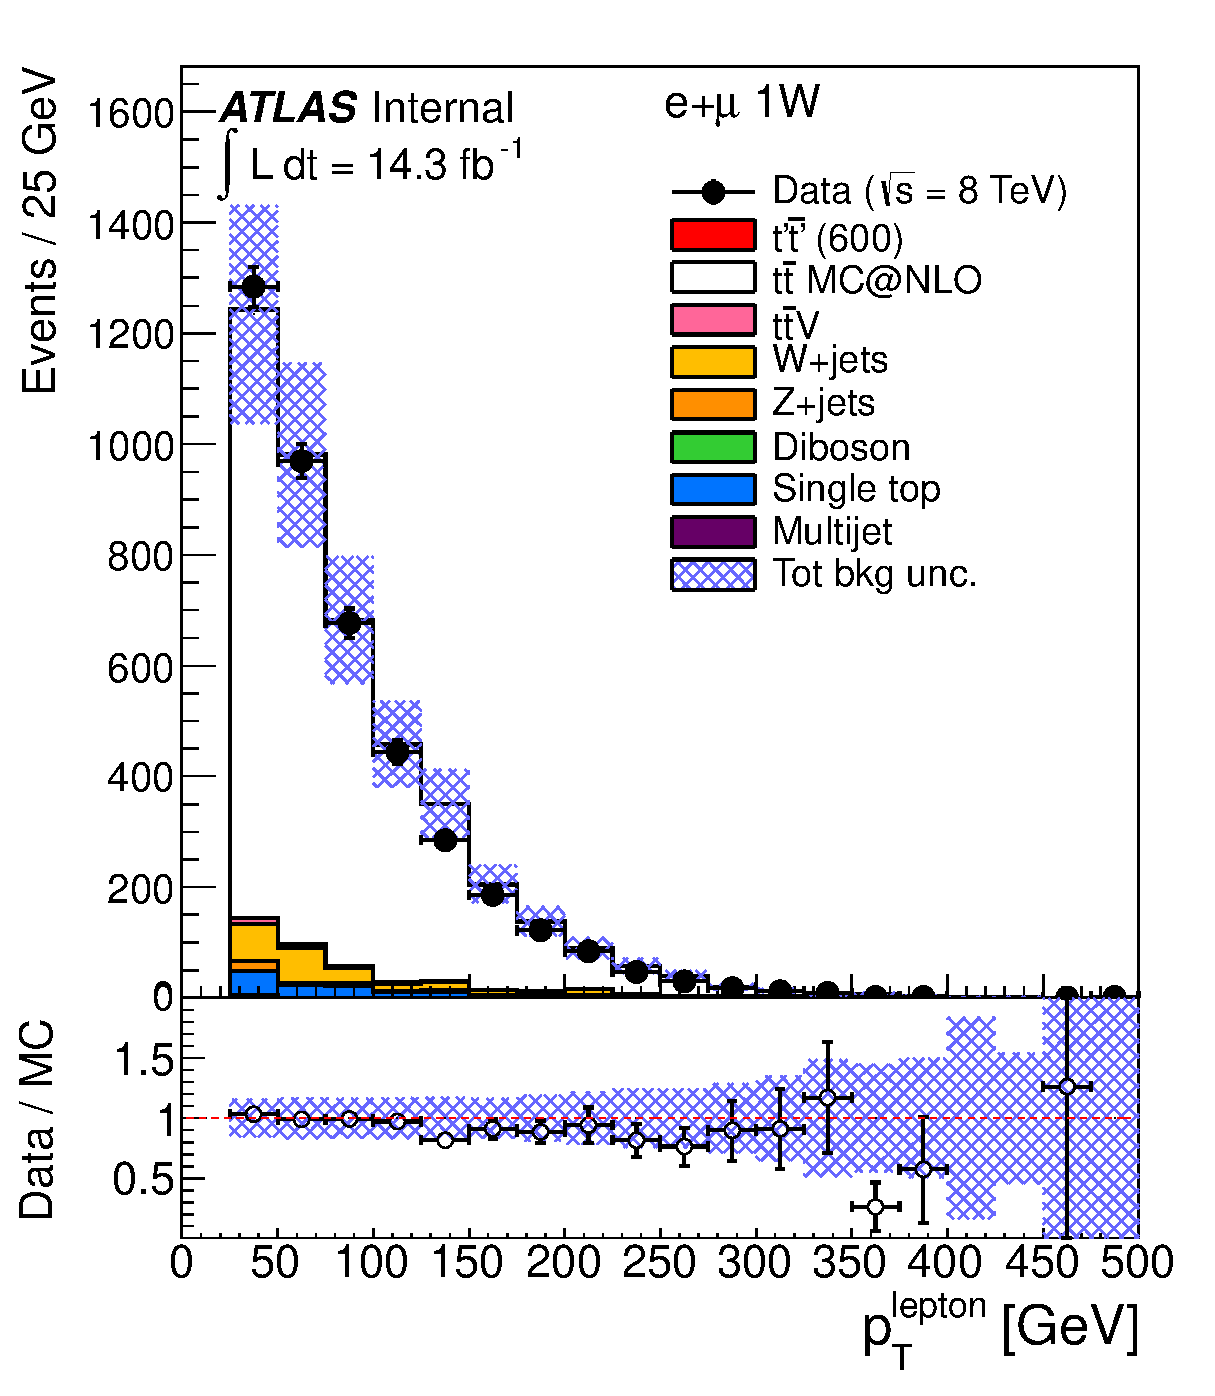
\includegraphics[width=0.30\textwidth]{appendices/figures/sdrs/LepPt_ELEMUONCR5_1W_NOMINAL.eps} &
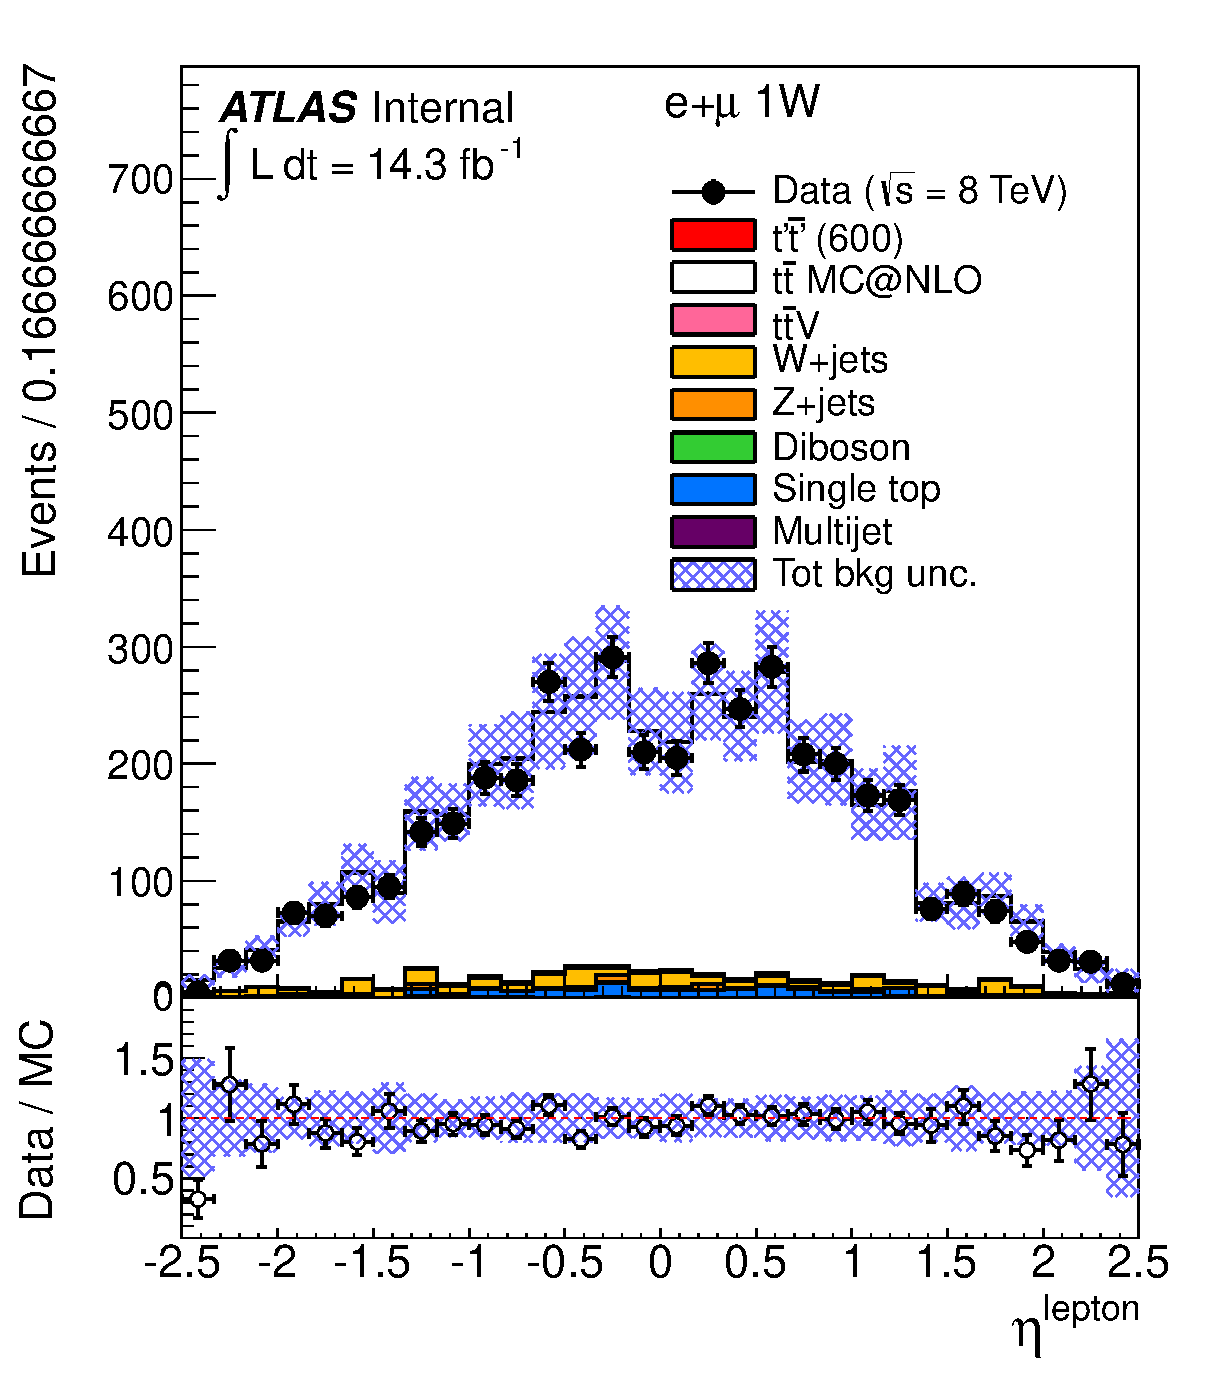
\includegraphics[width=0.30\textwidth]{appendices/figures/sdrs/LepEta_ELEMUONCR5_1W_NOMINAL.eps} &
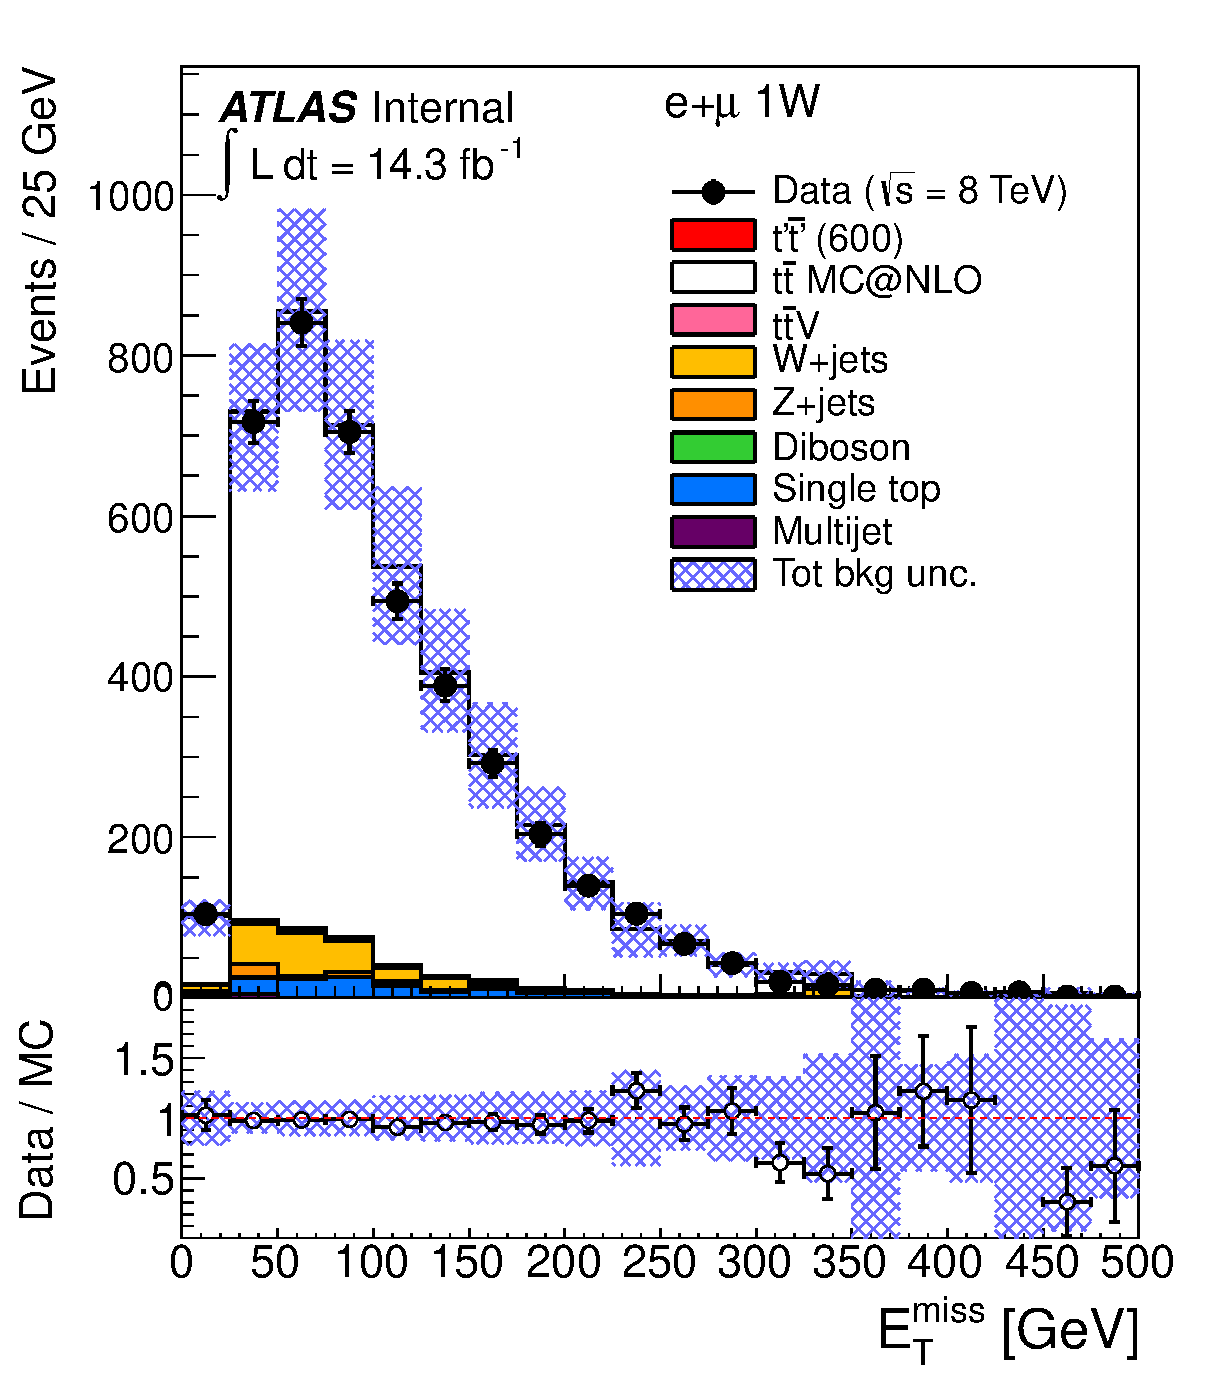
\includegraphics[width=0.30\textwidth]{appendices/figures/sdrs/MET_ELEMUONCR5_1W_NOMINAL.eps} \\
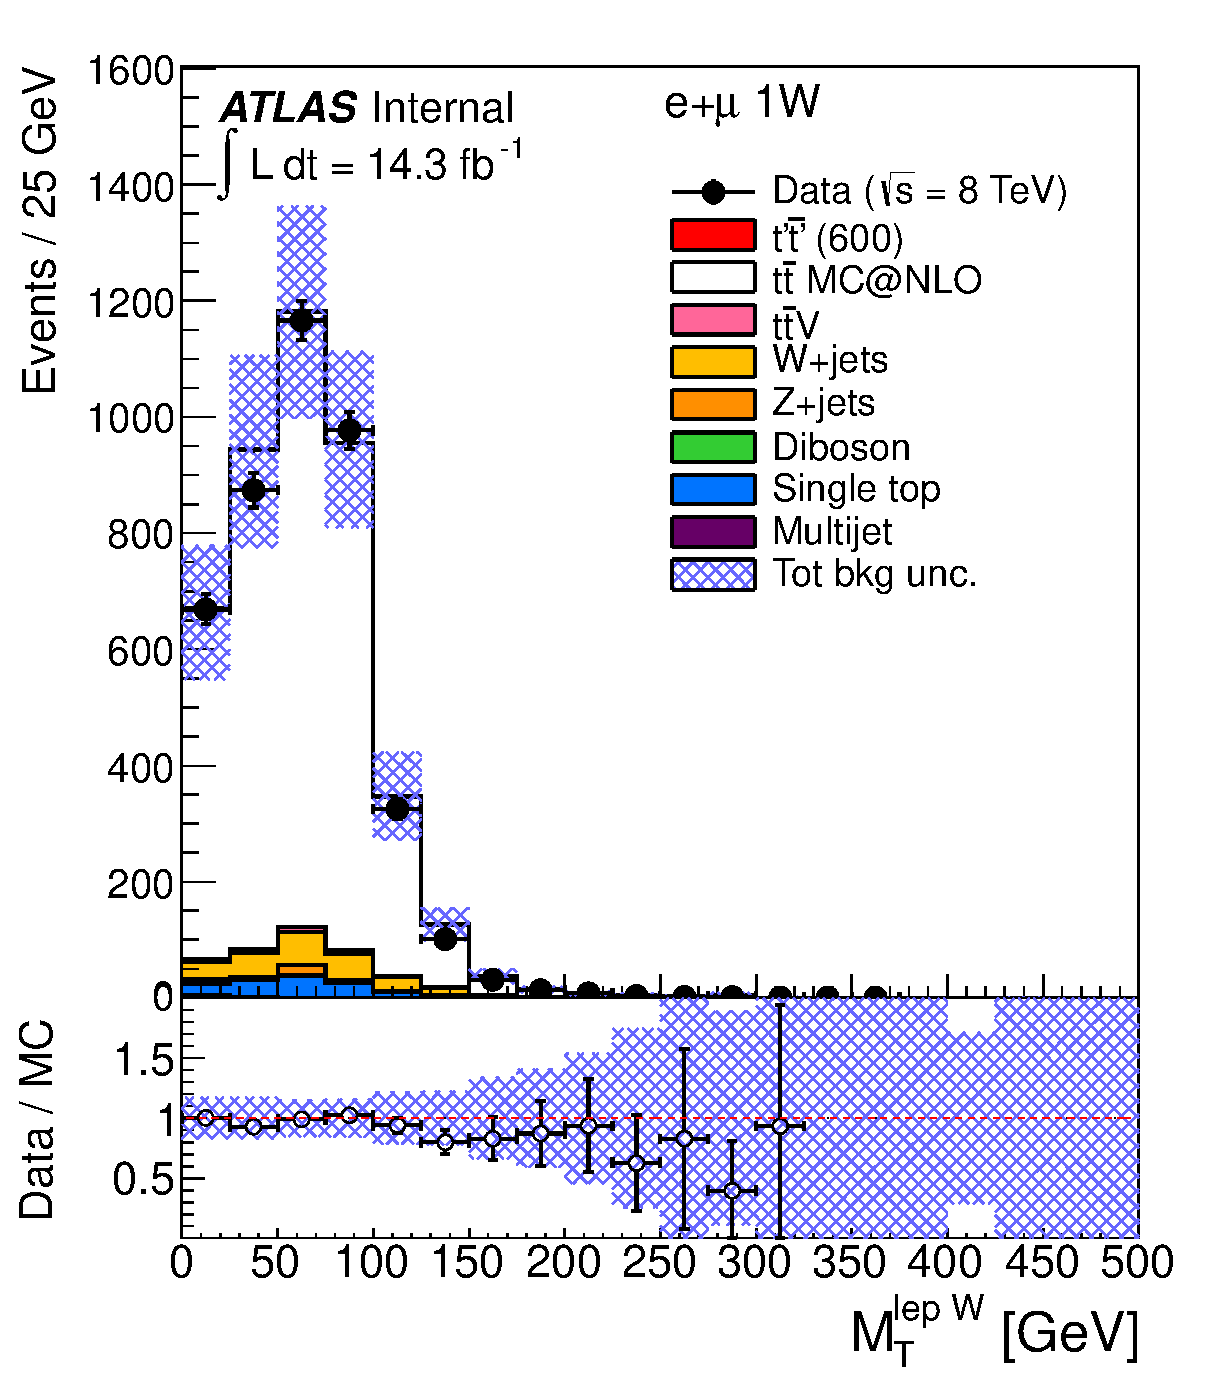
\includegraphics[width=0.30\textwidth]{appendices/figures/sdrs/Wlep_MassT_ELEMUONCR5_1W_NOMINAL.eps} &
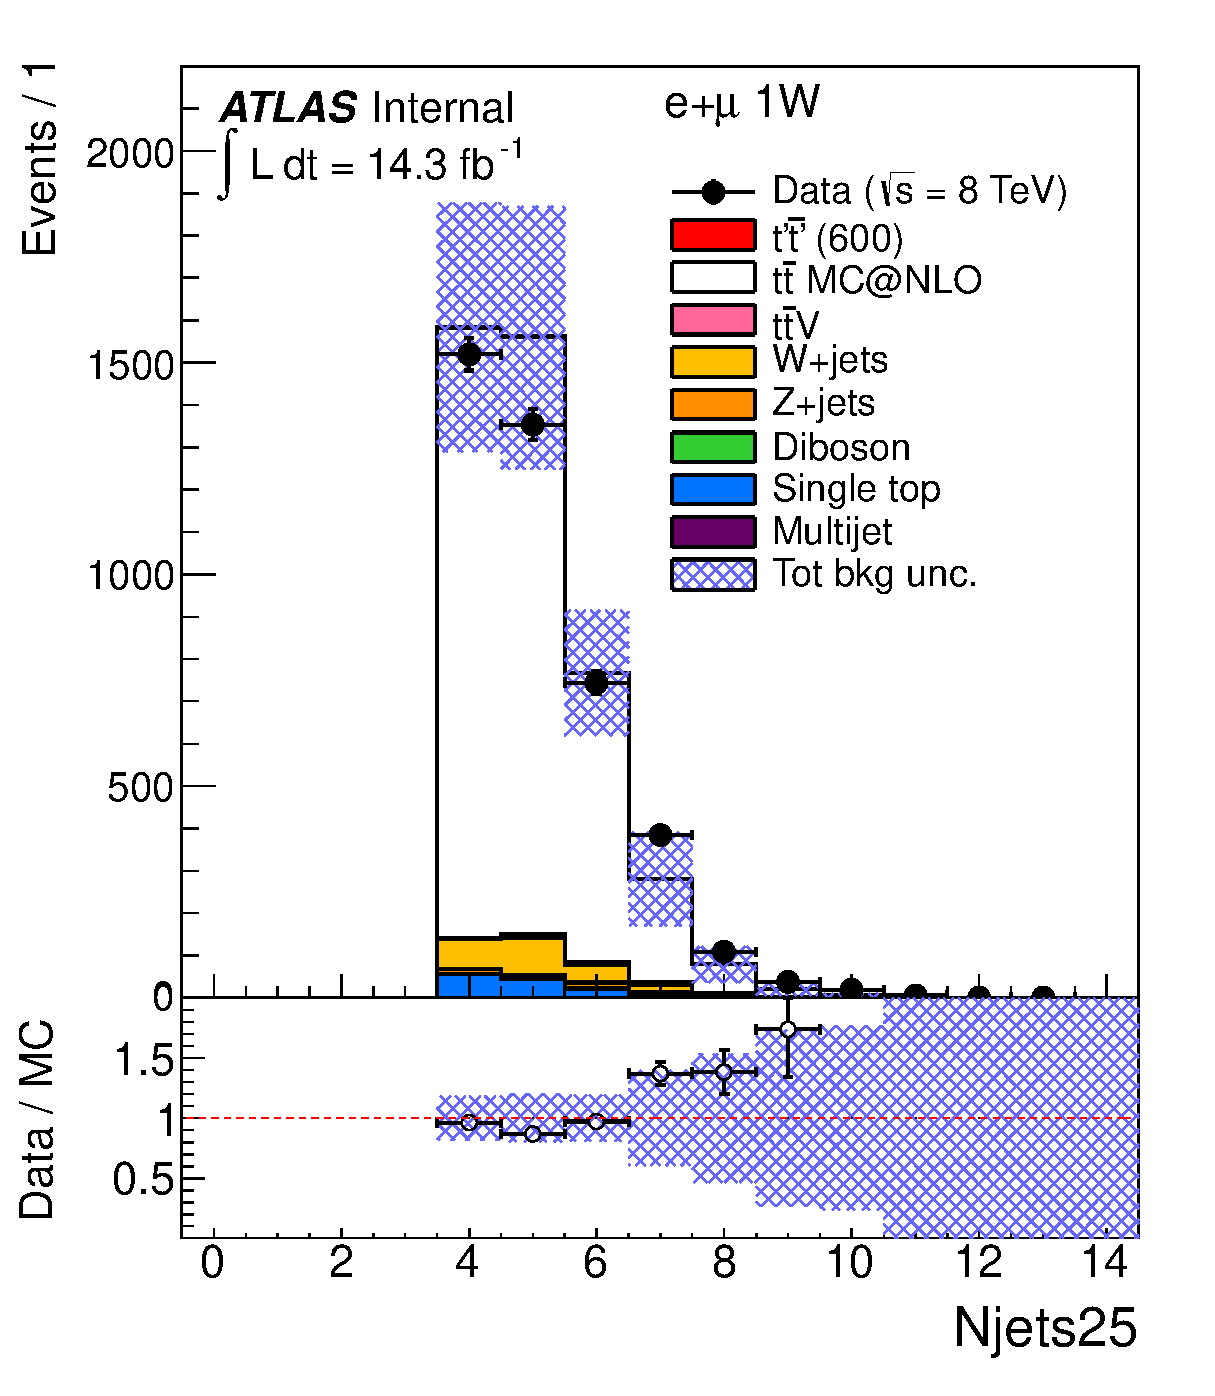
\includegraphics[width=0.30\textwidth]{appendices/figures/sdrs/Njets25_ELEMUONCR5_1W_NOMINAL.eps}  &
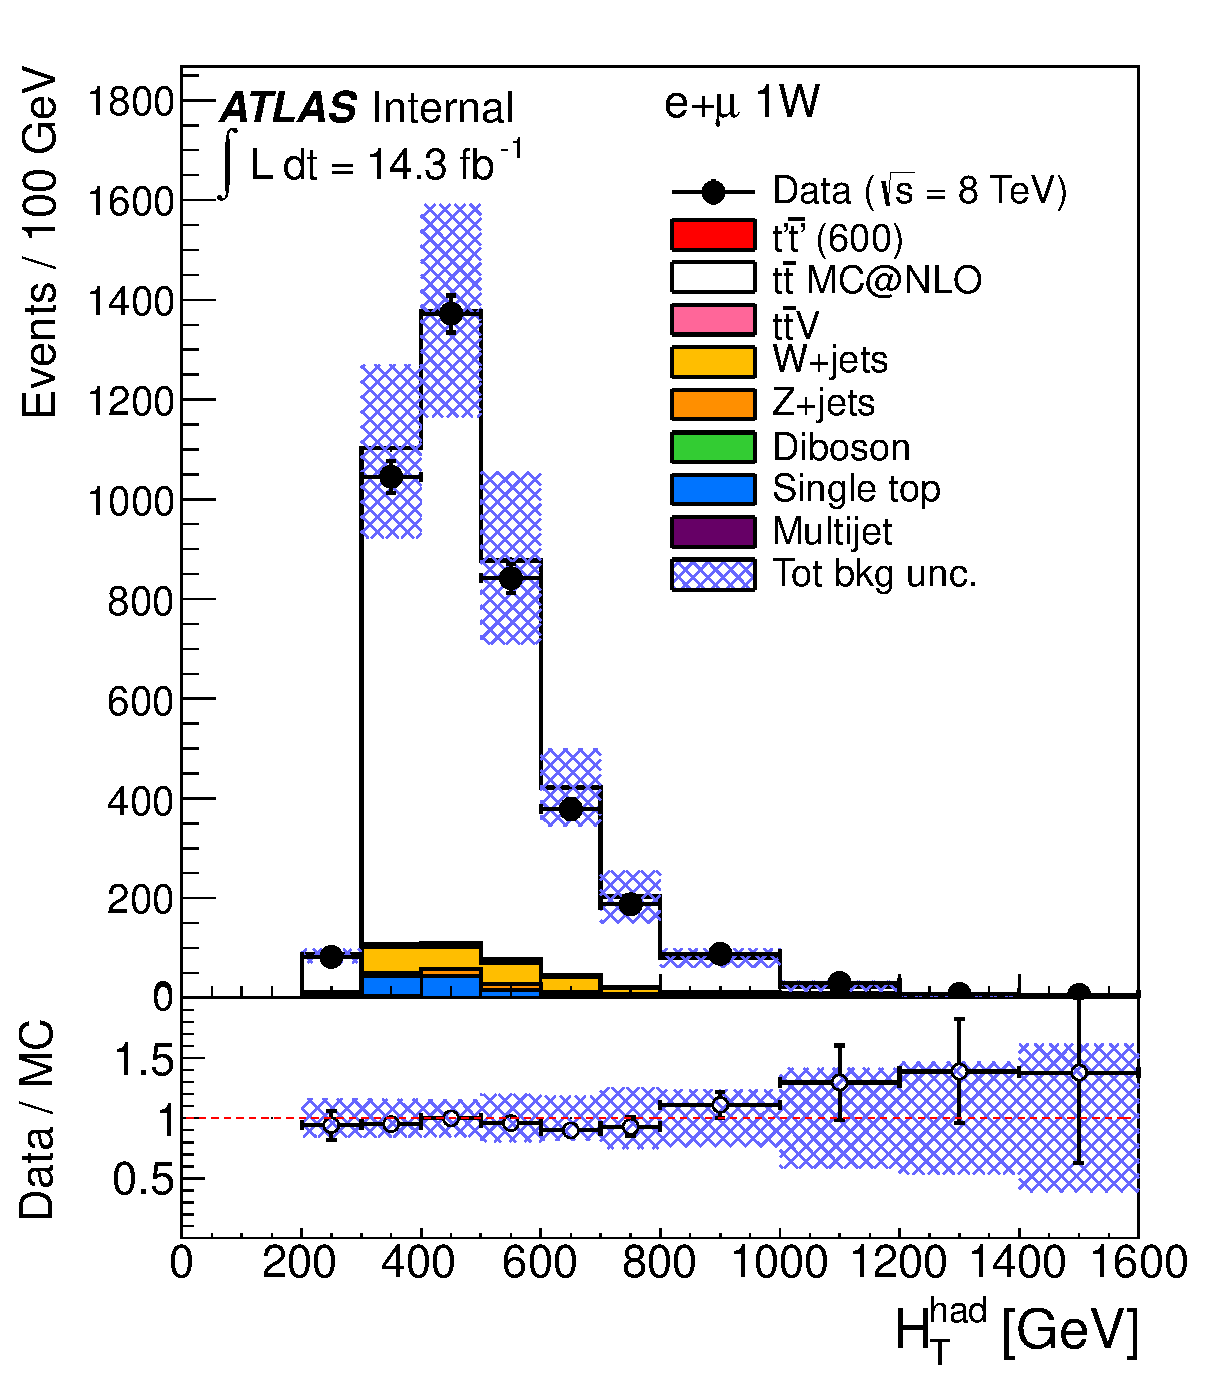
\includegraphics[width=0.30\textwidth]{appendices/figures/sdrs/HTHad_ELEMUONCR5_1W_NOMINAL.eps}  \\
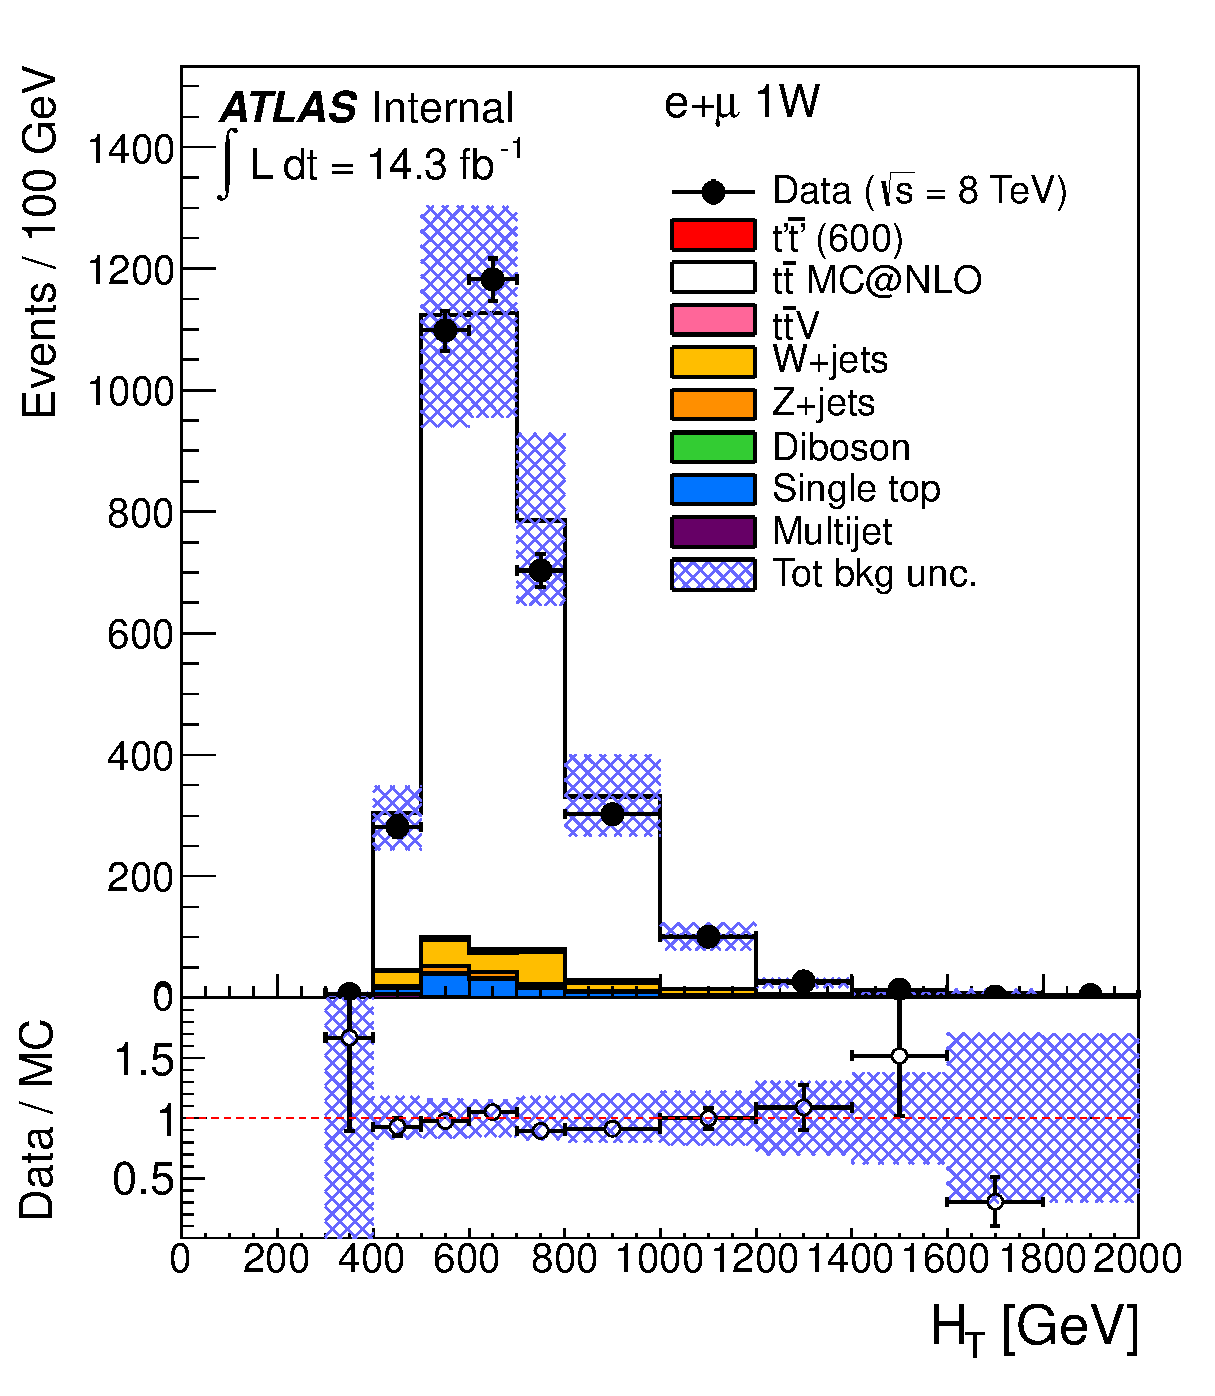
\includegraphics[width=0.30\textwidth]{appendices/figures/sdrs/HTAll_ELEMUONCR5_1W_NOMINAL.eps}  &  &\\
\end{tabular}\caption{\small {Comparison between data and prediction in combined $e$+jets and $\mu$+jets channel in SDR1 (see Sect.~\ref{sec:sdrs} for details) 
for a number of kinematic variables. From top to bottom and left to right, the variables displayed are: lepton $\pt$, lepton $\eta$, missing transverse energy, $W$ transverse mass,
$\hthad$, and $\HT$. The shaded area represents the total background uncertainty.}}
\label{fig:ELEMUONCR5_1}
\end{center}
\end{figure}                                                                             
%%%%%%%%%%%%%%

\clearpage
%%%%%%%%%%%%%%
\begin{figure}[htbp]
\begin{center}
\begin{tabular}{cc}
%
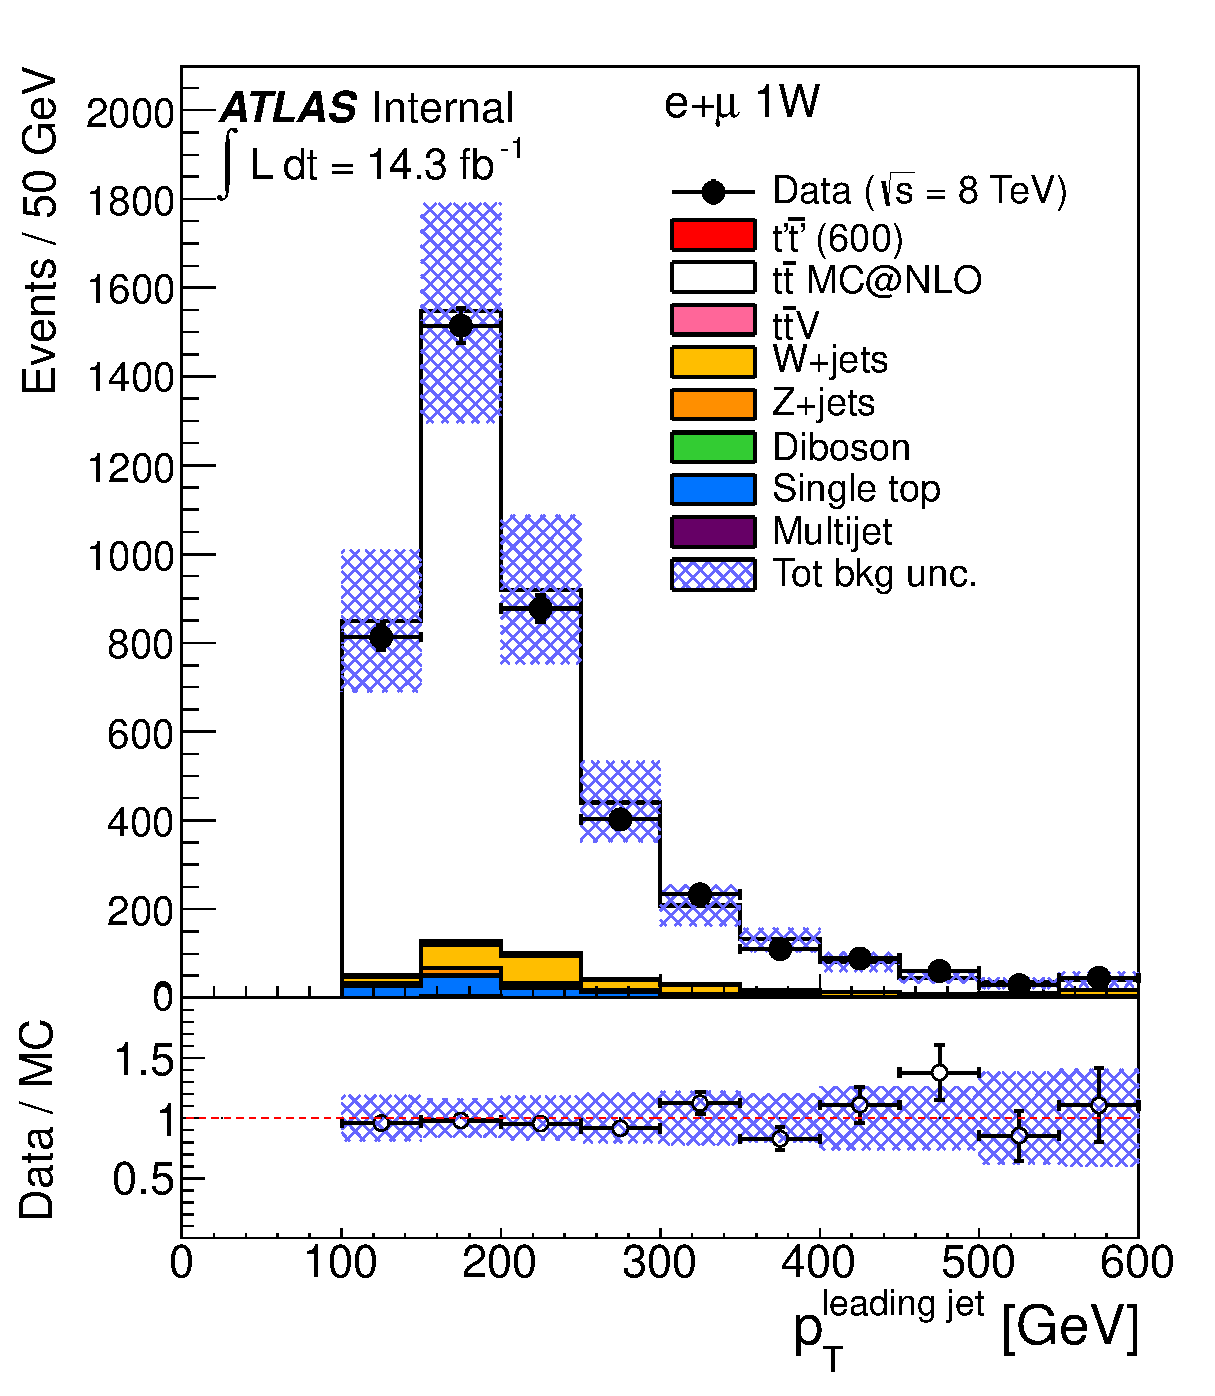
\includegraphics[width=0.30\textwidth]{appendices/figures/sdrs/JetPt1_ELEMUONCR5_1W_NOMINAL.eps} &
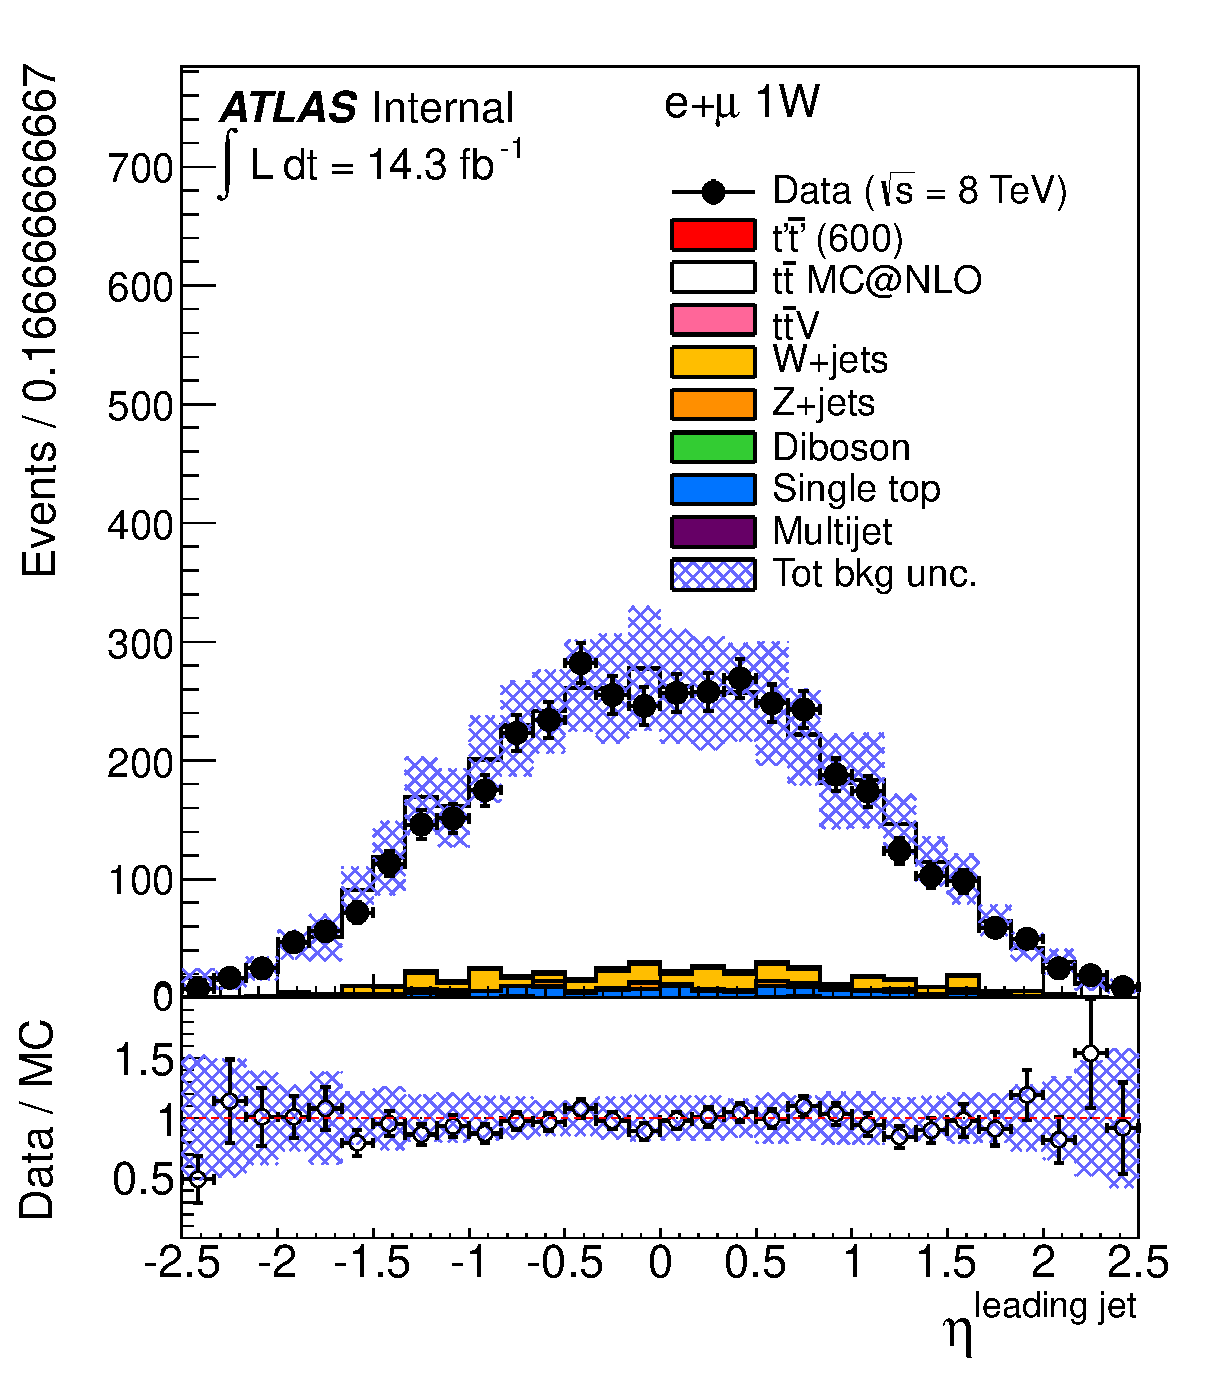
\includegraphics[width=0.30\textwidth]{appendices/figures/sdrs/JetEta1_ELEMUONCR5_1W_NOMINAL.eps} \\
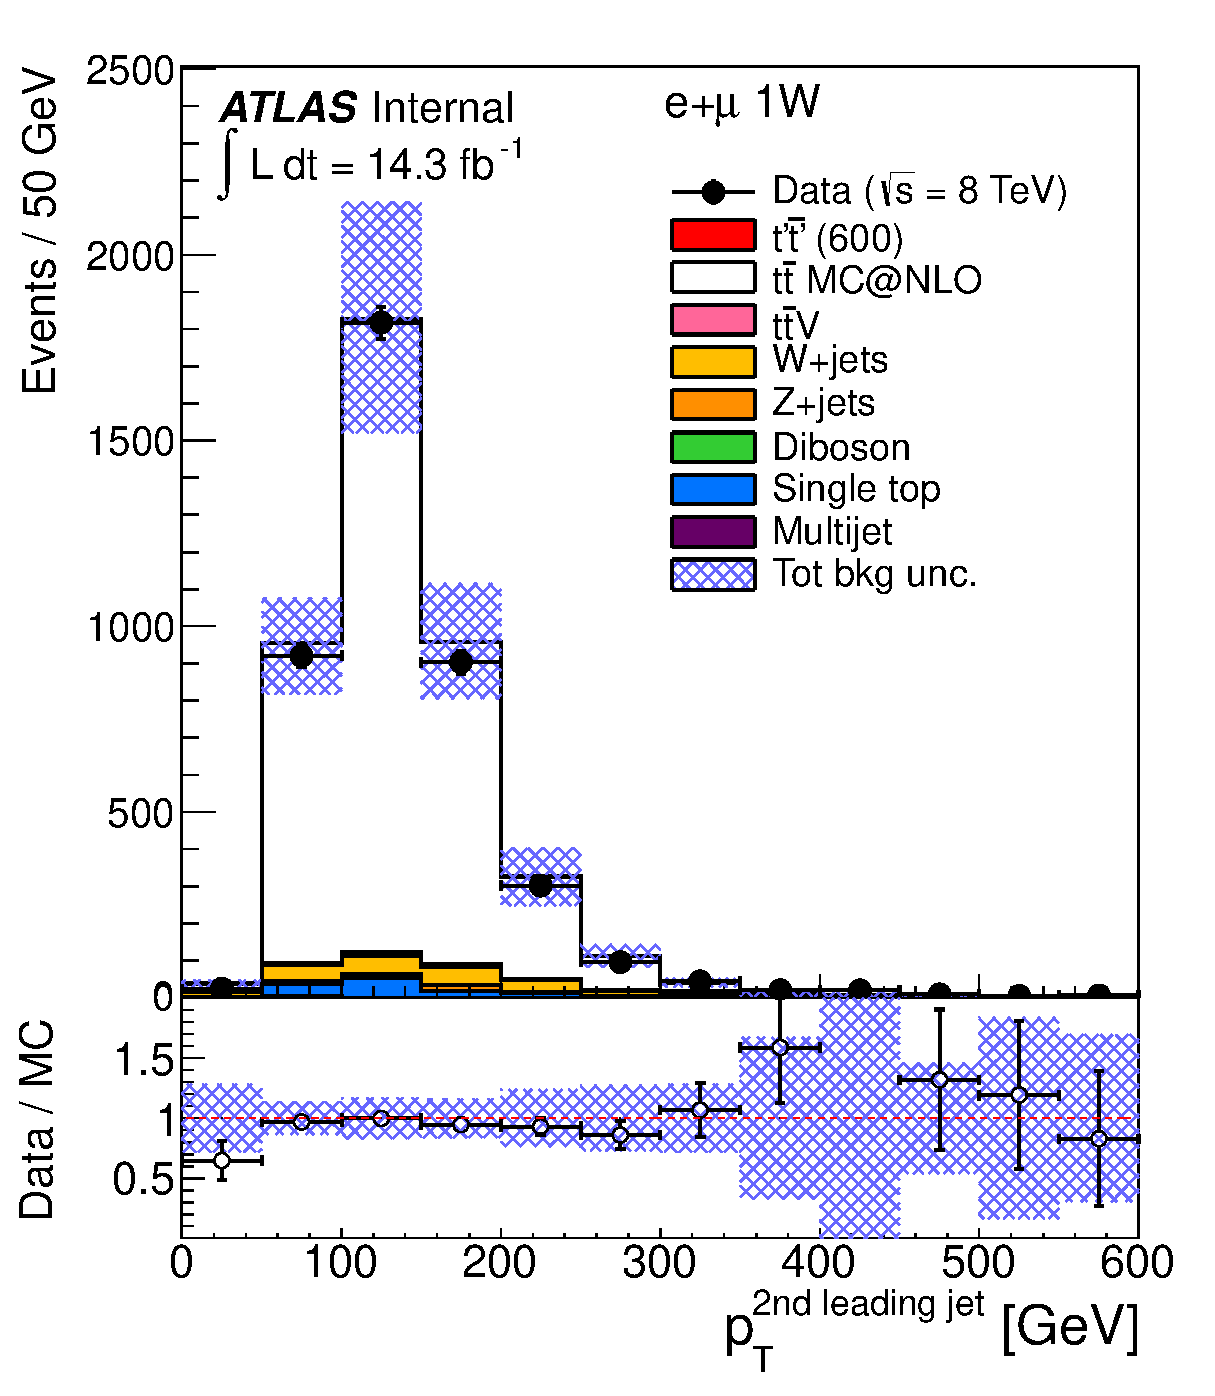
\includegraphics[width=0.30\textwidth]{appendices/figures/sdrs/JetPt2_ELEMUONCR5_1W_NOMINAL.eps} &
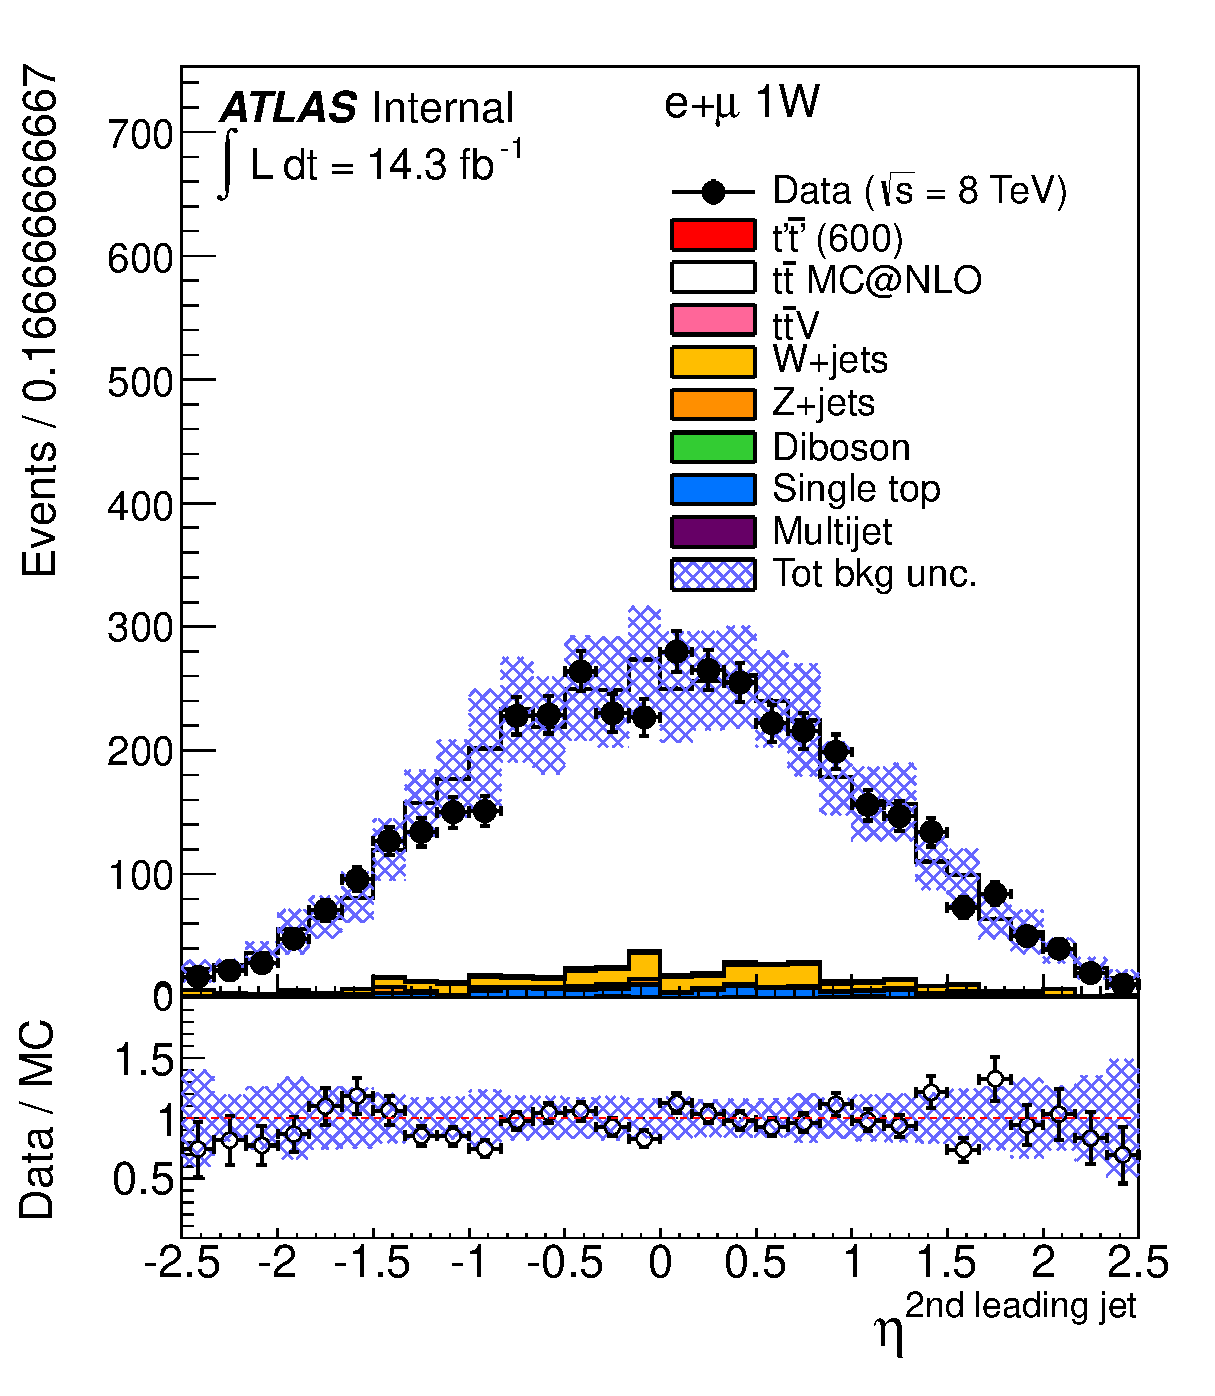
\includegraphics[width=0.30\textwidth]{appendices/figures/sdrs/JetEta2_ELEMUONCR5_1W_NOMINAL.eps} \\
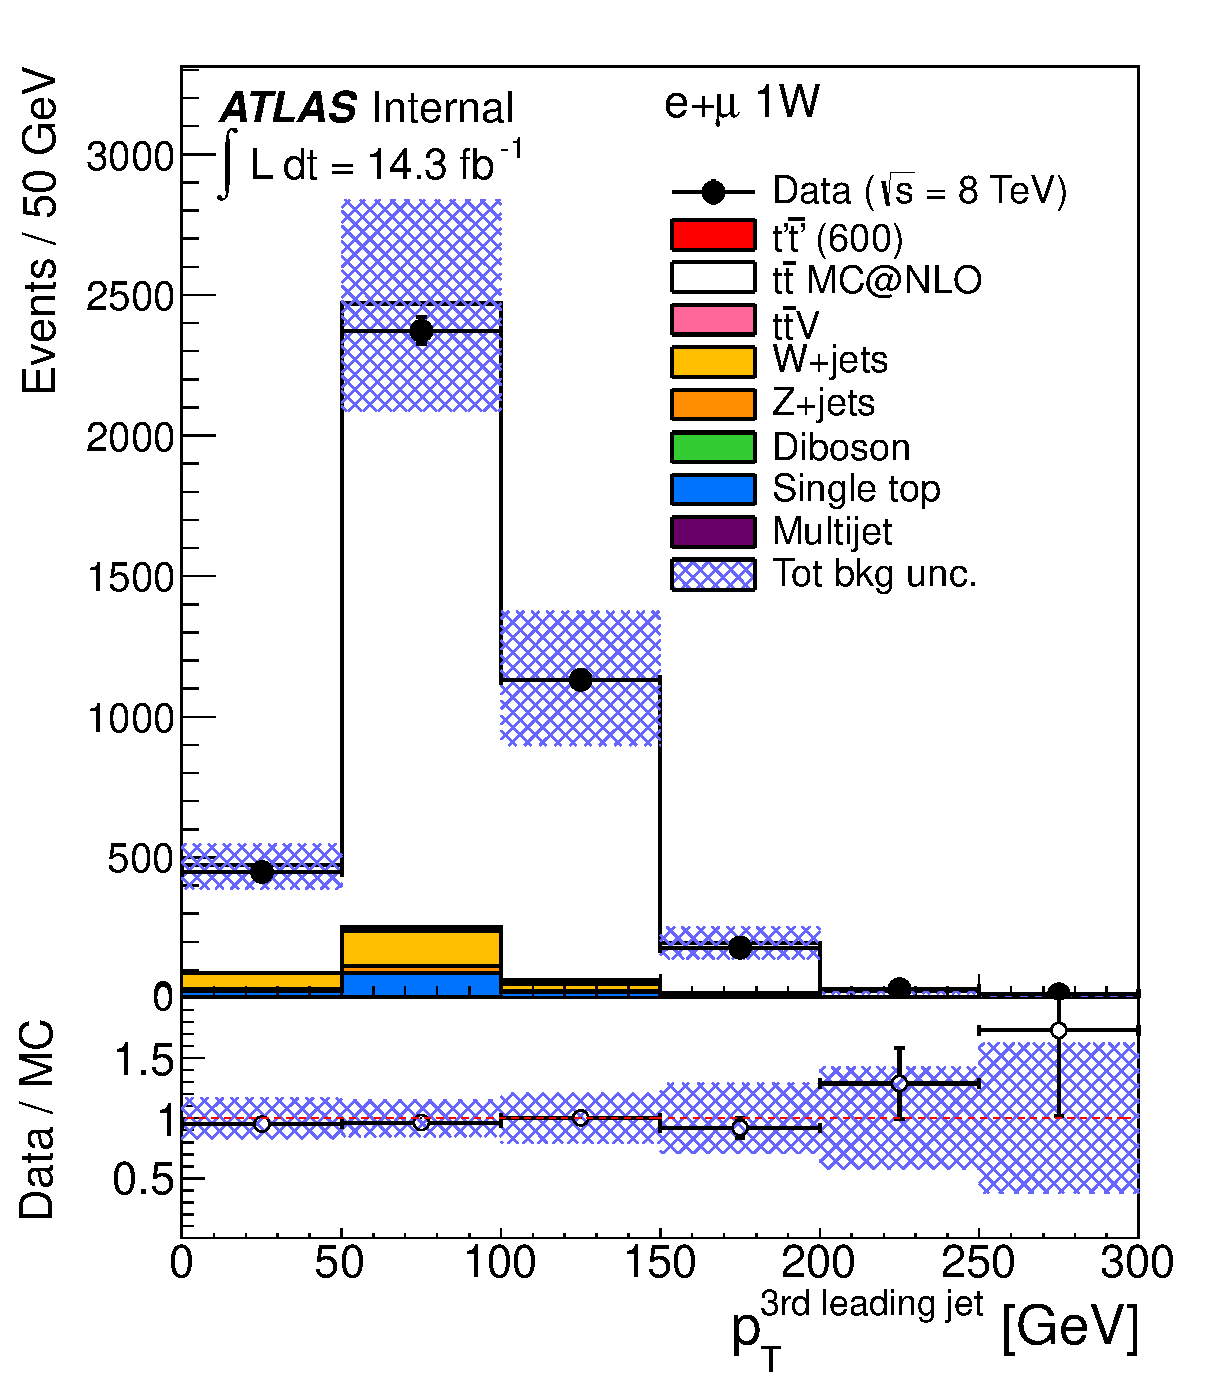
\includegraphics[width=0.30\textwidth]{appendices/figures/sdrs/JetPt3_ELEMUONCR5_1W_NOMINAL.eps} &
\includegraphics[width=0.30\textwidth]{appendices/figures/sdrs/JetEta3_ELEMUONCR5_1W_NOMINAL.eps} \\
\includegraphics[width=0.30\textwidth]{appendices/figures/sdrs/JetPt4_ELEMUONCR5_1W_NOMINAL.eps}  &
\includegraphics[width=0.30\textwidth]{appendices/figures/sdrs/JetEta4_ELEMUONCR5_1W_NOMINAL.eps}  \\
\end{tabular}\caption{\small {Comparison between data and prediction in combined $e$+jets and $\mu$+jets channel in SDR1 (see Sect.~\ref{sec:sdrs} for details) 
for a number of kinematic variables. From top to bottom and left to right, the variables displayed are: leading jet $\pt$ and $\eta$,  second leading jet $\pt$ and $\eta$,
third leading jet $\pt$ and $\eta$, and fourth leading jet $\pt$ and $\eta$. The shaded area represents the total background uncertainty.}}
\label{fig:ELEMUONCR5_2}
\end{center}
\end{figure}                                                                             
%%%%%%%%%%%%%%

\clearpage
%%%%%%%%%%%%%%
\begin{figure}[htbp]
\begin{center}
\begin{tabular}{ccc}
%
\includegraphics[width=0.30\textwidth]{appendices/figures/sdrs/JetPtB1_ELEMUONCR5_1W_NOMINAL.eps}  &
\includegraphics[width=0.30\textwidth]{appendices/figures/sdrs/JetPtB2_ELEMUONCR5_1W_NOMINAL.eps} &
\includegraphics[width=0.30\textwidth]{appendices/figures/sdrs/nWhad_ELEMUONCR5_1W_NOMINAL_logscale.eps} \\
\includegraphics[width=0.30\textwidth]{appendices/figures/sdrs/VLQAna_WbX_W1Pt_ELEMUONCR5_1W_NOMINAL.eps} &
\includegraphics[width=0.30\textwidth]{appendices/figures/sdrs/VLQAna_WbX_DRLepMet_ELEMUONCR5_1W_NOMINAL.eps} &
\includegraphics[width=0.30\textwidth]{appendices/figures/sdrs/VLQAna_WbX_MinDRlb_ELEMUONCR5_1W_NOMINAL.eps} \\
\includegraphics[width=0.30\textwidth]{appendices/figures/sdrs/VLQAna_WbX_MinDRWb_ELEMUONCR5_1W_NOMINAL.eps} &
\includegraphics[width=0.30\textwidth]{appendices/figures/sdrs/VLQAna_WbX_1W_MWb_4_ELEMUONCR5_1W_NOMINAL.eps} & \\
\end{tabular}\caption{\small {Comparison between data and prediction in combined $e$+jets and $\mu$+jets channel in SDR1 (see Sect.~\ref{sec:sdrs} for details) 
for a number of kinematic variables. From top to bottom and left to right, the variables displayed are: $\pt$ for leading and second-leading $b$ jets,
number of $W_{\rm had}$  candidates, $\pt$ of selected $W_{\rm had}$  candidate, $\Delta R(\ell,\nu)$, $\min(\Delta R(\ell, b_{1,2}))$, 
$\min(\Delta R(W_{\rm had}, b_{1,2}))$ and $m_{\rm reco}$.
The shaded area represents the total background uncertainty.}}
\label{fig:ELEMUONCR5_3}
\end{center}
\end{figure}                                                                             
%%%%%%%%%%%%%%

\begin{landscape}
\begin{figure}[htb]\begin{center}
\vskip-1.5cm
\hskip-2cm
\resizebox{1.5\textwidth}{!}{
	\subfigure[]{
          \includegraphics[width=0.3\textwidth]{appendices/figures/sdrs/LepPt_ELEMUONCR5_1W_NOMINAL.eps}}
	\subfigure[]{
          \includegraphics[width=0.3\textwidth]{appendices/figures/sdrs/LepEta_ELEMUONCR5_1W_NOMINAL.eps}}
	\subfigure[]{
          \includegraphics[width=0.3\textwidth]{appendices/figures/sdrs/MET_ELEMUONCR5_1W_NOMINAL.eps}}
	\subfigure[]{
          \includegraphics[width=0.3\textwidth]{appendices/figures/sdrs/Wlep_MassT_ELEMUONCR5_1W_NOMINAL.eps}}
	\subfigure[]{
          \includegraphics[width=0.3\textwidth]{appendices/figures/sdrs/HTAll_ELEMUONCR5_1W_NOMINAL.eps}}
}\\
\hskip-2cm
\resizebox{1.5\textwidth}{!}{
	\subfigure[]{
          \includegraphics[width=0.3\textwidth]{appendices/figures/sdrs/Njets25_ELEMUONCR5_1W_NOMINAL.eps}}
	\subfigure[]{
          \includegraphics[width=0.3\textwidth]{appendices/figures/sdrs/JetPt1_ELEMUONCR5_1W_NOMINAL.eps}}
	\subfigure[]{
          \includegraphics[width=0.3\textwidth]{appendices/figures/sdrs/JetPtB1_ELEMUONCR5_1W_NOMINAL.eps}}
	\subfigure[]{
          \includegraphics[width=0.3\textwidth]{appendices/figures/sdrs/JetPtB2_ELEMUONCR5_1W_NOMINAL.eps}}
	\subfigure[]{
          \includegraphics[width=0.3\textwidth]{appendices/figures/sdrs/nWhad_ELEMUONCR5_1W_NOMINAL.eps}}
}\\
\hskip-2cm
\resizebox{1.5\textwidth}{!}{
	\subfigure[]{
          \includegraphics[width=0.3\textwidth]{appendices/figures/sdrs/VLQAna_WbX_W1Pt_ELEMUONCR5_1W_NOMINAL.eps}}
	\subfigure[]{
          \includegraphics[width=0.3\textwidth]{appendices/figures/sdrs/VLQAna_WbX_DRLepMet_ELEMUONCR5_1W_NOMINAL.eps}}
	\subfigure[]{
          \includegraphics[width=0.3\textwidth]{appendices/figures/sdrs/VLQAna_WbX_MinDRlb_ELEMUONCR5_1W_NOMINAL.eps}}
	\subfigure[]{
          \includegraphics[width=0.3\textwidth]{appendices/figures/sdrs/VLQAna_WbX_MinDRWb_ELEMUONCR5_1W_NOMINAL.eps}}
	\subfigure[]{
          \includegraphics[width=0.3\textwidth]{appendices/figures/sdrs/VLQAna_WbX_1W_MWb_4_ELEMUONCR5_1W_NOMINAL.eps}}
}
	\caption{Comparison between data and prediction in the electron and muon combined channel in SDR1
          for a number of kinematic variables: 
          %%%row 1
          (a)  lepton $\pt$, (b) lepton $\eta$, (c) missing transverse energy, 
          (d)  $W$ transverse mass, (e) $\HT$ variable, 
          %%%row 2
          (f) number of jets with $\pt>25\gev$, (g) leading jet $\pt$, 
          (h) $\pt$ for leading \bjet, (i) $\pt$ for second-leading \bjet,
          (j) number of $W_{\rm had}$  candidates, 
          %%%row 3
          (k) $\pt$ of selected $W_{\rm had}$  candidate, 
          (l) $\Delta R(\ell,\nu)$, (m) $\min(\Delta R(\ell, b_{1,2}))$, 
          (n) $\min(\Delta R(W_{\rm had}, b_{1,2}))$ and (o) $m_{\rm reco}$.
          The shaded area represents the total background uncertainty.\label{fig:ELEMUONCR5}}
\end{center}\end{figure}
\end{landscape}


\clearpage

\section{Comparison between data and prediction in SDR2}
\label{sec:DataMC_CR1}

SDR2: {\sl loose} selection with reversed $\HT$ cut (i.e. $\HT<800\gev$).

%%%%%%%%%%%%%%%
\begin{table}[h!]
\begin{center}
\renewcommand{\arraystretch}{1.3}
\begin{tabular}{l*{1}{r@{ $\pm$ }r@{ }l}}
\hline\hline
 & \multicolumn{3}{c}{ELEMUONCR1\_1W}\\
\hline
$T\bar{T}(600\GeV)$ (Chiral) & $0.73$ & $0.31$ & $^{+0.40}_{-0.45}$\\
\hline
$t\bar{t}$ & $72.59$ & $5.46$ & $^{+18.64}_{-18.93}$\\
$W$+jets & $6.46$ & $5.61$ & $^{+2.77}_{-6.57}$\\
$Z$+jets & $0.91$ & $0.91$ & $^{+1.01}_{-1.36}$\\
Diboson & $0.10$ & $0.08$ & $^{+0.02}_{-0.02}$\\
Single top & $1.13$ & $0.57$ & $^{+1.38}_{-0.42}$\\
$t\bar{t}$$V$ & $0.47$ & $0.05$ & $^{+0.20}_{-0.18}$\\
Multijet & $0.36$ & $0.66$ & $ \pm\ 0.18$\\
\hline
Total bkg. & $82.01 $ & $ 7.93$ & $ ^{+20.71}_{-23.47}$\\
\hline
Data & \multicolumn{3}{c}{$85$}\\
\hline\hline
\end{tabular}

\vspace{0.5cm}

\caption{\small{Number of observed events compared to the SM expectation for
the combined electron and muon channels in SDR2 (see Section~\ref{sec:wbxCR} for details) . 
The expected signal yield assuming $m_{\T}=600\gev$ for the chiral scenario is also shown. 
The quoted uncertainties include both statistical and systematic contributions.}}
\label{tab:CR1_1W_evtable}
\end{center}
\end{table}
%%%%%%%%%%%%%%%

\clearpage

%%%%%%%%%%%%%%%
\begin{figure}[h!]
\begin{center}
\begin{tabular}{ccc}
%
\includegraphics[width=0.30\textwidth]{appendices/figures/sdrs/LepPt_ELEMUONCR1_1W_NOMINAL.eps} &
\includegraphics[width=0.30\textwidth]{appendices/figures/sdrs/LepEta_ELEMUONCR1_1W_NOMINAL.eps} &
\includegraphics[width=0.30\textwidth]{appendices/figures/sdrs/MET_ELEMUONCR1_1W_NOMINAL.eps} \\
\includegraphics[width=0.30\textwidth]{appendices/figures/sdrs/Wlep_MassT_ELEMUONCR1_1W_NOMINAL.eps} &
\includegraphics[width=0.30\textwidth]{appendices/figures/sdrs/Njets25_ELEMUONCR1_1W_NOMINAL.eps}  &
\includegraphics[width=0.30\textwidth]{appendices/figures/sdrs/HTHad_ELEMUONCR1_1W_NOMINAL.eps}  \\
\includegraphics[width=0.30\textwidth]{appendices/figures/sdrs/HTAll_ELEMUONCR1_1W_NOMINAL.eps}  &  &\\
\end{tabular}\caption{\small {Comparison between data and prediction in combined $e$+jets and $\mu$+jets channel in SDR2 (see Sect.~\ref{sec:sdrs} for details) 
for a number of kinematic variables. From top to bottom and left to right, the variables displayed are: lepton $\pt$, lepton $\eta$, missing transverse energy, $W$ transverse mass,
$\hthad$, and $\HT$. The shaded area represents the total background uncertainty.}}
\label{fig:ELEMUONCR1_1}
\end{center}
\end{figure}                                                                             
%%%%%%%%%%%%%%

\clearpage
%%%%%%%%%%%%%%
\begin{figure}[htbp]
\begin{center}
\begin{tabular}{cc}
%
\includegraphics[width=0.30\textwidth]{appendices/figures/sdrs/JetPt1_ELEMUONCR1_1W_NOMINAL.eps} &
\includegraphics[width=0.30\textwidth]{appendices/figures/sdrs/JetEta1_ELEMUONCR1_1W_NOMINAL.eps} \\
\includegraphics[width=0.30\textwidth]{appendices/figures/sdrs/JetPt2_ELEMUONCR1_1W_NOMINAL.eps} &
\includegraphics[width=0.30\textwidth]{appendices/figures/sdrs/JetEta2_ELEMUONCR1_1W_NOMINAL.eps} \\
\includegraphics[width=0.30\textwidth]{appendices/figures/sdrs/JetPt3_ELEMUONCR1_1W_NOMINAL.eps} &
\includegraphics[width=0.30\textwidth]{appendices/figures/sdrs/JetEta3_ELEMUONCR1_1W_NOMINAL.eps} \\
\includegraphics[width=0.30\textwidth]{appendices/figures/sdrs/JetPt4_ELEMUONCR1_1W_NOMINAL.eps}  &
\includegraphics[width=0.30\textwidth]{appendices/figures/sdrs/JetEta4_ELEMUONCR1_1W_NOMINAL.eps}  \\
\end{tabular}\caption{\small {Comparison between data and prediction in combined $e$+jets and $\mu$+jets channel in SDR2 (see Sect.~\ref{sec:sdrs} for details) 
for a number of kinematic variables. From top to bottom and left to right, the variables displayed are: leading jet $\pt$ and $\eta$,  second leading jet $\pt$ and $\eta$,
third leading jet $\pt$ and $\eta$, and fourth leading jet $\pt$ and $\eta$. The shaded area represents the total background uncertainty.}}
\label{fig:ELEMUONCR1_2}
\end{center}
\end{figure}                                                                             
%%%%%%%%%%%%%%

\clearpage
%%%%%%%%%%%%%%
\begin{figure}[htbp]
\begin{center}
\begin{tabular}{ccc}
%
\includegraphics[width=0.30\textwidth]{appendices/figures/sdrs/JetPtB1_ELEMUONCR1_1W_NOMINAL.eps}  &
\includegraphics[width=0.30\textwidth]{appendices/figures/sdrs/JetPtB2_ELEMUONCR1_1W_NOMINAL.eps} &
\includegraphics[width=0.30\textwidth]{appendices/figures/sdrs/nWhad_ELEMUONCR1_1W_NOMINAL_logscale.eps} \\
\includegraphics[width=0.30\textwidth]{appendices/figures/sdrs/VLQAna_WbX_W1Pt_ELEMUONCR1_1W_NOMINAL.eps} &
\includegraphics[width=0.30\textwidth]{appendices/figures/sdrs/VLQAna_WbX_DRLepMet_ELEMUONCR1_1W_NOMINAL.eps} &
\includegraphics[width=0.30\textwidth]{appendices/figures/sdrs/VLQAna_WbX_MinDRlb_ELEMUONCR1_1W_NOMINAL.eps} \\
\includegraphics[width=0.30\textwidth]{appendices/figures/sdrs/VLQAna_WbX_MinDRWb_ELEMUONCR1_1W_NOMINAL.eps} &
\includegraphics[width=0.30\textwidth]{appendices/figures/sdrs/VLQAna_WbX_1W_MWb_4_ELEMUONCR1_1W_NOMINAL.eps} & \\
\end{tabular}\caption{\small {Comparison between data and prediction in combined $e$+jets and $\mu$+jets channel in SDR2 (see Sect.~\ref{sec:sdrs} for details) 
for a number of kinematic variables. From top to bottom and left to right, the variables displayed are: $\pt$ for leading and second-leading $b$ jets,
number of $W_{\rm had}$  candidates, $\pt$ of selected $W_{\rm had}$  candidate, $\Delta R(\ell,\nu)$, $\min(\Delta R(\ell, b_{1,2}))$, 
$\min(\Delta R(W_{\rm had}, b_{1,2}))$ and $m_{\rm reco}$.
The shaded area represents the total background uncertainty.}}
\label{fig:ELEMUONCR1_3}
\end{center}
\end{figure}                                                                             
%%%%%%%%%%%%%%

\begin{landscape}
\begin{figure}[htb]\begin{center}
\vskip-1.5cm
\hskip-2cm
\resizebox{1.5\textwidth}{!}{
	\subfigure[]{
          \includegraphics[width=0.3\textwidth]{appendices/figures/sdrs/LepPt_ELEMUONCR1_1W_NOMINAL.eps}}
	\subfigure[]{
          \includegraphics[width=0.3\textwidth]{appendices/figures/sdrs/LepEta_ELEMUONCR1_1W_NOMINAL.eps}}
	\subfigure[]{
          \includegraphics[width=0.3\textwidth]{appendices/figures/sdrs/MET_ELEMUONCR1_1W_NOMINAL.eps}}
	\subfigure[]{
          \includegraphics[width=0.3\textwidth]{appendices/figures/sdrs/Wlep_MassT_ELEMUONCR1_1W_NOMINAL.eps}}
	\subfigure[]{
          \includegraphics[width=0.3\textwidth]{appendices/figures/sdrs/HTAll_ELEMUONCR1_1W_NOMINAL.eps}}
}\\
\hskip-2cm
\resizebox{1.5\textwidth}{!}{
	\subfigure[]{
          \includegraphics[width=0.3\textwidth]{appendices/figures/sdrs/Njets25_ELEMUONCR1_1W_NOMINAL.eps}}
	\subfigure[]{
          \includegraphics[width=0.3\textwidth]{appendices/figures/sdrs/JetPt1_ELEMUONCR1_1W_NOMINAL.eps}}
	\subfigure[]{
          \includegraphics[width=0.3\textwidth]{appendices/figures/sdrs/JetPtB1_ELEMUONCR1_1W_NOMINAL.eps}}
	\subfigure[]{
          \includegraphics[width=0.3\textwidth]{appendices/figures/sdrs/JetPtB2_ELEMUONCR1_1W_NOMINAL.eps}}
	\subfigure[]{
          \includegraphics[width=0.3\textwidth]{appendices/figures/sdrs/nWhad_ELEMUONCR1_1W_NOMINAL.eps}}
}\\
\hskip-2cm
\resizebox{1.5\textwidth}{!}{
	\subfigure[]{
          \includegraphics[width=0.3\textwidth]{appendices/figures/sdrs/VLQAna_WbX_W1Pt_ELEMUONCR1_1W_NOMINAL.eps}}
	\subfigure[]{
          \includegraphics[width=0.3\textwidth]{appendices/figures/sdrs/VLQAna_WbX_DRLepMet_ELEMUONCR1_1W_NOMINAL.eps}}
	\subfigure[]{
          \includegraphics[width=0.3\textwidth]{appendices/figures/sdrs/VLQAna_WbX_MinDRlb_ELEMUONCR1_1W_NOMINAL.eps}}
	\subfigure[]{
          \includegraphics[width=0.3\textwidth]{appendices/figures/sdrs/VLQAna_WbX_MinDRWb_ELEMUONCR1_1W_NOMINAL.eps}}
	\subfigure[]{
          \includegraphics[width=0.3\textwidth]{appendices/figures/sdrs/VLQAna_WbX_1W_MWb_4_ELEMUONCR1_1W_NOMINAL.eps}}
}
	\caption{Comparison between data and prediction in combined $e$+jets and $\mu$+jets combined channel in SDR2
          for a number of kinematic variables: 
          %%%row 1
          (a)  lepton $\pt$, (b) lepton $\eta$, (c) missing transverse energy, 
          (d)  $W$ transverse mass, (e) $\HT$ variable, 
          %%%row 2
          (f) number of jets with $\pt>25\gev$, (g) leading jet $\pt$, 
          (h) $\pt$ for leading \bjet, (i) $\pt$ for second-leading \bjet,
          (j) number of $W_{\rm had}$  candidates, 
          %%%row 3
          (k) $\pt$ of selected $W_{\rm had}$  candidate, 
          (l) $\Delta R(\ell,\nu)$, (m) $\min(\Delta R(\ell, b_{1,2}))$, 
          (n) $\min(\Delta R(W_{\rm had}, b_{1,2}))$ and (o) $m_{\rm reco}$.
          The shaded area represents the total background uncertainty.\label{fig:ELEMUONCR1}}
\end{center}\end{figure}
\end{landscape}


\clearpage

\section{Comparison between data and prediction in SDR3}
\label{sec:DataMC_CR2}

SDR3: {\sl loose} selection with reversed $b$-jet $\pt$ cuts (i.e. $\pt < 160\gev$ and $\pt < 80\gev$).

%%%%%%%%%%%%%%%
\begin{table}[h!]
\begin{center}
\renewcommand{\arraystretch}{1.3}
\begin{tabular}{l*{1}{r@{ $\pm$ }r@{ }l}}
\hline\hline
 & \multicolumn{3}{c}{ELEMUONCR2\_1W}\\
\hline
$T\bar{T}(600\GeV)$ (Chiral) & $12.84$ & $1.28$ & $^{+3.53}_{-5.30}$\\
\hline
$t\bar{t}$ & $472.53$ & $14.37$ & $^{+119.04}_{-117.67}$\\
$W$+jets & $92.31$ & $16.04$ & $^{+52.50}_{-43.49}$\\
$Z$+jets & $7.52$ & $2.77$ & $^{+5.81}_{-4.95}$\\
Diboson & $1.81$ & $0.45$ & $^{+0.18}_{-0.45}$\\
Single top & $39.14$ & $3.73$ & $^{+9.44}_{-6.71}$\\
$t\bar{t}$$V$ & $8.87$ & $0.23$ & $^{+3.03}_{-2.93}$\\
Multijet & $-3.68$ & $2.63$ & $ \pm\ 0.00$\\
\hline
Total bkg. & $618.50 $ & $ 22.19$ & $ ^{+167.53}_{-149.64}$\\
\hline
Data & \multicolumn{3}{c}{$661$}\\
\hline\hline
\end{tabular}

\vspace{0.5cm}

\caption{\small{Number of observed events compared to the SM expectation for
the combined electron and muon channels in SDR3 (see Section~\ref{sec:wbxCR} for details) . 
The expected signal yield assuming $m_{\T}=600\gev$ for the chiral scenario is also shown. 
The quoted uncertainties include both statistical and systematic contributions.}}
\label{tab:CR2_1W_evtable}
\end{center}
\end{table}
%%%%%%%%%%%%%%%

\clearpage

%%%%%%%%%%%%%%%
\begin{figure}[h!]
\begin{center}
\begin{tabular}{ccc}
%
\includegraphics[width=0.30\textwidth]{appendices/figures/sdrs/LepPt_ELEMUONCR2_1W_NOMINAL.eps} &
\includegraphics[width=0.30\textwidth]{appendices/figures/sdrs/LepEta_ELEMUONCR2_1W_NOMINAL.eps} &
\includegraphics[width=0.30\textwidth]{appendices/figures/sdrs/MET_ELEMUONCR2_1W_NOMINAL.eps} \\
\includegraphics[width=0.30\textwidth]{appendices/figures/sdrs/Wlep_MassT_ELEMUONCR2_1W_NOMINAL.eps} &
\includegraphics[width=0.30\textwidth]{appendices/figures/sdrs/Njets25_ELEMUONCR2_1W_NOMINAL.eps}  &
\includegraphics[width=0.30\textwidth]{appendices/figures/sdrs/HTHad_ELEMUONCR2_1W_NOMINAL.eps}  \\
\includegraphics[width=0.30\textwidth]{appendices/figures/sdrs/HTAll_ELEMUONCR2_1W_NOMINAL.eps}  &  &\\
\end{tabular}\caption{\small {Comparison between data and prediction in combined $e$+jets and $\mu$+jets channel in SDR3 (see Sect.~\ref{sec:sdrs} for details) 
for a number of kinematic variables. From top to bottom and left to right, the variables displayed are: lepton $\pt$, lepton $\eta$, missing transverse energy, $W$ transverse mass,
$\hthad$, and $\HT$. The shaded area represents the total background uncertainty.}}
\label{fig:ELEMUONCR2_1}
\end{center}
\end{figure}                                                                             
%%%%%%%%%%%%%%

\clearpage
%%%%%%%%%%%%%%
\begin{figure}[htbp]
\begin{center}
\begin{tabular}{cc}
%
\includegraphics[width=0.30\textwidth]{appendices/figures/sdrs/JetPt1_ELEMUONCR2_1W_NOMINAL.eps} &
\includegraphics[width=0.30\textwidth]{appendices/figures/sdrs/JetEta1_ELEMUONCR2_1W_NOMINAL.eps} \\
\includegraphics[width=0.30\textwidth]{appendices/figures/sdrs/JetPt2_ELEMUONCR2_1W_NOMINAL.eps} &
\includegraphics[width=0.30\textwidth]{appendices/figures/sdrs/JetEta2_ELEMUONCR2_1W_NOMINAL.eps} \\
\includegraphics[width=0.30\textwidth]{appendices/figures/sdrs/JetPt3_ELEMUONCR2_1W_NOMINAL.eps} &
\includegraphics[width=0.30\textwidth]{appendices/figures/sdrs/JetEta3_ELEMUONCR2_1W_NOMINAL.eps} \\
\includegraphics[width=0.30\textwidth]{appendices/figures/sdrs/JetPt4_ELEMUONCR2_1W_NOMINAL.eps}  &
\includegraphics[width=0.30\textwidth]{appendices/figures/sdrs/JetEta4_ELEMUONCR2_1W_NOMINAL.eps}  \\
\end{tabular}\caption{\small {Comparison between data and prediction in combined $e$+jets and $\mu$+jets channel in SDR3 (see Sect.~\ref{sec:sdrs} for details) 
for a number of kinematic variables. From top to bottom and left to right, the variables displayed are: leading jet $\pt$ and $\eta$,  second leading jet $\pt$ and $\eta$,
third leading jet $\pt$ and $\eta$, and fourth leading jet $\pt$ and $\eta$. The shaded area represents the total background uncertainty.}}
\label{fig:ELEMUONCR2_2}
\end{center}
\end{figure}                                                                             
%%%%%%%%%%%%%%

\clearpage
%%%%%%%%%%%%%%
\begin{figure}[htbp]
\begin{center}
\begin{tabular}{ccc}
%
\includegraphics[width=0.30\textwidth]{appendices/figures/sdrs/JetPtB1_ELEMUONCR2_1W_NOMINAL.eps}  &
\includegraphics[width=0.30\textwidth]{appendices/figures/sdrs/JetPtB2_ELEMUONCR2_1W_NOMINAL.eps} &
\includegraphics[width=0.30\textwidth]{appendices/figures/sdrs/nWhad_ELEMUONCR2_1W_NOMINAL_logscale.eps} \\
\includegraphics[width=0.30\textwidth]{appendices/figures/sdrs/VLQAna_WbX_W1Pt_ELEMUONCR2_1W_NOMINAL.eps} &
\includegraphics[width=0.30\textwidth]{appendices/figures/sdrs/VLQAna_WbX_DRLepMet_ELEMUONCR2_1W_NOMINAL.eps} &
\includegraphics[width=0.30\textwidth]{appendices/figures/sdrs/VLQAna_WbX_MinDRlb_ELEMUONCR2_1W_NOMINAL.eps} \\
\includegraphics[width=0.30\textwidth]{appendices/figures/sdrs/VLQAna_WbX_MinDRWb_ELEMUONCR2_1W_NOMINAL.eps} &
\includegraphics[width=0.30\textwidth]{appendices/figures/sdrs/VLQAna_WbX_1W_MWb_4_ELEMUONCR2_1W_NOMINAL.eps} & \\
\end{tabular}\caption{\small {Comparison between data and prediction in combined $e$+jets and $\mu$+jets channel in SDR3 (see Sect.~\ref{sec:sdrs} for details) 
for a number of kinematic variables. From top to bottom and left to right, the variables displayed are: $\pt$ for leading and second-leading $b$ jets,
number of $W_{\rm had}$  candidates, $\pt$ of selected $W_{\rm had}$  candidate, $\Delta R(\ell,\nu)$, $\min(\Delta R(\ell, b_{1,2}))$, 
$\min(\Delta R(W_{\rm had}, b_{1,2}))$ and $m_{\rm reco}$.
The shaded area represents the total background uncertainty.}}
\label{fig:ELEMUONCR2_3}
\end{center}
\end{figure}                                                                             
%%%%%%%%%%%%%%

\begin{landscape}
\begin{figure}[htb]\begin{center}
\vskip-1.5cm
\hskip-2cm
\resizebox{1.5\textwidth}{!}{
	\subfigure[]{
          \includegraphics[width=0.3\textwidth]{appendices/figures/sdrs/LepPt_ELEMUONCR2_1W_NOMINAL.eps}}
	\subfigure[]{
          \includegraphics[width=0.3\textwidth]{appendices/figures/sdrs/LepEta_ELEMUONCR2_1W_NOMINAL.eps}}
	\subfigure[]{
          \includegraphics[width=0.3\textwidth]{appendices/figures/sdrs/MET_ELEMUONCR2_1W_NOMINAL.eps}}
	\subfigure[]{
          \includegraphics[width=0.3\textwidth]{appendices/figures/sdrs/Wlep_MassT_ELEMUONCR2_1W_NOMINAL.eps}}
	\subfigure[]{
          \includegraphics[width=0.3\textwidth]{appendices/figures/sdrs/HTAll_ELEMUONCR2_1W_NOMINAL.eps}}
}\\
\hskip-2cm
\resizebox{1.5\textwidth}{!}{
	\subfigure[]{
          \includegraphics[width=0.3\textwidth]{appendices/figures/sdrs/Njets25_ELEMUONCR2_1W_NOMINAL.eps}}
	\subfigure[]{
          \includegraphics[width=0.3\textwidth]{appendices/figures/sdrs/JetPt1_ELEMUONCR2_1W_NOMINAL.eps}}
	\subfigure[]{
          \includegraphics[width=0.3\textwidth]{appendices/figures/sdrs/JetPtB1_ELEMUONCR2_1W_NOMINAL.eps}}
	\subfigure[]{
          \includegraphics[width=0.3\textwidth]{appendices/figures/sdrs/JetPtB2_ELEMUONCR2_1W_NOMINAL.eps}}
	\subfigure[]{
          \includegraphics[width=0.3\textwidth]{appendices/figures/sdrs/nWhad_ELEMUONCR2_1W_NOMINAL.eps}}
}\\
\hskip-2cm
\resizebox{1.5\textwidth}{!}{
	\subfigure[]{
          \includegraphics[width=0.3\textwidth]{appendices/figures/sdrs/VLQAna_WbX_W1Pt_ELEMUONCR2_1W_NOMINAL.eps}}
	\subfigure[]{
          \includegraphics[width=0.3\textwidth]{appendices/figures/sdrs/VLQAna_WbX_DRLepMet_ELEMUONCR2_1W_NOMINAL.eps}}
	\subfigure[]{
          \includegraphics[width=0.3\textwidth]{appendices/figures/sdrs/VLQAna_WbX_MinDRlb_ELEMUONCR2_1W_NOMINAL.eps}}
	\subfigure[]{
          \includegraphics[width=0.3\textwidth]{appendices/figures/sdrs/VLQAna_WbX_MinDRWb_ELEMUONCR2_1W_NOMINAL.eps}}
	\subfigure[]{
          \includegraphics[width=0.3\textwidth]{appendices/figures/sdrs/VLQAna_WbX_1W_MWb_4_ELEMUONCR2_1W_NOMINAL.eps}}
}
	\caption{Comparison between data and prediction in the electron and muon combined channel in SDR3
          for a number of kinematic variables: 
          %%%row 1
          (a)  lepton $\pt$, (b) lepton $\eta$, (c) missing transverse energy, 
          (d)  $W$ transverse mass, (e) $\HT$ variable, 
          %%%row 2
          (f) number of jets with $\pt>25\gev$, (g) leading jet $\pt$, 
          (h) $\pt$ for leading \bjet, (i) $\pt$ for second-leading \bjet,
          (j) number of $W_{\rm had}$  candidates, 
          %%%row 3
          (k) $\pt$ of selected $W_{\rm had}$  candidate, 
          (l) $\Delta R(\ell,\nu)$, (m) $\min(\Delta R(\ell, b_{1,2}))$, 
          (n) $\min(\Delta R(W_{\rm had}, b_{1,2}))$ and (o) $m_{\rm reco}$.
          The shaded area represents the total background uncertainty.\label{fig:ELEMUONCR2}}
\end{center}\end{figure}
\end{landscape}


\clearpage

\section{Comparison between data and prediction in SDR4}
\label{sec:DataMC_CR3}

SDR4: {\sl loose} selection with reversed $\Delta R(\ell,\nu)$ cut (i.e. $\Delta R(\ell,\nu)>1.2$).

%%%%%%%%%%%%%%%
\begin{table}[h!]
\begin{center}
\renewcommand{\arraystretch}{1.3}
\begin{tabular}{l*{1}{r@{ $\pm$ }r@{ }l}}
\hline\hline
 & \multicolumn{3}{c}{ELEMUONCR3\_1W}\\
\hline
$T\bar{T}(600\GeV)$ (Chiral) & $18.47$ & $1.48$ & $^{+1.09}_{-1.64}$\\
\hline
$t\bar{t}$ & $173.13$ & $8.82$ & $^{+46.92}_{-48.59}$\\
$W$+jets & $30.64$ & $9.78$ & $^{+13.74}_{-12.43}$\\
$Z$+jets & $11.68$ & $5.93$ & $^{+5.89}_{-6.96}$\\
Diboson & $0.29$ & $0.19$ & $^{+0.17}_{-0.17}$\\
Single top & $21.46$ & $2.54$ & $^{+2.60}_{-2.54}$\\
$t\bar{t}$$V$ & $4.21$ & $0.16$ & $^{+1.33}_{-1.33}$\\
Multijet & $0.49$ & $0.91$ & $ \pm\ 0.25$\\
\hline
Total bkg. & $241.90 $ & $ 14.70$ & $ ^{+53.57}_{-55.95}$\\
\hline
Data & \multicolumn{3}{c}{$250$}\\
\hline\hline
\end{tabular}

\vspace{0.5cm}

\caption{\small{Number of observed events compared to the SM expectation for
the combined electron and muon channels in SDR4 (see Section~\ref{sec:wbxCR} for details) . 
The expected signal yield assuming $m_{\T}=600\gev$ for the chiral scenario is also shown. 
The quoted uncertainties include both statistical and systematic contributions.}}
\label{tab:CR3_1W_evtable}
\end{center}
\end{table}
%%%%%%%%%%%%%%%

\clearpage

%%%%%%%%%%%%%%%
\begin{figure}[h!]
\begin{center}
\begin{tabular}{ccc}
%
\includegraphics[width=0.30\textwidth]{appendices/figures/sdrs/LepPt_ELEMUONCR3_1W_NOMINAL.eps} &
\includegraphics[width=0.30\textwidth]{appendices/figures/sdrs/LepEta_ELEMUONCR3_1W_NOMINAL.eps} &
\includegraphics[width=0.30\textwidth]{appendices/figures/sdrs/MET_ELEMUONCR3_1W_NOMINAL.eps} \\
\includegraphics[width=0.30\textwidth]{appendices/figures/sdrs/Wlep_MassT_ELEMUONCR3_1W_NOMINAL.eps} &
\includegraphics[width=0.30\textwidth]{appendices/figures/sdrs/Njets25_ELEMUONCR3_1W_NOMINAL.eps}  &
\includegraphics[width=0.30\textwidth]{appendices/figures/sdrs/HTHad_ELEMUONCR3_1W_NOMINAL.eps}  \\
\includegraphics[width=0.30\textwidth]{appendices/figures/sdrs/HTAll_ELEMUONCR3_1W_NOMINAL.eps}  &  &\\
\end{tabular}\caption{\small {Comparison between data and prediction in combined $e$+jets and $\mu$+jets channel in SDR4 (see Sect.~\ref{sec:sdrs} for details) 
for a number of kinematic variables. From top to bottom and left to right, the variables displayed are: lepton $\pt$, lepton $\eta$, missing transverse energy, $W$ transverse mass,
$\hthad$, and $\HT$. The shaded area represents the total background uncertainty.}}
\label{fig:ELEMUONCR3_1}
\end{center}
\end{figure}                                                                             
%%%%%%%%%%%%%%

\clearpage
%%%%%%%%%%%%%%
\begin{figure}[htbp]
\begin{center}
\begin{tabular}{cc}
%
\includegraphics[width=0.30\textwidth]{appendices/figures/sdrs/JetPt1_ELEMUONCR3_1W_NOMINAL.eps} &
\includegraphics[width=0.30\textwidth]{appendices/figures/sdrs/JetEta1_ELEMUONCR3_1W_NOMINAL.eps} \\
\includegraphics[width=0.30\textwidth]{appendices/figures/sdrs/JetPt2_ELEMUONCR3_1W_NOMINAL.eps} &
\includegraphics[width=0.30\textwidth]{appendices/figures/sdrs/JetEta2_ELEMUONCR3_1W_NOMINAL.eps} \\
\includegraphics[width=0.30\textwidth]{appendices/figures/sdrs/JetPt3_ELEMUONCR3_1W_NOMINAL.eps} &
\includegraphics[width=0.30\textwidth]{appendices/figures/sdrs/JetEta3_ELEMUONCR3_1W_NOMINAL.eps} \\
\includegraphics[width=0.30\textwidth]{appendices/figures/sdrs/JetPt4_ELEMUONCR3_1W_NOMINAL.eps}  &
\includegraphics[width=0.30\textwidth]{appendices/figures/sdrs/JetEta4_ELEMUONCR3_1W_NOMINAL.eps}  \\
\end{tabular}\caption{\small {Comparison between data and prediction in combined $e$+jets and $\mu$+jets channel in SDR4 (see Sect.~\ref{sec:sdrs} for details) 
for a number of kinematic variables. From top to bottom and left to right, the variables displayed are: leading jet $\pt$ and $\eta$,  second leading jet $\pt$ and $\eta$,
third leading jet $\pt$ and $\eta$, and fourth leading jet $\pt$ and $\eta$. The shaded area represents the total background uncertainty.}}
\label{fig:ELEMUONCR3_2}
\end{center}
\end{figure}                                                                             
%%%%%%%%%%%%%%

\clearpage
%%%%%%%%%%%%%%
\begin{figure}[htbp]
\begin{center}
\begin{tabular}{ccc}
%
\includegraphics[width=0.30\textwidth]{appendices/figures/sdrs/JetPtB1_ELEMUONCR3_1W_NOMINAL.eps}  &
\includegraphics[width=0.30\textwidth]{appendices/figures/sdrs/JetPtB2_ELEMUONCR3_1W_NOMINAL.eps} &
\includegraphics[width=0.30\textwidth]{appendices/figures/sdrs/nWhad_ELEMUONCR3_1W_NOMINAL_logscale.eps} \\
\includegraphics[width=0.30\textwidth]{appendices/figures/sdrs/VLQAna_WbX_W1Pt_ELEMUONCR3_1W_NOMINAL.eps} &
\includegraphics[width=0.30\textwidth]{appendices/figures/sdrs/VLQAna_WbX_DRLepMet_ELEMUONCR3_1W_NOMINAL.eps} &
\includegraphics[width=0.30\textwidth]{appendices/figures/sdrs/VLQAna_WbX_MinDRlb_ELEMUONCR3_1W_NOMINAL.eps} \\
\includegraphics[width=0.30\textwidth]{appendices/figures/sdrs/VLQAna_WbX_MinDRWb_ELEMUONCR3_1W_NOMINAL.eps} &
\includegraphics[width=0.30\textwidth]{appendices/figures/sdrs/VLQAna_WbX_1W_MWb_4_ELEMUONCR3_1W_NOMINAL.eps} & \\
\end{tabular}\caption{\small {Comparison between data and prediction in combined $e$+jets and $\mu$+jets channel in SDR4 (see Sect.~\ref{sec:sdrs} for details) 
for a number of kinematic variables. From top to bottom and left to right, the variables displayed are: $\pt$ for leading and second-leading $b$ jets,
number of $W_{\rm had}$  candidates, $\pt$ of selected $W_{\rm had}$  candidate, $\Delta R(\ell,\nu)$, $\min(\Delta R(\ell, b_{1,2}))$, 
$\min(\Delta R(W_{\rm had}, b_{1,2}))$ and $m_{\rm reco}$.
The shaded area represents the total background uncertainty.}}
\label{fig:ELEMUONCR3_3}
\end{center}
\end{figure}                                                                             
%%%%%%%%%%%%%%

\begin{landscape}
\begin{figure}[htb]\begin{center}
\vskip-1.5cm
\hskip-2cm
\resizebox{1.5\textwidth}{!}{
	\subfigure[]{
          \includegraphics[width=0.3\textwidth]{appendices/figures/sdrs/LepPt_ELEMUONCR3_1W_NOMINAL.eps}}
	\subfigure[]{
          \includegraphics[width=0.3\textwidth]{appendices/figures/sdrs/LepEta_ELEMUONCR3_1W_NOMINAL.eps}}
	\subfigure[]{
          \includegraphics[width=0.3\textwidth]{appendices/figures/sdrs/MET_ELEMUONCR3_1W_NOMINAL.eps}}
	\subfigure[]{
          \includegraphics[width=0.3\textwidth]{appendices/figures/sdrs/Wlep_MassT_ELEMUONCR3_1W_NOMINAL.eps}}
	\subfigure[]{
          \includegraphics[width=0.3\textwidth]{appendices/figures/sdrs/HTAll_ELEMUONCR3_1W_NOMINAL.eps}}
}\\
\hskip-2cm
\resizebox{1.5\textwidth}{!}{
	\subfigure[]{
          \includegraphics[width=0.3\textwidth]{appendices/figures/sdrs/Njets25_ELEMUONCR3_1W_NOMINAL.eps}}
	\subfigure[]{
          \includegraphics[width=0.3\textwidth]{appendices/figures/sdrs/JetPt1_ELEMUONCR3_1W_NOMINAL.eps}}
	\subfigure[]{
          \includegraphics[width=0.3\textwidth]{appendices/figures/sdrs/JetPtB1_ELEMUONCR3_1W_NOMINAL.eps}}
	\subfigure[]{
          \includegraphics[width=0.3\textwidth]{appendices/figures/sdrs/JetPtB2_ELEMUONCR3_1W_NOMINAL.eps}}
	\subfigure[]{
          \includegraphics[width=0.3\textwidth]{appendices/figures/sdrs/nWhad_ELEMUONCR3_1W_NOMINAL.eps}}
}\\
\hskip-2cm
\resizebox{1.5\textwidth}{!}{
	\subfigure[]{
          \includegraphics[width=0.3\textwidth]{appendices/figures/sdrs/VLQAna_WbX_W1Pt_ELEMUONCR3_1W_NOMINAL.eps}}
	\subfigure[]{
          \includegraphics[width=0.3\textwidth]{appendices/figures/sdrs/VLQAna_WbX_DRLepMet_ELEMUONCR3_1W_NOMINAL.eps}}
	\subfigure[]{
          \includegraphics[width=0.3\textwidth]{appendices/figures/sdrs/VLQAna_WbX_MinDRlb_ELEMUONCR3_1W_NOMINAL.eps}}
	\subfigure[]{
          \includegraphics[width=0.3\textwidth]{appendices/figures/sdrs/VLQAna_WbX_MinDRWb_ELEMUONCR3_1W_NOMINAL.eps}}
	\subfigure[]{
          \includegraphics[width=0.3\textwidth]{appendices/figures/sdrs/VLQAna_WbX_1W_MWb_4_ELEMUONCR3_1W_NOMINAL.eps}}
}
	\caption{Comparison between data and prediction in the electron and muon combined channel in SDR4
          for a number of kinematic variables: 
          %%%row 1
          (a)  lepton $\pt$, (b) lepton $\eta$, (c) missing transverse energy, 
          (d)  $W$ transverse mass, (e) $\HT$ variable, 
          %%%row 2
          (f) number of jets with $\pt>25\gev$, (g) leading jet $\pt$, 
          (h) $\pt$ for leading \bjet, (i) $\pt$ for second-leading \bjet,
          (j) number of $W_{\rm had}$  candidates, 
          %%%row 3
          (k) $\pt$ of selected $W_{\rm had}$  candidate, 
          (l) $\Delta R(\ell,\nu)$, (m) $\min(\Delta R(\ell, b_{1,2}))$, 
          (n) $\min(\Delta R(W_{\rm had}, b_{1,2}))$ and (o) $m_{\rm reco}$.
          The shaded area represents the total background uncertainty.\label{fig:ELEMUONCR3}}
\end{center}\end{figure}
\end{landscape}


\clearpage

\section{Comparison between data and prediction in SDR5}
\label{sec:DataMC_CR4}

SDR5: {\sl loose} selection with reversed $\min(\Delta R(W_{\rm had}, b_{1,2}))$ and $\min(\Delta R(\ell, b_{1,2}))$ cuts 
(i.e. $\min(\Delta R(W_{\rm had}, b_{1,2}))<1.4$ and $\min(\Delta R(\ell, b_{1,2}))<1.4$).

%%%%%%%%%%%%%%%
\begin{table}[h!]
\begin{center}
\renewcommand{\arraystretch}{1.3}
\begin{tabular}{l*{1}{r@{ $\pm$ }r@{ }l}}
\hline\hline
 & \multicolumn{3}{c}{ELEMUONCR4\_1W}\\
\hline
$T\bar{T}(600\GeV)$ (Chiral) & $6.48$ & $0.87$ & $^{+2.02}_{-2.06}$\\
\hline
$t\bar{t}$ & $180.06$ & $8.35$ & $^{+42.97}_{-52.75}$\\
$W$+jets & $3.29$ & $1.79$ & $^{+2.58}_{-2.48}$\\
$Z$+jets & $0.34$ & $0.31$ & $^{+0.21}_{-0.21}$\\
Diboson & $0.00$ & $0.00$ & $ \pm\ 0.00$\\
Single top & $5.17$ & $1.33$ & $^{+1.28}_{-1.49}$\\
$t\bar{t}$$V$ & $2.25$ & $0.12$ & $^{+0.74}_{-0.77}$\\
Multijet & $-1.04$ & $0.83$ & $ \pm\ 0.00$\\
\hline
Total bkg. & $190.07 $ & $ 8.69$ & $ ^{+43.97}_{-54.68}$\\
\hline
Data & \multicolumn{3}{c}{$178$}\\
\hline\hline
\end{tabular}

\vspace{0.5cm}

\caption{\small{Number of observed events compared to the SM expectation for
the combined electron and muon channels in SDR5 (see Section~\ref{sec:wbxCR} for details) . 
The expected signal yield assuming $m_{\T}=600\gev$ for the chiral scenario is also shown. 
The quoted uncertainties include both statistical and systematic contributions.}}
\label{tab:CR4_1W_evtable}
\end{center}
\end{table}
%%%%%%%%%%%%%%%

\clearpage

%%%%%%%%%%%%%%%
\begin{figure}[h!]
\begin{center}
\begin{tabular}{ccc}
%
\includegraphics[width=0.30\textwidth]{appendices/figures/sdrs/LepPt_ELEMUONCR4_1W_NOMINAL.eps} &
\includegraphics[width=0.30\textwidth]{appendices/figures/sdrs/LepEta_ELEMUONCR4_1W_NOMINAL.eps} &
\includegraphics[width=0.30\textwidth]{appendices/figures/sdrs/MET_ELEMUONCR4_1W_NOMINAL.eps} \\
\includegraphics[width=0.30\textwidth]{appendices/figures/sdrs/Wlep_MassT_ELEMUONCR4_1W_NOMINAL.eps} &
\includegraphics[width=0.30\textwidth]{appendices/figures/sdrs/Njets25_ELEMUONCR4_1W_NOMINAL.eps}  &
\includegraphics[width=0.30\textwidth]{appendices/figures/sdrs/HTHad_ELEMUONCR4_1W_NOMINAL.eps}  \\
\includegraphics[width=0.30\textwidth]{appendices/figures/sdrs/HTAll_ELEMUONCR4_1W_NOMINAL.eps}  &  &\\
\end{tabular}\caption{\small {Comparison between data and prediction in combined $e$+jets and $\mu$+jets channel in SDR5 (see Sect.~\ref{sec:sdrs} for details) 
for a number of kinematic variables. From top to bottom and left to right, the variables displayed are: lepton $\pt$, lepton $\eta$, missing transverse energy, $W$ transverse mass,
$\hthad$, and $\HT$. The shaded area represents the total background uncertainty.}}
\label{fig:ELEMUONCR4_1}
\end{center}
\end{figure}                                                                             
%%%%%%%%%%%%%%

\clearpage
%%%%%%%%%%%%%%
\begin{figure}[htbp]
\begin{center}
\begin{tabular}{cc}
%
\includegraphics[width=0.30\textwidth]{appendices/figures/sdrs/JetPt1_ELEMUONCR4_1W_NOMINAL.eps} &
\includegraphics[width=0.30\textwidth]{appendices/figures/sdrs/JetEta1_ELEMUONCR4_1W_NOMINAL.eps} \\
\includegraphics[width=0.30\textwidth]{appendices/figures/sdrs/JetPt2_ELEMUONCR4_1W_NOMINAL.eps} &
\includegraphics[width=0.30\textwidth]{appendices/figures/sdrs/JetEta2_ELEMUONCR4_1W_NOMINAL.eps} \\
\includegraphics[width=0.30\textwidth]{appendices/figures/sdrs/JetPt3_ELEMUONCR4_1W_NOMINAL.eps} &
\includegraphics[width=0.30\textwidth]{appendices/figures/sdrs/JetEta3_ELEMUONCR4_1W_NOMINAL.eps} \\
\includegraphics[width=0.30\textwidth]{appendices/figures/sdrs/JetPt4_ELEMUONCR4_1W_NOMINAL.eps}  &
\includegraphics[width=0.30\textwidth]{appendices/figures/sdrs/JetEta4_ELEMUONCR4_1W_NOMINAL.eps}  \\
\end{tabular}\caption{\small {Comparison between data and prediction in combined $e$+jets and $\mu$+jets channel in SDR5 (see Sect.~\ref{sec:sdrs} for details) 
for a number of kinematic variables. From top to bottom and left to right, the variables displayed are: leading jet $\pt$ and $\eta$,  second leading jet $\pt$ and $\eta$,
third leading jet $\pt$ and $\eta$, and fourth leading jet $\pt$ and $\eta$. The shaded area represents the total background uncertainty.}}
\label{fig:ELEMUONCR4_2}
\end{center}
\end{figure}                                                                             
%%%%%%%%%%%%%%

\clearpage
%%%%%%%%%%%%%%
\begin{figure}[htbp]
\begin{center}
\begin{tabular}{ccc}
%
\includegraphics[width=0.30\textwidth]{appendices/figures/sdrs/JetPtB1_ELEMUONCR4_1W_NOMINAL.eps}  &
\includegraphics[width=0.30\textwidth]{appendices/figures/sdrs/JetPtB2_ELEMUONCR4_1W_NOMINAL.eps} &
\includegraphics[width=0.30\textwidth]{appendices/figures/sdrs/nWhad_ELEMUONCR4_1W_NOMINAL_logscale.eps} \\
\includegraphics[width=0.30\textwidth]{appendices/figures/sdrs/VLQAna_WbX_W1Pt_ELEMUONCR4_1W_NOMINAL.eps} &
\includegraphics[width=0.30\textwidth]{appendices/figures/sdrs/VLQAna_WbX_DRLepMet_ELEMUONCR4_1W_NOMINAL.eps} &
\includegraphics[width=0.30\textwidth]{appendices/figures/sdrs/VLQAna_WbX_MinDRlb_ELEMUONCR4_1W_NOMINAL.eps} \\
\includegraphics[width=0.30\textwidth]{appendices/figures/sdrs/VLQAna_WbX_MinDRWb_ELEMUONCR4_1W_NOMINAL.eps} &
\includegraphics[width=0.30\textwidth]{appendices/figures/sdrs/VLQAna_WbX_1W_MWb_4_ELEMUONCR4_1W_NOMINAL.eps} & \\
\end{tabular}\caption{\small {Comparison between data and prediction in combined $e$+jets and $\mu$+jets channel in SDR5 (see Sect.~\ref{sec:sdrs} for details) 
for a number of kinematic variables. From top to bottom and left to right, the variables displayed are: $\pt$ for leading and second-leading $b$ jets,
number of $W_{\rm had}$  candidates, $\pt$ of selected $W_{\rm had}$  candidate, $\Delta R(\ell,\nu)$, $\min(\Delta R(\ell, b_{1,2}))$, 
$\min(\Delta R(W_{\rm had}, b_{1,2}))$ and $m_{\rm reco}$.
The shaded area represents the total background uncertainty.}}
\label{fig:ELEMUONCR4_3}
\end{center}
\end{figure}                                                                             
%%%%%%%%%%%%%%

\begin{landscape}
\begin{figure}[htb]\begin{center}
\vskip-1.5cm
\hskip-2cm
\resizebox{1.5\textwidth}{!}{
	\subfigure[]{
          \includegraphics[width=0.3\textwidth]{appendices/figures/sdrs/LepPt_ELEMUONCR4_1W_NOMINAL.eps}}
	\subfigure[]{
          \includegraphics[width=0.3\textwidth]{appendices/figures/sdrs/LepEta_ELEMUONCR4_1W_NOMINAL.eps}}
	\subfigure[]{
          \includegraphics[width=0.3\textwidth]{appendices/figures/sdrs/MET_ELEMUONCR4_1W_NOMINAL.eps}}
	\subfigure[]{
          \includegraphics[width=0.3\textwidth]{appendices/figures/sdrs/Wlep_MassT_ELEMUONCR4_1W_NOMINAL.eps}}
	\subfigure[]{
          \includegraphics[width=0.3\textwidth]{appendices/figures/sdrs/HTAll_ELEMUONCR4_1W_NOMINAL.eps}}
}\\
\hskip-2cm
\resizebox{1.5\textwidth}{!}{
	\subfigure[]{
          \includegraphics[width=0.3\textwidth]{appendices/figures/sdrs/Njets25_ELEMUONCR4_1W_NOMINAL.eps}}
	\subfigure[]{
          \includegraphics[width=0.3\textwidth]{appendices/figures/sdrs/JetPt1_ELEMUONCR4_1W_NOMINAL.eps}}
	\subfigure[]{
          \includegraphics[width=0.3\textwidth]{appendices/figures/sdrs/JetPtB1_ELEMUONCR4_1W_NOMINAL.eps}}
	\subfigure[]{
          \includegraphics[width=0.3\textwidth]{appendices/figures/sdrs/JetPtB2_ELEMUONCR4_1W_NOMINAL.eps}}
	\subfigure[]{
          \includegraphics[width=0.3\textwidth]{appendices/figures/sdrs/nWhad_ELEMUONCR4_1W_NOMINAL.eps}}
}\\
\hskip-2cm
\resizebox{1.5\textwidth}{!}{
	\subfigure[]{
          \includegraphics[width=0.3\textwidth]{appendices/figures/sdrs/VLQAna_WbX_W1Pt_ELEMUONCR4_1W_NOMINAL.eps}}
	\subfigure[]{
          \includegraphics[width=0.3\textwidth]{appendices/figures/sdrs/VLQAna_WbX_DRLepMet_ELEMUONCR4_1W_NOMINAL.eps}}
	\subfigure[]{
          \includegraphics[width=0.3\textwidth]{appendices/figures/sdrs/VLQAna_WbX_MinDRlb_ELEMUONCR4_1W_NOMINAL.eps}}
	\subfigure[]{
          \includegraphics[width=0.3\textwidth]{appendices/figures/sdrs/VLQAna_WbX_MinDRWb_ELEMUONCR4_1W_NOMINAL.eps}}
	\subfigure[]{
          \includegraphics[width=0.3\textwidth]{appendices/figures/sdrs/VLQAna_WbX_1W_MWb_4_ELEMUONCR4_1W_NOMINAL.eps}}
}
	\caption{Comparison between data and prediction in combined $e$+jets and $\mu$+jets combined channel in SDR5
          for a number of kinematic variables: 
          %%%row 1
          (a)  lepton $\pt$, (b) lepton $\eta$, (c) missing transverse energy, 
          (d)  $W$ transverse mass, (e) $\HT$ variable, 
          %%%row 2
          (f) number of jets with $\pt>25\gev$, (g) leading jet $\pt$, 
          (h) $\pt$ for leading \bjet, (i) $\pt$ for second-leading \bjet,
          (j) number of $W_{\rm had}$  candidates, 
          %%%row 3
          (k) $\pt$ of selected $W_{\rm had}$  candidate, 
          (l) $\Delta R(\ell,\nu)$, (m) $\min(\Delta R(\ell, b_{1,2}))$, 
          (n) $\min(\Delta R(W_{\rm had}, b_{1,2}))$ and (o) $m_{\rm reco}$.
          The shaded area represents the total background uncertainty.\label{fig:ELEMUONCR4}}
\end{center}\end{figure}
\end{landscape}


\clearpage

\section{Comparison between data and prediction in SDR6}
\label{sec:DataMC_CR6}

SDR6: {\sl loose} selection, $m_{\rm reco}<200\gev$. 

%%%%%%%%%%%%%%%
\begin{table}[h!]
\begin{center}
\renewcommand{\arraystretch}{1.3}
\begin{tabular}{l*{1}{r@{ $\pm$ }r@{ }l}}
\hline\hline
 & \multicolumn{3}{c}{ELEMUONCR6\_1W}\\
\hline
$T\bar{T}(600\GeV)$ (Chiral) & $0.38$ & $0.19$ & $^{+0.06}_{-0.13}$\\
\hline
$t\bar{t}$ & $148.05$ & $7.63$ & $^{+30.06}_{-44.43}$\\
$W$+jets & $0.42$ & $0.26$ & $^{+0.16}_{-0.37}$\\
$Z$+jets & $0.00$ & $0.00$ & $ \pm\ 0.00$\\
Diboson & $0.01$ & $0.01$ & $^{+0.01}_{-0.01}$\\
Single top & $3.37$ & $1.32$ & $^{+0.76}_{-1.00}$\\
$t\bar{t}$$V$ & $1.59$ & $0.10$ & $^{+0.52}_{-0.54}$\\
Multijet & $-1.77$ & $1.78$ & $ \pm\ 0.00$\\
\hline
Total bkg. & $151.66 $ & $ 7.95$ & $ ^{+30.49}_{-45.71}$\\
\hline
Data & \multicolumn{3}{c}{$132$}\\
\hline\hline
\end{tabular}

\vspace{0.5cm}

\caption{\small{Number of observed events compared to the SM expectation for
the combined electron and muon channels in SDR6 (see Section~\ref{sec:wbxCR} for details) . 
The expected signal yield assuming $m_{\T}=600\gev$ for the chiral scenario is also shown. 
The quoted uncertainties include both statistical and systematic contributions.}}
\label{tab:CR6_1W_evtable}
\end{center}
\end{table}
%%%%%%%%%%%%%%%

\clearpage

%%%%%%%%%%%%%%%
\begin{figure}[h!]
\begin{center}
\begin{tabular}{ccc}
%
\includegraphics[width=0.30\textwidth]{appendices/figures/sdrs/LepPt_ELEMUONCR6_1W_NOMINAL.eps} &
\includegraphics[width=0.30\textwidth]{appendices/figures/sdrs/LepEta_ELEMUONCR6_1W_NOMINAL.eps} &
\includegraphics[width=0.30\textwidth]{appendices/figures/sdrs/MET_ELEMUONCR6_1W_NOMINAL.eps} \\
\includegraphics[width=0.30\textwidth]{appendices/figures/sdrs/Wlep_MassT_ELEMUONCR6_1W_NOMINAL.eps} &
\includegraphics[width=0.30\textwidth]{appendices/figures/sdrs/Njets25_ELEMUONCR6_1W_NOMINAL.eps}  &
\includegraphics[width=0.30\textwidth]{appendices/figures/sdrs/HTHad_ELEMUONCR6_1W_NOMINAL.eps}  \\
\includegraphics[width=0.30\textwidth]{appendices/figures/sdrs/HTAll_ELEMUONCR6_1W_NOMINAL.eps}  &  &\\
\end{tabular}\caption{\small {Comparison between data and prediction in combined $e$+jets and $\mu$+jets channel in SDR6 (see Sect.~\ref{sec:sdrs} for details) 
for a number of kinematic variables. From top to bottom and left to right, the variables displayed are: lepton $\pt$, lepton $\eta$, missing transverse energy, $W$ transverse mass,
$\hthad$, and $\HT$. The shaded area represents the total background uncertainty.}}
\label{fig:ELEMUONCR6_1}
\end{center}
\end{figure}                                                                             
%%%%%%%%%%%%%%

\clearpage
%%%%%%%%%%%%%%
\begin{figure}[htbp]
\begin{center}
\begin{tabular}{cc}
%
\includegraphics[width=0.30\textwidth]{appendices/figures/sdrs/JetPt1_ELEMUONCR6_1W_NOMINAL.eps} &
\includegraphics[width=0.30\textwidth]{appendices/figures/sdrs/JetEta1_ELEMUONCR6_1W_NOMINAL.eps} \\
\includegraphics[width=0.30\textwidth]{appendices/figures/sdrs/JetPt2_ELEMUONCR6_1W_NOMINAL.eps} &
\includegraphics[width=0.30\textwidth]{appendices/figures/sdrs/JetEta2_ELEMUONCR6_1W_NOMINAL.eps} \\
\includegraphics[width=0.30\textwidth]{appendices/figures/sdrs/JetPt3_ELEMUONCR6_1W_NOMINAL.eps} &
\includegraphics[width=0.30\textwidth]{appendices/figures/sdrs/JetEta3_ELEMUONCR6_1W_NOMINAL.eps} \\
\includegraphics[width=0.30\textwidth]{appendices/figures/sdrs/JetPt4_ELEMUONCR6_1W_NOMINAL.eps}  &
\includegraphics[width=0.30\textwidth]{appendices/figures/sdrs/JetEta4_ELEMUONCR6_1W_NOMINAL.eps}  \\
\end{tabular}\caption{\small {Comparison between data and prediction in combined $e$+jets and $\mu$+jets channel in SDR6 (see Sect.~\ref{sec:sdrs} for details) 
for a number of kinematic variables. From top to bottom and left to right, the variables displayed are: leading jet $\pt$ and $\eta$,  second leading jet $\pt$ and $\eta$,
third leading jet $\pt$ and $\eta$, and fourth leading jet $\pt$ and $\eta$. The shaded area represents the total background uncertainty.}}
\label{fig:ELEMUONCR6_2}
\end{center}
\end{figure}                                                                             
%%%%%%%%%%%%%%

\clearpage
%%%%%%%%%%%%%%
\begin{figure}[htbp]
\begin{center}
\begin{tabular}{ccc}
%
\includegraphics[width=0.30\textwidth]{appendices/figures/sdrs/JetPtB1_ELEMUONCR6_1W_NOMINAL.eps}  &
\includegraphics[width=0.30\textwidth]{appendices/figures/sdrs/JetPtB2_ELEMUONCR6_1W_NOMINAL.eps} &
\includegraphics[width=0.30\textwidth]{appendices/figures/sdrs/nWhad_ELEMUONCR6_1W_NOMINAL_logscale.eps} \\
\includegraphics[width=0.30\textwidth]{appendices/figures/sdrs/VLQAna_WbX_W1Pt_ELEMUONCR6_1W_NOMINAL.eps} &
\includegraphics[width=0.30\textwidth]{appendices/figures/sdrs/VLQAna_WbX_DRLepMet_ELEMUONCR6_1W_NOMINAL.eps} &
\includegraphics[width=0.30\textwidth]{appendices/figures/sdrs/VLQAna_WbX_MinDRlb_ELEMUONCR6_1W_NOMINAL.eps} \\
\includegraphics[width=0.30\textwidth]{appendices/figures/sdrs/VLQAna_WbX_MinDRWb_ELEMUONCR6_1W_NOMINAL.eps} &
\includegraphics[width=0.30\textwidth]{appendices/figures/sdrs/VLQAna_WbX_1W_MWb_4_ELEMUONCR6_1W_NOMINAL.eps} & \\
\end{tabular}\caption{\small {Comparison between data and prediction in combined $e$+jets and $\mu$+jets channel in SDR6 (see Sect.~\ref{sec:sdrs} for details) 
for a number of kinematic variables. From top to bottom and left to right, the variables displayed are: $\pt$ for leading and second-leading $b$ jets,
number of $W_{\rm had}$  candidates, $\pt$ of selected $W_{\rm had}$  candidate, $\Delta R(\ell,\nu)$, $\min(\Delta R(\ell, b_{1,2}))$, 
$\min(\Delta R(W_{\rm had}, b_{1,2}))$ and $m_{\rm reco}$.
The shaded area represents the total background uncertainty.}}
\label{fig:ELEMUONCR6_3}
\end{center}
\end{figure}                                                                             
%%%%%%%%%%%%%%

\begin{landscape}
\begin{figure}[htb]\begin{center}
\vskip-1.5cm
\hskip-2cm
\resizebox{1.5\textwidth}{!}{
	\subfigure[]{
          \includegraphics[width=0.3\textwidth]{appendices/figures/sdrs/LepPt_ELEMUONCR6_1W_NOMINAL.eps}}
	\subfigure[]{
          \includegraphics[width=0.3\textwidth]{appendices/figures/sdrs/LepEta_ELEMUONCR6_1W_NOMINAL.eps}}
	\subfigure[]{
          \includegraphics[width=0.3\textwidth]{appendices/figures/sdrs/MET_ELEMUONCR6_1W_NOMINAL.eps}}
	\subfigure[]{
          \includegraphics[width=0.3\textwidth]{appendices/figures/sdrs/Wlep_MassT_ELEMUONCR6_1W_NOMINAL.eps}}
	\subfigure[]{
          \includegraphics[width=0.3\textwidth]{appendices/figures/sdrs/HTAll_ELEMUONCR6_1W_NOMINAL.eps}}
}\\
\hskip-2cm
\resizebox{1.5\textwidth}{!}{
	\subfigure[]{
          \includegraphics[width=0.3\textwidth]{appendices/figures/sdrs/Njets25_ELEMUONCR6_1W_NOMINAL.eps}}
	\subfigure[]{
          \includegraphics[width=0.3\textwidth]{appendices/figures/sdrs/JetPt1_ELEMUONCR6_1W_NOMINAL.eps}}
	\subfigure[]{
          \includegraphics[width=0.3\textwidth]{appendices/figures/sdrs/JetPtB1_ELEMUONCR6_1W_NOMINAL.eps}}
	\subfigure[]{
          \includegraphics[width=0.3\textwidth]{appendices/figures/sdrs/JetPtB2_ELEMUONCR6_1W_NOMINAL.eps}}
	\subfigure[]{
          \includegraphics[width=0.3\textwidth]{appendices/figures/sdrs/nWhad_ELEMUONCR6_1W_NOMINAL.eps}}
}\\
\hskip-2cm
\resizebox{1.5\textwidth}{!}{
	\subfigure[]{
          \includegraphics[width=0.3\textwidth]{appendices/figures/sdrs/VLQAna_WbX_W1Pt_ELEMUONCR6_1W_NOMINAL.eps}}
	\subfigure[]{
          \includegraphics[width=0.3\textwidth]{appendices/figures/sdrs/VLQAna_WbX_DRLepMet_ELEMUONCR6_1W_NOMINAL.eps}}
	\subfigure[]{
          \includegraphics[width=0.3\textwidth]{appendices/figures/sdrs/VLQAna_WbX_MinDRlb_ELEMUONCR6_1W_NOMINAL.eps}}
	\subfigure[]{
          \includegraphics[width=0.3\textwidth]{appendices/figures/sdrs/VLQAna_WbX_MinDRWb_ELEMUONCR6_1W_NOMINAL.eps}}
	\subfigure[]{
          \includegraphics[width=0.3\textwidth]{appendices/figures/sdrs/VLQAna_WbX_1W_MWb_4_ELEMUONCR6_1W_NOMINAL.eps}}
}
	\caption{Comparison between data and prediction in combined $e$+jets and $\mu$+jets combined channel in SDR6
          for a number of kinematic variables: 
          %%%row 1
          (a)  lepton $\pt$, (b) lepton $\eta$, (c) missing transverse energy, 
          (d)  $W$ transverse mass, (e) $\HT$ variable, 
          %%%row 2
          (f) number of jets with $\pt>25\gev$, (g) leading jet $\pt$, 
          (h) $\pt$ for leading \bjet, (i) $\pt$ for second-leading \bjet,
          (j) number of $W_{\rm had}$  candidates, 
          %%%row 3
          (k) $\pt$ of selected $W_{\rm had}$  candidate, 
          (l) $\Delta R(\ell,\nu)$, (m) $\min(\Delta R(\ell, b_{1,2}))$, 
          (n) $\min(\Delta R(W_{\rm had}, b_{1,2}))$ and (o) $m_{\rm reco}$.
          The shaded area represents the total background uncertainty.\label{fig:ELEMUONCR6}}
\end{center}\end{figure}
\end{landscape}


\clearpage

\section{Comparison between data and prediction in SDR7}
\label{sec:DataMC_CR7}

SDR7: {\sl tight} selection with reversed $\HT$ cut (i.e. $\HT<800\gev$).

%%%%%%%%%%%%%%%
\begin{table}[h!]
\begin{center}
\renewcommand{\arraystretch}{1.3}
\begin{tabular}{l*{1}{r@{ $\pm$ }r@{ }l}}
\hline\hline
 & \multicolumn{3}{c}{ELEMUONCR7\_1W}\\
\hline
$T\bar{T}(600\GeV)$ (Chiral) & $0.43$ & $0.22$ & $^{+0.06}_{-0.11}$\\
\hline
$t\bar{t}$ & $4.86$ & $1.51$ & $^{+5.07}_{-5.83}$\\
$W$+jets & $5.92$ & $5.60$ & $^{+2.15}_{-5.98}$\\
$Z$+jets & $0.91$ & $0.91$ & $^{+1.01}_{-1.36}$\\
Diboson & $0.02$ & $0.01$ & $^{+0.00}_{-0.01}$\\
Single top & $0.62$ & $0.55$ & $^{+0.47}_{-0.12}$\\
$t\bar{t}$$V$ & $0.07$ & $0.02$ & $^{+0.03}_{-0.03}$\\
Multijet & $0.43$ & $0.41$ & $ \pm\ 0.21$\\
\hline
Total bkg. & $12.82 $ & $ 5.91$ & $ ^{+5.66}_{-11.03}$\\
\hline
Data & \multicolumn{3}{c}{$9$}\\
\hline\hline
\end{tabular}

\vspace{0.5cm}

\caption{\small{Number of observed events compared to the SM expectation for
the combined electron and muon channels in SDR7 (see Section~\ref{sec:wbxCR} for details) . 
The expected signal yield assuming $m_{\T}=600\gev$ for the chiral scenario is also shown. 
The quoted uncertainties include both statistical and systematic contributions.}}
\label{tab:CR7_1W_evtable}
\end{center}
\end{table}
%%%%%%%%%%%%%%%

\clearpage

%%%%%%%%%%%%%%%
\begin{figure}[h!]
\begin{center}
\begin{tabular}{ccc}
%
\includegraphics[width=0.30\textwidth]{appendices/figures/sdrs/LepPt_ELEMUONCR7_1W_NOMINAL.eps} &
\includegraphics[width=0.30\textwidth]{appendices/figures/sdrs/LepEta_ELEMUONCR7_1W_NOMINAL.eps} &
\includegraphics[width=0.30\textwidth]{appendices/figures/sdrs/MET_ELEMUONCR7_1W_NOMINAL.eps} \\
\includegraphics[width=0.30\textwidth]{appendices/figures/sdrs/Wlep_MassT_ELEMUONCR7_1W_NOMINAL.eps} &
\includegraphics[width=0.30\textwidth]{appendices/figures/sdrs/Njets25_ELEMUONCR7_1W_NOMINAL.eps}  &
\includegraphics[width=0.30\textwidth]{appendices/figures/sdrs/HTHad_ELEMUONCR7_1W_NOMINAL.eps}  \\
\includegraphics[width=0.30\textwidth]{appendices/figures/sdrs/HTAll_ELEMUONCR7_1W_NOMINAL.eps}  &  &\\
\end{tabular}\caption{\small {Comparison between data and prediction in combined $e$+jets and $\mu$+jets channel in SDR7 (see Sect.~\ref{sec:sdrs} for details) 
for a number of kinematic variables. From top to bottom and left to right, the variables displayed are: lepton $\pt$, lepton $\eta$, missing transverse energy, $W$ transverse mass,
$\hthad$, and $\HT$. The shaded area represents the total background uncertainty.}}
\label{fig:ELEMUONCR7_1}
\end{center}
\end{figure}                                                                             
%%%%%%%%%%%%%%

\clearpage
%%%%%%%%%%%%%%
\begin{figure}[htbp]
\begin{center}
\begin{tabular}{cc}
%
\includegraphics[width=0.30\textwidth]{appendices/figures/sdrs/JetPt1_ELEMUONCR7_1W_NOMINAL.eps} &
\includegraphics[width=0.30\textwidth]{appendices/figures/sdrs/JetEta1_ELEMUONCR7_1W_NOMINAL.eps} \\
\includegraphics[width=0.30\textwidth]{appendices/figures/sdrs/JetPt2_ELEMUONCR7_1W_NOMINAL.eps} &
\includegraphics[width=0.30\textwidth]{appendices/figures/sdrs/JetEta2_ELEMUONCR7_1W_NOMINAL.eps} \\
\includegraphics[width=0.30\textwidth]{appendices/figures/sdrs/JetPt3_ELEMUONCR7_1W_NOMINAL.eps} &
\includegraphics[width=0.30\textwidth]{appendices/figures/sdrs/JetEta3_ELEMUONCR7_1W_NOMINAL.eps} \\
\includegraphics[width=0.30\textwidth]{appendices/figures/sdrs/JetPt4_ELEMUONCR7_1W_NOMINAL.eps}  &
\includegraphics[width=0.30\textwidth]{appendices/figures/sdrs/JetEta4_ELEMUONCR7_1W_NOMINAL.eps}  \\
\end{tabular}\caption{\small {Comparison between data and prediction in combined $e$+jets and $\mu$+jets channel in SDR7 (see Sect.~\ref{sec:sdrs} for details) 
for a number of kinematic variables. From top to bottom and left to right, the variables displayed are: leading jet $\pt$ and $\eta$,  second leading jet $\pt$ and $\eta$,
third leading jet $\pt$ and $\eta$, and fourth leading jet $\pt$ and $\eta$. The shaded area represents the total background uncertainty.}}
\label{fig:ELEMUONCR7_2}
\end{center}
\end{figure}                                                                             
%%%%%%%%%%%%%%

\clearpage
%%%%%%%%%%%%%%
\begin{figure}[htbp]
\begin{center}
\begin{tabular}{ccc}
%
\includegraphics[width=0.30\textwidth]{appendices/figures/sdrs/JetPtB1_ELEMUONCR7_1W_NOMINAL.eps}  &
\includegraphics[width=0.30\textwidth]{appendices/figures/sdrs/JetPtB2_ELEMUONCR7_1W_NOMINAL.eps} &
\includegraphics[width=0.30\textwidth]{appendices/figures/sdrs/nWhad_ELEMUONCR7_1W_NOMINAL_logscale.eps} \\
\includegraphics[width=0.30\textwidth]{appendices/figures/sdrs/VLQAna_WbX_W1Pt_ELEMUONCR7_1W_NOMINAL.eps} &
\includegraphics[width=0.30\textwidth]{appendices/figures/sdrs/VLQAna_WbX_DRLepMet_ELEMUONCR7_1W_NOMINAL.eps} &
\includegraphics[width=0.30\textwidth]{appendices/figures/sdrs/VLQAna_WbX_MinDRlb_ELEMUONCR7_1W_NOMINAL.eps} \\
\includegraphics[width=0.30\textwidth]{appendices/figures/sdrs/VLQAna_WbX_MinDRWb_ELEMUONCR7_1W_NOMINAL.eps} &
\includegraphics[width=0.30\textwidth]{appendices/figures/sdrs/VLQAna_WbX_1W_MWb_4_ELEMUONCR7_1W_NOMINAL.eps} & \\
\end{tabular}\caption{\small {Comparison between data and prediction in combined $e$+jets and $\mu$+jets channel in SDR7 (see Sect.~\ref{sec:sdrs} for details) 
for a number of kinematic variables. From top to bottom and left to right, the variables displayed are: $\pt$ for leading and second-leading $b$ jets,
number of $W_{\rm had}$  candidates, $\pt$ of selected $W_{\rm had}$  candidate, $\Delta R(\ell,\nu)$, $\min(\Delta R(\ell, b_{1,2}))$, 
$\min(\Delta R(W_{\rm had}, b_{1,2}))$ and $m_{\rm reco}$.
The shaded area represents the total background uncertainty.}}
\label{fig:ELEMUONCR7_3}
\end{center}
\end{figure}                                                                             
%%%%%%%%%%%%%%

\begin{landscape}
\begin{figure}[htb]\begin{center}
\vskip-1.5cm
\hskip-2cm
\resizebox{1.5\textwidth}{!}{
	\subfigure[]{
          \includegraphics[width=0.3\textwidth]{appendices/figures/sdrs/LepPt_ELEMUONCR7_1W_NOMINAL.eps}}
	\subfigure[]{
          \includegraphics[width=0.3\textwidth]{appendices/figures/sdrs/LepEta_ELEMUONCR7_1W_NOMINAL.eps}}
	\subfigure[]{
          \includegraphics[width=0.3\textwidth]{appendices/figures/sdrs/MET_ELEMUONCR7_1W_NOMINAL.eps}}
	\subfigure[]{
          \includegraphics[width=0.3\textwidth]{appendices/figures/sdrs/Wlep_MassT_ELEMUONCR7_1W_NOMINAL.eps}}
	\subfigure[]{
          \includegraphics[width=0.3\textwidth]{appendices/figures/sdrs/HTAll_ELEMUONCR7_1W_NOMINAL.eps}}
}\\
\hskip-2cm
\resizebox{1.5\textwidth}{!}{
	\subfigure[]{
          \includegraphics[width=0.3\textwidth]{appendices/figures/sdrs/Njets25_ELEMUONCR7_1W_NOMINAL.eps}}
	\subfigure[]{
          \includegraphics[width=0.3\textwidth]{appendices/figures/sdrs/JetPt1_ELEMUONCR7_1W_NOMINAL.eps}}
	\subfigure[]{
          \includegraphics[width=0.3\textwidth]{appendices/figures/sdrs/JetPtB1_ELEMUONCR7_1W_NOMINAL.eps}}
	\subfigure[]{
          \includegraphics[width=0.3\textwidth]{appendices/figures/sdrs/JetPtB2_ELEMUONCR7_1W_NOMINAL.eps}}
	\subfigure[]{
          \includegraphics[width=0.3\textwidth]{appendices/figures/sdrs/nWhad_ELEMUONCR7_1W_NOMINAL.eps}}
}\\
\hskip-2cm
\resizebox{1.5\textwidth}{!}{
	\subfigure[]{
          \includegraphics[width=0.3\textwidth]{appendices/figures/sdrs/VLQAna_WbX_W1Pt_ELEMUONCR7_1W_NOMINAL.eps}}
	\subfigure[]{
          \includegraphics[width=0.3\textwidth]{appendices/figures/sdrs/VLQAna_WbX_DRLepMet_ELEMUONCR7_1W_NOMINAL.eps}}
	\subfigure[]{
          \includegraphics[width=0.3\textwidth]{appendices/figures/sdrs/VLQAna_WbX_MinDRlb_ELEMUONCR7_1W_NOMINAL.eps}}
	\subfigure[]{
          \includegraphics[width=0.3\textwidth]{appendices/figures/sdrs/VLQAna_WbX_MinDRWb_ELEMUONCR7_1W_NOMINAL.eps}}
	\subfigure[]{
          \includegraphics[width=0.3\textwidth]{appendices/figures/sdrs/VLQAna_WbX_1W_MWb_4_ELEMUONCR7_1W_NOMINAL.eps}}
}
	\caption{Comparison between data and prediction in combined $e$+jets and $\mu$+jets combined channel in SDR7
          for a number of kinematic variables: 
          %%%row 1
          (a)  lepton $\pt$, (b) lepton $\eta$, (c) missing transverse energy, 
          (d)  $W$ transverse mass, (e) $\HT$ variable, 
          %%%row 2
          (f) number of jets with $\pt>25\gev$, (g) leading jet $\pt$, 
          (h) $\pt$ for leading \bjet, (i) $\pt$ for second-leading \bjet,
          (j) number of $W_{\rm had}$  candidates, 
          %%%row 3
          (k) $\pt$ of selected $W_{\rm had}$  candidate, 
          (l) $\Delta R(\ell,\nu)$, (m) $\min(\Delta R(\ell, b_{1,2}))$, 
          (n) $\min(\Delta R(W_{\rm had}, b_{1,2}))$ and (o) $m_{\rm reco}$.
          The shaded area represents the total background uncertainty.\label{fig:ELEMUONCR7}}
\end{center}\end{figure}
\end{landscape}


\clearpage

\section{Comparison between data and prediction in SDR8}
\label{sec:DataMC_CR8}

SDR8: {\sl tight} selection with reversed $b$-jet $\pt$ cuts (i.e. $\pt < 160\gev$ and $\pt < 80\gev$).

%%%%%%%%%%%%%%%
\begin{table}[h!]
\begin{center}
\renewcommand{\arraystretch}{1.3}
\begin{tabular}{l*{1}{r@{ $\pm$ }r@{ }l}}
\hline\hline
 & \multicolumn{3}{c}{ELEMUONCR8\_1W}\\
\hline
$T\bar{T}(600\GeV)$ (Chiral) & $5.63$ & $0.87$ & $^{+1.93}_{-2.50}$\\
\hline
$t\bar{t}$ & $34.67$ & $4.20$ & $^{+22.00}_{-23.65}$\\
$W$+jets & $28.48$ & $9.21$ & $^{+16.58}_{-20.31}$\\
$Z$+jets & $0.85$ & $0.53$ & $^{+1.07}_{-1.05}$\\
Diboson & $0.98$ & $0.37$ & $^{+0.24}_{-0.38}$\\
Single top & $4.91$ & $1.46$ & $^{+2.01}_{-1.49}$\\
$t\bar{t}$$V$ & $1.22$ & $0.08$ & $^{+0.44}_{-0.44}$\\
Multijet & $-0.42$ & $0.25$ & $ \pm\ 0.00$\\
\hline
Total bkg. & $70.68 $ & $ 10.26$ & $ ^{+32.96}_{-39.16}$\\
\hline
Data & \multicolumn{3}{c}{$98$}\\
\hline\hline
\end{tabular}

\vspace{0.5cm}

\caption{\small{Number of observed events compared to the SM expectation for
the combined electron and muon channels in SDR8 (see Section~\ref{sec:wbxCR} for details) . 
The expected signal yield assuming $m_{\T}=600\gev$ for the chiral scenario is also shown. 
The quoted uncertainties include both statistical and systematic contributions.}}
\label{tab:CR8_1W_evtable}
\end{center}
\end{table}
%%%%%%%%%%%%%%%

\clearpage

%%%%%%%%%%%%%%%
\begin{figure}[h!]
\begin{center}
\begin{tabular}{ccc}
%
\includegraphics[width=0.30\textwidth]{appendices/figures/sdrs/LepPt_ELEMUONCR8_1W_NOMINAL.eps} &
\includegraphics[width=0.30\textwidth]{appendices/figures/sdrs/LepEta_ELEMUONCR8_1W_NOMINAL.eps} &
\includegraphics[width=0.30\textwidth]{appendices/figures/sdrs/MET_ELEMUONCR8_1W_NOMINAL.eps} \\
\includegraphics[width=0.30\textwidth]{appendices/figures/sdrs/Wlep_MassT_ELEMUONCR8_1W_NOMINAL.eps} &
\includegraphics[width=0.30\textwidth]{appendices/figures/sdrs/Njets25_ELEMUONCR8_1W_NOMINAL.eps}  &
\includegraphics[width=0.30\textwidth]{appendices/figures/sdrs/HTHad_ELEMUONCR8_1W_NOMINAL.eps}  \\
\includegraphics[width=0.30\textwidth]{appendices/figures/sdrs/HTAll_ELEMUONCR8_1W_NOMINAL.eps}  &  &\\
\end{tabular}\caption{\small {Comparison between data and prediction in combined $e$+jets and $\mu$+jets channel in SDR8 (see Sect.~\ref{sec:sdrs} for details) 
for a number of kinematic variables. From top to bottom and left to right, the variables displayed are: lepton $\pt$, lepton $\eta$, missing transverse energy, $W$ transverse mass,
$\hthad$, and $\HT$. The shaded area represents the total background uncertainty.}}
\label{fig:ELEMUONCR8_1}
\end{center}
\end{figure}                                                                             
%%%%%%%%%%%%%%

\clearpage
%%%%%%%%%%%%%%
\begin{figure}[htbp]
\begin{center}
\begin{tabular}{cc}
%
\includegraphics[width=0.30\textwidth]{appendices/figures/sdrs/JetPt1_ELEMUONCR8_1W_NOMINAL.eps} &
\includegraphics[width=0.30\textwidth]{appendices/figures/sdrs/JetEta1_ELEMUONCR8_1W_NOMINAL.eps} \\
\includegraphics[width=0.30\textwidth]{appendices/figures/sdrs/JetPt2_ELEMUONCR8_1W_NOMINAL.eps} &
\includegraphics[width=0.30\textwidth]{appendices/figures/sdrs/JetEta2_ELEMUONCR8_1W_NOMINAL.eps} \\
\includegraphics[width=0.30\textwidth]{appendices/figures/sdrs/JetPt3_ELEMUONCR8_1W_NOMINAL.eps} &
\includegraphics[width=0.30\textwidth]{appendices/figures/sdrs/JetEta3_ELEMUONCR8_1W_NOMINAL.eps} \\
\includegraphics[width=0.30\textwidth]{appendices/figures/sdrs/JetPt4_ELEMUONCR8_1W_NOMINAL.eps}  &
\includegraphics[width=0.30\textwidth]{appendices/figures/sdrs/JetEta4_ELEMUONCR8_1W_NOMINAL.eps}  \\
\end{tabular}\caption{\small {Comparison between data and prediction in combined $e$+jets and $\mu$+jets channel in SDR8 (see Sect.~\ref{sec:sdrs} for details) 
for a number of kinematic variables. From top to bottom and left to right, the variables displayed are: leading jet $\pt$ and $\eta$,  second leading jet $\pt$ and $\eta$,
third leading jet $\pt$ and $\eta$, and fourth leading jet $\pt$ and $\eta$. The shaded area represents the total background uncertainty.}}
\label{fig:ELEMUONCR8_2}
\end{center}
\end{figure}                                                                             
%%%%%%%%%%%%%%

\clearpage
%%%%%%%%%%%%%%
\begin{figure}[htbp]
\begin{center}
\begin{tabular}{ccc}
%
\includegraphics[width=0.30\textwidth]{appendices/figures/sdrs/JetPtB1_ELEMUONCR8_1W_NOMINAL.eps}  &
\includegraphics[width=0.30\textwidth]{appendices/figures/sdrs/JetPtB2_ELEMUONCR8_1W_NOMINAL.eps} &
\includegraphics[width=0.30\textwidth]{appendices/figures/sdrs/nWhad_ELEMUONCR8_1W_NOMINAL_logscale.eps} \\
\includegraphics[width=0.30\textwidth]{appendices/figures/sdrs/VLQAna_WbX_W1Pt_ELEMUONCR8_1W_NOMINAL.eps} &
\includegraphics[width=0.30\textwidth]{appendices/figures/sdrs/VLQAna_WbX_DRLepMet_ELEMUONCR8_1W_NOMINAL.eps} &
\includegraphics[width=0.30\textwidth]{appendices/figures/sdrs/VLQAna_WbX_MinDRlb_ELEMUONCR8_1W_NOMINAL.eps} \\
\includegraphics[width=0.30\textwidth]{appendices/figures/sdrs/VLQAna_WbX_MinDRWb_ELEMUONCR8_1W_NOMINAL.eps} &
\includegraphics[width=0.30\textwidth]{appendices/figures/sdrs/VLQAna_WbX_1W_MWb_4_ELEMUONCR8_1W_NOMINAL.eps} & \\
\end{tabular}\caption{\small {Comparison between data and prediction in combined $e$+jets and $\mu$+jets channel in SDR8 (see Sect.~\ref{sec:sdrs} for details) 
for a number of kinematic variables. From top to bottom and left to right, the variables displayed are: $\pt$ for leading and second-leading $b$ jets,
number of $W_{\rm had}$  candidates, $\pt$ of selected $W_{\rm had}$  candidate, $\Delta R(\ell,\nu)$, $\min(\Delta R(\ell, b_{1,2}))$, 
$\min(\Delta R(W_{\rm had}, b_{1,2}))$ and $m_{\rm reco}$.
The shaded area represents the total background uncertainty.}}
\label{fig:ELEMUONCR8_3}
\end{center}
\end{figure}                                                                             
%%%%%%%%%%%%%%

\begin{landscape}
\begin{figure}[htb]\begin{center}
\vskip-1.5cm
\hskip-2cm
\resizebox{1.5\textwidth}{!}{
	\subfigure[]{
          \includegraphics[width=0.3\textwidth]{appendices/figures/sdrs/LepPt_ELEMUONCR8_1W_NOMINAL.eps}}
	\subfigure[]{
          \includegraphics[width=0.3\textwidth]{appendices/figures/sdrs/LepEta_ELEMUONCR8_1W_NOMINAL.eps}}
	\subfigure[]{
          \includegraphics[width=0.3\textwidth]{appendices/figures/sdrs/MET_ELEMUONCR8_1W_NOMINAL.eps}}
	\subfigure[]{
          \includegraphics[width=0.3\textwidth]{appendices/figures/sdrs/Wlep_MassT_ELEMUONCR8_1W_NOMINAL.eps}}
	\subfigure[]{
          \includegraphics[width=0.3\textwidth]{appendices/figures/sdrs/HTAll_ELEMUONCR8_1W_NOMINAL.eps}}
}\\
\hskip-2cm
\resizebox{1.5\textwidth}{!}{
	\subfigure[]{
          \includegraphics[width=0.3\textwidth]{appendices/figures/sdrs/Njets25_ELEMUONCR8_1W_NOMINAL.eps}}
	\subfigure[]{
          \includegraphics[width=0.3\textwidth]{appendices/figures/sdrs/JetPt1_ELEMUONCR8_1W_NOMINAL.eps}}
	\subfigure[]{
          \includegraphics[width=0.3\textwidth]{appendices/figures/sdrs/JetPtB1_ELEMUONCR8_1W_NOMINAL.eps}}
	\subfigure[]{
          \includegraphics[width=0.3\textwidth]{appendices/figures/sdrs/JetPtB2_ELEMUONCR8_1W_NOMINAL.eps}}
	\subfigure[]{
          \includegraphics[width=0.3\textwidth]{appendices/figures/sdrs/nWhad_ELEMUONCR8_1W_NOMINAL.eps}}
}\\
\hskip-2cm
\resizebox{1.5\textwidth}{!}{
	\subfigure[]{
          \includegraphics[width=0.3\textwidth]{appendices/figures/sdrs/VLQAna_WbX_W1Pt_ELEMUONCR8_1W_NOMINAL.eps}}
	\subfigure[]{
          \includegraphics[width=0.3\textwidth]{appendices/figures/sdrs/VLQAna_WbX_DRLepMet_ELEMUONCR8_1W_NOMINAL.eps}}
	\subfigure[]{
          \includegraphics[width=0.3\textwidth]{appendices/figures/sdrs/VLQAna_WbX_MinDRlb_ELEMUONCR8_1W_NOMINAL.eps}}
	\subfigure[]{
          \includegraphics[width=0.3\textwidth]{appendices/figures/sdrs/VLQAna_WbX_MinDRWb_ELEMUONCR8_1W_NOMINAL.eps}}
	\subfigure[]{
          \includegraphics[width=0.3\textwidth]{appendices/figures/sdrs/VLQAna_WbX_1W_MWb_4_ELEMUONCR8_1W_NOMINAL.eps}}
}
	\caption{Comparison between data and prediction in the electron and muon combined channel in SDR8
          for a number of kinematic variables: 
          %%%row 1
          (a)  lepton $\pt$, (b) lepton $\eta$, (c) missing transverse energy, 
          (d)  $W$ transverse mass, (e) $\HT$ variable, 
          %%%row 2
          (f) number of jets with $\pt>25\gev$, (g) leading jet $\pt$, 
          (h) $\pt$ for leading \bjet, (i) $\pt$ for second-leading \bjet,
          (j) number of $W_{\rm had}$  candidates, 
          %%%row 3
          (k) $\pt$ of selected $W_{\rm had}$  candidate, 
          (l) $\Delta R(\ell,\nu)$, (m) $\min(\Delta R(\ell, b_{1,2}))$, 
          (n) $\min(\Delta R(W_{\rm had}, b_{1,2}))$ and (o) $m_{\rm reco}$.
          The shaded area represents the total background uncertainty.\label{fig:ELEMUONCR8}}
\end{center}\end{figure}
\end{landscape}


\clearpage

\section{Comparison between data and prediction in SDR9}
\label{sec:DataMC_CR9}

SDR9: {\sl tight} selection with reversed $\Delta R(\ell,\nu)$ cut (i.e. $\Delta R(\ell,\nu)>1.2$).

%%%%%%%%%%%%%%%
\begin{table}[h!]
\begin{center}
\renewcommand{\arraystretch}{1.3}
\begin{tabular}{l*{1}{r@{ $\pm$ }r@{ }l}}
\hline\hline
 & \multicolumn{3}{c}{ELEMUONCR9\_1W}\\
\hline
$T\bar{T}(600\GeV)$ (Chiral) & $13.17$ & $1.25$ & $^{+0.77}_{-1.80}$\\
\hline
$t\bar{t}$ & $22.86$ & $3.37$ & $^{+9.24}_{-8.59}$\\
$W$+jets & $10.48$ & $5.30$ & $^{+6.89}_{-6.64}$\\
$Z$+jets & $1.35$ & $0.69$ & $^{+0.76}_{-0.84}$\\
Diboson & $0.20$ & $0.18$ & $^{+0.17}_{-0.17}$\\
Single top & $3.37$ & $1.05$ & $^{+2.05}_{-1.63}$\\
$t\bar{t}$$V$ & $0.82$ & $0.07$ & $^{+0.27}_{-0.27}$\\
Multijet & $0.50$ & $0.33$ & $ \pm\ 0.25$\\
\hline
Total bkg. & $39.58 $ & $ 6.42$ & $ ^{+15.04}_{-13.66}$\\
\hline
Data & \multicolumn{3}{c}{$64$}\\
\hline\hline
\end{tabular}

\vspace{0.5cm}

\caption{\small{Number of observed events compared to the SM expectation for
the combined electron and muon channels in SDR9 (see Section~\ref{sec:wbxCR} for details) . 
The expected signal yield assuming $m_{\T}=600\gev$ for the chiral scenario is also shown. 
The quoted uncertainties include both statistical and systematic contributions.}}
\label{tab:CR9_1W_evtable}
\end{center}
\end{table}
%%%%%%%%%%%%%%%

\clearpage

%%%%%%%%%%%%%%%
\begin{figure}[h!]
\begin{center}
\begin{tabular}{ccc}
%
\includegraphics[width=0.30\textwidth]{appendices/figures/sdrs/LepPt_ELEMUONCR9_1W_NOMINAL.eps} &
\includegraphics[width=0.30\textwidth]{appendices/figures/sdrs/LepEta_ELEMUONCR9_1W_NOMINAL.eps} &
\includegraphics[width=0.30\textwidth]{appendices/figures/sdrs/MET_ELEMUONCR9_1W_NOMINAL.eps} \\
\includegraphics[width=0.30\textwidth]{appendices/figures/sdrs/Wlep_MassT_ELEMUONCR9_1W_NOMINAL.eps} &
\includegraphics[width=0.30\textwidth]{appendices/figures/sdrs/Njets25_ELEMUONCR9_1W_NOMINAL.eps}  &
\includegraphics[width=0.30\textwidth]{appendices/figures/sdrs/HTHad_ELEMUONCR9_1W_NOMINAL.eps}  \\
\includegraphics[width=0.30\textwidth]{appendices/figures/sdrs/HTAll_ELEMUONCR9_1W_NOMINAL.eps}  &  &\\
\end{tabular}\caption{\small {Comparison between data and prediction in combined $e$+jets and $\mu$+jets channel in SDR9 (see Sect.~\ref{sec:sdrs} for details) 
for a number of kinematic variables. From top to bottom and left to right, the variables displayed are: lepton $\pt$, lepton $\eta$, missing transverse energy, $W$ transverse mass,
$\hthad$, and $\HT$. The shaded area represents the total background uncertainty.}}
\label{fig:ELEMUONCR9_1}
\end{center}
\end{figure}                                                                             
%%%%%%%%%%%%%%

\clearpage
%%%%%%%%%%%%%%
\begin{figure}[htbp]
\begin{center}
\begin{tabular}{cc}
%
\includegraphics[width=0.30\textwidth]{appendices/figures/sdrs/JetPt1_ELEMUONCR9_1W_NOMINAL.eps} &
\includegraphics[width=0.30\textwidth]{appendices/figures/sdrs/JetEta1_ELEMUONCR9_1W_NOMINAL.eps} \\
\includegraphics[width=0.30\textwidth]{appendices/figures/sdrs/JetPt2_ELEMUONCR9_1W_NOMINAL.eps} &
\includegraphics[width=0.30\textwidth]{appendices/figures/sdrs/JetEta2_ELEMUONCR9_1W_NOMINAL.eps} \\
\includegraphics[width=0.30\textwidth]{appendices/figures/sdrs/JetPt3_ELEMUONCR9_1W_NOMINAL.eps} &
\includegraphics[width=0.30\textwidth]{appendices/figures/sdrs/JetEta3_ELEMUONCR9_1W_NOMINAL.eps} \\
\includegraphics[width=0.30\textwidth]{appendices/figures/sdrs/JetPt4_ELEMUONCR9_1W_NOMINAL.eps}  &
\includegraphics[width=0.30\textwidth]{appendices/figures/sdrs/JetEta4_ELEMUONCR9_1W_NOMINAL.eps}  \\
\end{tabular}\caption{\small {Comparison between data and prediction in combined $e$+jets and $\mu$+jets channel in SDR9 (see Sect.~\ref{sec:sdrs} for details) 
for a number of kinematic variables. From top to bottom and left to right, the variables displayed are: leading jet $\pt$ and $\eta$,  second leading jet $\pt$ and $\eta$,
third leading jet $\pt$ and $\eta$, and fourth leading jet $\pt$ and $\eta$. The shaded area represents the total background uncertainty.}}
\label{fig:ELEMUONCR9_2}
\end{center}
\end{figure}                                                                             
%%%%%%%%%%%%%%

\clearpage
%%%%%%%%%%%%%%
\begin{figure}[htbp]
\begin{center}
\begin{tabular}{ccc}
%
\includegraphics[width=0.30\textwidth]{appendices/figures/sdrs/JetPtB1_ELEMUONCR9_1W_NOMINAL.eps}  &
\includegraphics[width=0.30\textwidth]{appendices/figures/sdrs/JetPtB2_ELEMUONCR9_1W_NOMINAL.eps} &
\includegraphics[width=0.30\textwidth]{appendices/figures/sdrs/nWhad_ELEMUONCR9_1W_NOMINAL_logscale.eps} \\
\includegraphics[width=0.30\textwidth]{appendices/figures/sdrs/VLQAna_WbX_W1Pt_ELEMUONCR9_1W_NOMINAL.eps} &
\includegraphics[width=0.30\textwidth]{appendices/figures/sdrs/VLQAna_WbX_DRLepMet_ELEMUONCR9_1W_NOMINAL.eps} &
\includegraphics[width=0.30\textwidth]{appendices/figures/sdrs/VLQAna_WbX_MinDRlb_ELEMUONCR9_1W_NOMINAL.eps} \\
\includegraphics[width=0.30\textwidth]{appendices/figures/sdrs/VLQAna_WbX_MinDRWb_ELEMUONCR9_1W_NOMINAL.eps} &
\includegraphics[width=0.30\textwidth]{appendices/figures/sdrs/VLQAna_WbX_1W_MWb_4_ELEMUONCR9_1W_NOMINAL.eps} & \\
\end{tabular}\caption{\small {Comparison between data and prediction in combined $e$+jets and $\mu$+jets channel in SDR9 (see Sect.~\ref{sec:sdrs} for details) 
for a number of kinematic variables. From top to bottom and left to right, the variables displayed are: $\pt$ for leading and second-leading $b$ jets,
number of $W_{\rm had}$  candidates, $\pt$ of selected $W_{\rm had}$  candidate, $\Delta R(\ell,\nu)$, $\min(\Delta R(\ell, b_{1,2}))$, 
$\min(\Delta R(W_{\rm had}, b_{1,2}))$ and $m_{\rm reco}$.
The shaded area represents the total background uncertainty.}}
\label{fig:ELEMUONCR9_3}
\end{center}
\end{figure}                                                                             
%%%%%%%%%%%%%%

\begin{landscape}
\begin{figure}[htb]\begin{center}
\vskip-1.5cm
\hskip-2cm
\resizebox{1.5\textwidth}{!}{
	\subfigure[]{
          \includegraphics[width=0.3\textwidth]{appendices/figures/sdrs/LepPt_ELEMUONCR9_1W_NOMINAL.eps}}
	\subfigure[]{
          \includegraphics[width=0.3\textwidth]{appendices/figures/sdrs/LepEta_ELEMUONCR9_1W_NOMINAL.eps}}
	\subfigure[]{
          \includegraphics[width=0.3\textwidth]{appendices/figures/sdrs/MET_ELEMUONCR9_1W_NOMINAL.eps}}
	\subfigure[]{
          \includegraphics[width=0.3\textwidth]{appendices/figures/sdrs/Wlep_MassT_ELEMUONCR9_1W_NOMINAL.eps}}
	\subfigure[]{
          \includegraphics[width=0.3\textwidth]{appendices/figures/sdrs/HTAll_ELEMUONCR9_1W_NOMINAL.eps}}
}\\
\hskip-2cm
\resizebox{1.5\textwidth}{!}{
	\subfigure[]{
          \includegraphics[width=0.3\textwidth]{appendices/figures/sdrs/Njets25_ELEMUONCR9_1W_NOMINAL.eps}}
	\subfigure[]{
          \includegraphics[width=0.3\textwidth]{appendices/figures/sdrs/JetPt1_ELEMUONCR9_1W_NOMINAL.eps}}
	\subfigure[]{
          \includegraphics[width=0.3\textwidth]{appendices/figures/sdrs/JetPtB1_ELEMUONCR9_1W_NOMINAL.eps}}
	\subfigure[]{
          \includegraphics[width=0.3\textwidth]{appendices/figures/sdrs/JetPtB2_ELEMUONCR9_1W_NOMINAL.eps}}
	\subfigure[]{
          \includegraphics[width=0.3\textwidth]{appendices/figures/sdrs/nWhad_ELEMUONCR9_1W_NOMINAL.eps}}
}\\
\hskip-2cm
\resizebox{1.5\textwidth}{!}{
	\subfigure[]{
          \includegraphics[width=0.3\textwidth]{appendices/figures/sdrs/VLQAna_WbX_W1Pt_ELEMUONCR9_1W_NOMINAL.eps}}
	\subfigure[]{
          \includegraphics[width=0.3\textwidth]{appendices/figures/sdrs/VLQAna_WbX_DRLepMet_ELEMUONCR9_1W_NOMINAL.eps}}
	\subfigure[]{
          \includegraphics[width=0.3\textwidth]{appendices/figures/sdrs/VLQAna_WbX_MinDRlb_ELEMUONCR9_1W_NOMINAL.eps}}
	\subfigure[]{
          \includegraphics[width=0.3\textwidth]{appendices/figures/sdrs/VLQAna_WbX_MinDRWb_ELEMUONCR9_1W_NOMINAL.eps}}
	\subfigure[]{
          \includegraphics[width=0.3\textwidth]{appendices/figures/sdrs/VLQAna_WbX_1W_MWb_4_ELEMUONCR9_1W_NOMINAL.eps}}
}
	\caption{Comparison between data and prediction in combined $e$+jets and $\mu$+jets combined channel in SDR9
          for a number of kinematic variables: 
          %%%row 1
          (a)  lepton $\pt$, (b) lepton $\eta$, (c) missing transverse energy, 
          (d)  $W$ transverse mass, (e) $\HT$ variable, 
          %%%row 2
          (f) number of jets with $\pt>25\gev$, (g) leading jet $\pt$, 
          (h) $\pt$ for leading \bjet, (i) $\pt$ for second-leading \bjet,
          (j) number of $W_{\rm had}$  candidates, 
          %%%row 3
          (k) $\pt$ of selected $W_{\rm had}$  candidate, 
          (l) $\Delta R(\ell,\nu)$, (m) $\min(\Delta R(\ell, b_{1,2}))$, 
          (n) $\min(\Delta R(W_{\rm had}, b_{1,2}))$ and (o) $m_{\rm reco}$.
          The shaded area represents the total background uncertainty.\label{fig:ELEMUONCR9}}
\end{center}\end{figure}
\end{landscape}

